% Custom commands
% * <s.k.wallace@bath.ac.uk> 2018-03-23T13:26:34.502Z:
%
% ^.
\newcommand{\bournonite}{CuPbSbS$_3$}
\newcommand{\enargite}{Cu$_3$AsS$_4$}
\newcommand{\stephanite}{Ag$_5$SbS$_4$}
\newcommand{\CZTS}{Cu$_2$ZnSnS$_4$}

\documentclass[11pt, twoside]{report}
% remove the twoside option for single sided printing

% Custom packages
\usepackage[numbers]{natbib}
\usepackage{etaremune}
\usepackage{hyperref}
\usepackage{xcolor}
\usepackage{amsmath}
\usepackage{braket}
\hypersetup{
    colorlinks,
    linkcolor={black!50!black},
    citecolor={black!50!black},
    urlcolor={black!80!black}
}

\usepackage{baththesis, amssymb, graphicx, parskip}
% Options for TOC
%\usepackage{hyperref}
%\usepackage[linktocpage=true]{hyperref}

\usepackage{pdfpages}

\title{Overcoming the efficiency bottleneck of metal sulfide solar cells}
\author{Suzanne K. Wallace}
\degree{Doctor of Philosophy}
\department{Department of Chemistry}
\degreemonthyear{October 2018}
\faculty{Faculty of Science}

%%uncomment for sans-serif font
%\renewcommand\familydefault{\sfdefault}

\begin{document}

\maketitle
% * <s.k.wallace@bath.ac.uk> 2018-03-23T13:26:36.081Z:
%
% ^.

\pagenumbering{roman}
\section*{Acknowledgments}
See thesis plan word doc.


\begin{abstract}
Write last, ideas:
\begin{itemize}
\item Highlight impact of solar (and better solar cells) on society
\item Theory and simulation to predict material properties, e.g. application of new solar cell tech
\item Introduce two major contributions simulation can make to new PV tech: improve knowledge and understanding of material for performance bottlenecks to inform synthesis routes for improvement and secondly discovery and design of new materials for specific applications
\item Touch upon benefit of metal sulfides for PV: many have desirable optical properties for application and often earth-abundant and non-toxic constituent elements
\item Introduce {\CZTS} (earth-abundant, non-toxic) and performance limitations for commercialisation
\item Introduce motivations for identifying candidate photoferroic materials for PV (known materials not ideal Eg, but could provide alternative route to improve performance, `polarisation-driven charge carrier separation')
\item Highlight defect physics as key property for PV absorber materials and link to above two points?
\end{itemize}
\end{abstract}

\section*{Publications during the course of the PhD}
\begin{etaremune}
\item Sulfosalts defects paper? (w/ aide post-processing?)
\item Photoferroic materials project screening with Lee?
\item Defects benchmark study with Volker and Tong?
\item Eris band tailing letter?
\item Sulfosalts band alignment paper?
\item Disorder processes during the Cu-Zn order-disorder transition in {\CZTS} from Monte Carlo simulations
\item Candidate photoferroic absorber materials for thin-film solar cells from naturally occurring minerals: enargite, stephanite, and bournonite\\
SK Wallace, KL Svane, WP Huhn, T Zhu, DB Mitzi, V Blum, A Walsh\\ Sustainable Energy \& Fuels  (6), 1339-1350 (2017)
\item The steady rise of Kesterite solar cells\\ SK Wallace, DB Mitzi, A Walsh\\ ACS Energy Letters 2 (4), 776-779 (2017)
\item Vibrational spectra and lattice thermal conductivity of kesterite-structured Cu2ZnSnS4 and Cu2ZnSnSe4\\ JM Skelton, AJ Jackson, M Dimitrievska, SK Wallace, A Walsh\\ APL Materials 3 (4), 041102 (2015)
\item Don't include???\\ Facet-dependent electron trapping in TiO2 nanocrystals\\ SK Wallace, KP Mckenna\\ The Journal of Physical Chemistry C 119 (4), 1913-1920 (2015)
\end{etaremune}


\tableofcontents
\addtocontents{toc}{~\hfill\textbf{Page}\par}
\listoffigures
\addcontentsline{toc}{chapter}{List of Figures}
\listoftables
\addcontentsline{toc}{chapter}{List of Tables}



\chapter{Introduction}
\pagenumbering{arabic}
\setcounter{page}{1}

\section{The case for new absorber materials for solar cells}

\subsection{Terawatt-scale power production from renewable resources}

It is now widely accepted that the world is heading towards a major energy crisis with the current major sources of energy, namely fossil fuels, eventually being unable to meet increasing global demand for energy. Furthermore, there is the ever present worry of climate change linked to increased carbon dioxide emissions from the burning of fossil fuels. Renewable, low-carbon alternatives, such as solar power, are therefore clearly desirable \cite{PV_for_climate_change}. 
Recent years have seen a rapid increase in the installed solar generation capacity, with the global grid-connected PV capacity growing from 1.3 GW in 2000 to 139 GW in 2014 \cite{pathways_129}, with approximately a doubling in the cumulative installed capacity every two years \cite{pathways}. Creative business models have spurred investment in residential solar systems \cite{MIT} and great improvements in technology, price and performance have helped to facilitate this growth. However, solar energy still only provides a minor fraction of the world's energy. In 2013 solar power only provided 0.87\% of the worlds electricity \cite{pathways_130}.

Solar power is by far the largest source of energy available to us and it is also the most widely geographically distributed \cite{inorg_pv}. The Sun supplies $3 \times 10^{24}$ J of energy to the Earth each year, which is around $10^4$ times more than mankind's current annual energy consumption. 
Assuming a fairly modest module efficiency of 20\% and 50\% losses related to storage and secondary conversion, 1.6\% of the Earth’s land area would be required for solar-generated power to meet current world energy needs \cite{newPVrev}. Although this would be a fairly large area, it would not be completely unrealistic. For instance, this area would be less than 5\% of the area used for agriculture worldwide \cite{newPVrev}. The area required could also be reduced further through improvements in the efficiency of photovoltaic (PV) modules and by making use of building-integrated PV (BIPV) innovations, largely made possible by newer, flexible, thin-film PV technologies which are discussed further in section \ref{current_tech}.
Additionally, BIPV allows for more subtle or aesthetically-pleasing means of solar energy generation. This may seem like a minor consideration when using terms such as `energy crisis' and `global warming', however, in certain residential or touristic areas (even without constraints related to historical preservation) solar panels are not permitted due to their detrimental visual impact\footnote{Conwy Marina Village Management Co. Ltd., personal communication, April 17, 2018}.

We must also consider the economic feasibility of current solar cell technologies for large-scale projects.
Many countries are now making considerable efforts to increase the percentage of their energy supplied from renewable resources. Germany, for example, introduced feed-in tariffs (FiTs) to encourage investment in solar power.
FiTs set the rate a utility company must pay for renewable generated energy and guarantee the provider of renewable energy a specific rate for a long period of time, typically fifteen to twenty years. As this cost is higher than fossil-fuel-based electricity, the higher price is then passed on to all customers of the utility company to spread out the higher costs. This resulted in an increase of 6\% on the average electricity bill \cite{Germany_Oregon}. The social implications of such a cost increase must also be considered in assessing the viability and sustainability of a particular power source.
%Further advances in solar cell technologies are required to enable a dramatic increase in the contribution from solar power at socially acceptable costs \cite{MIT}. 
Ultimately, solar power-generation technologies must become cost-competitive with conventional fossil-fuel based power sources.

\begin{figure}[h!]
  \centering
    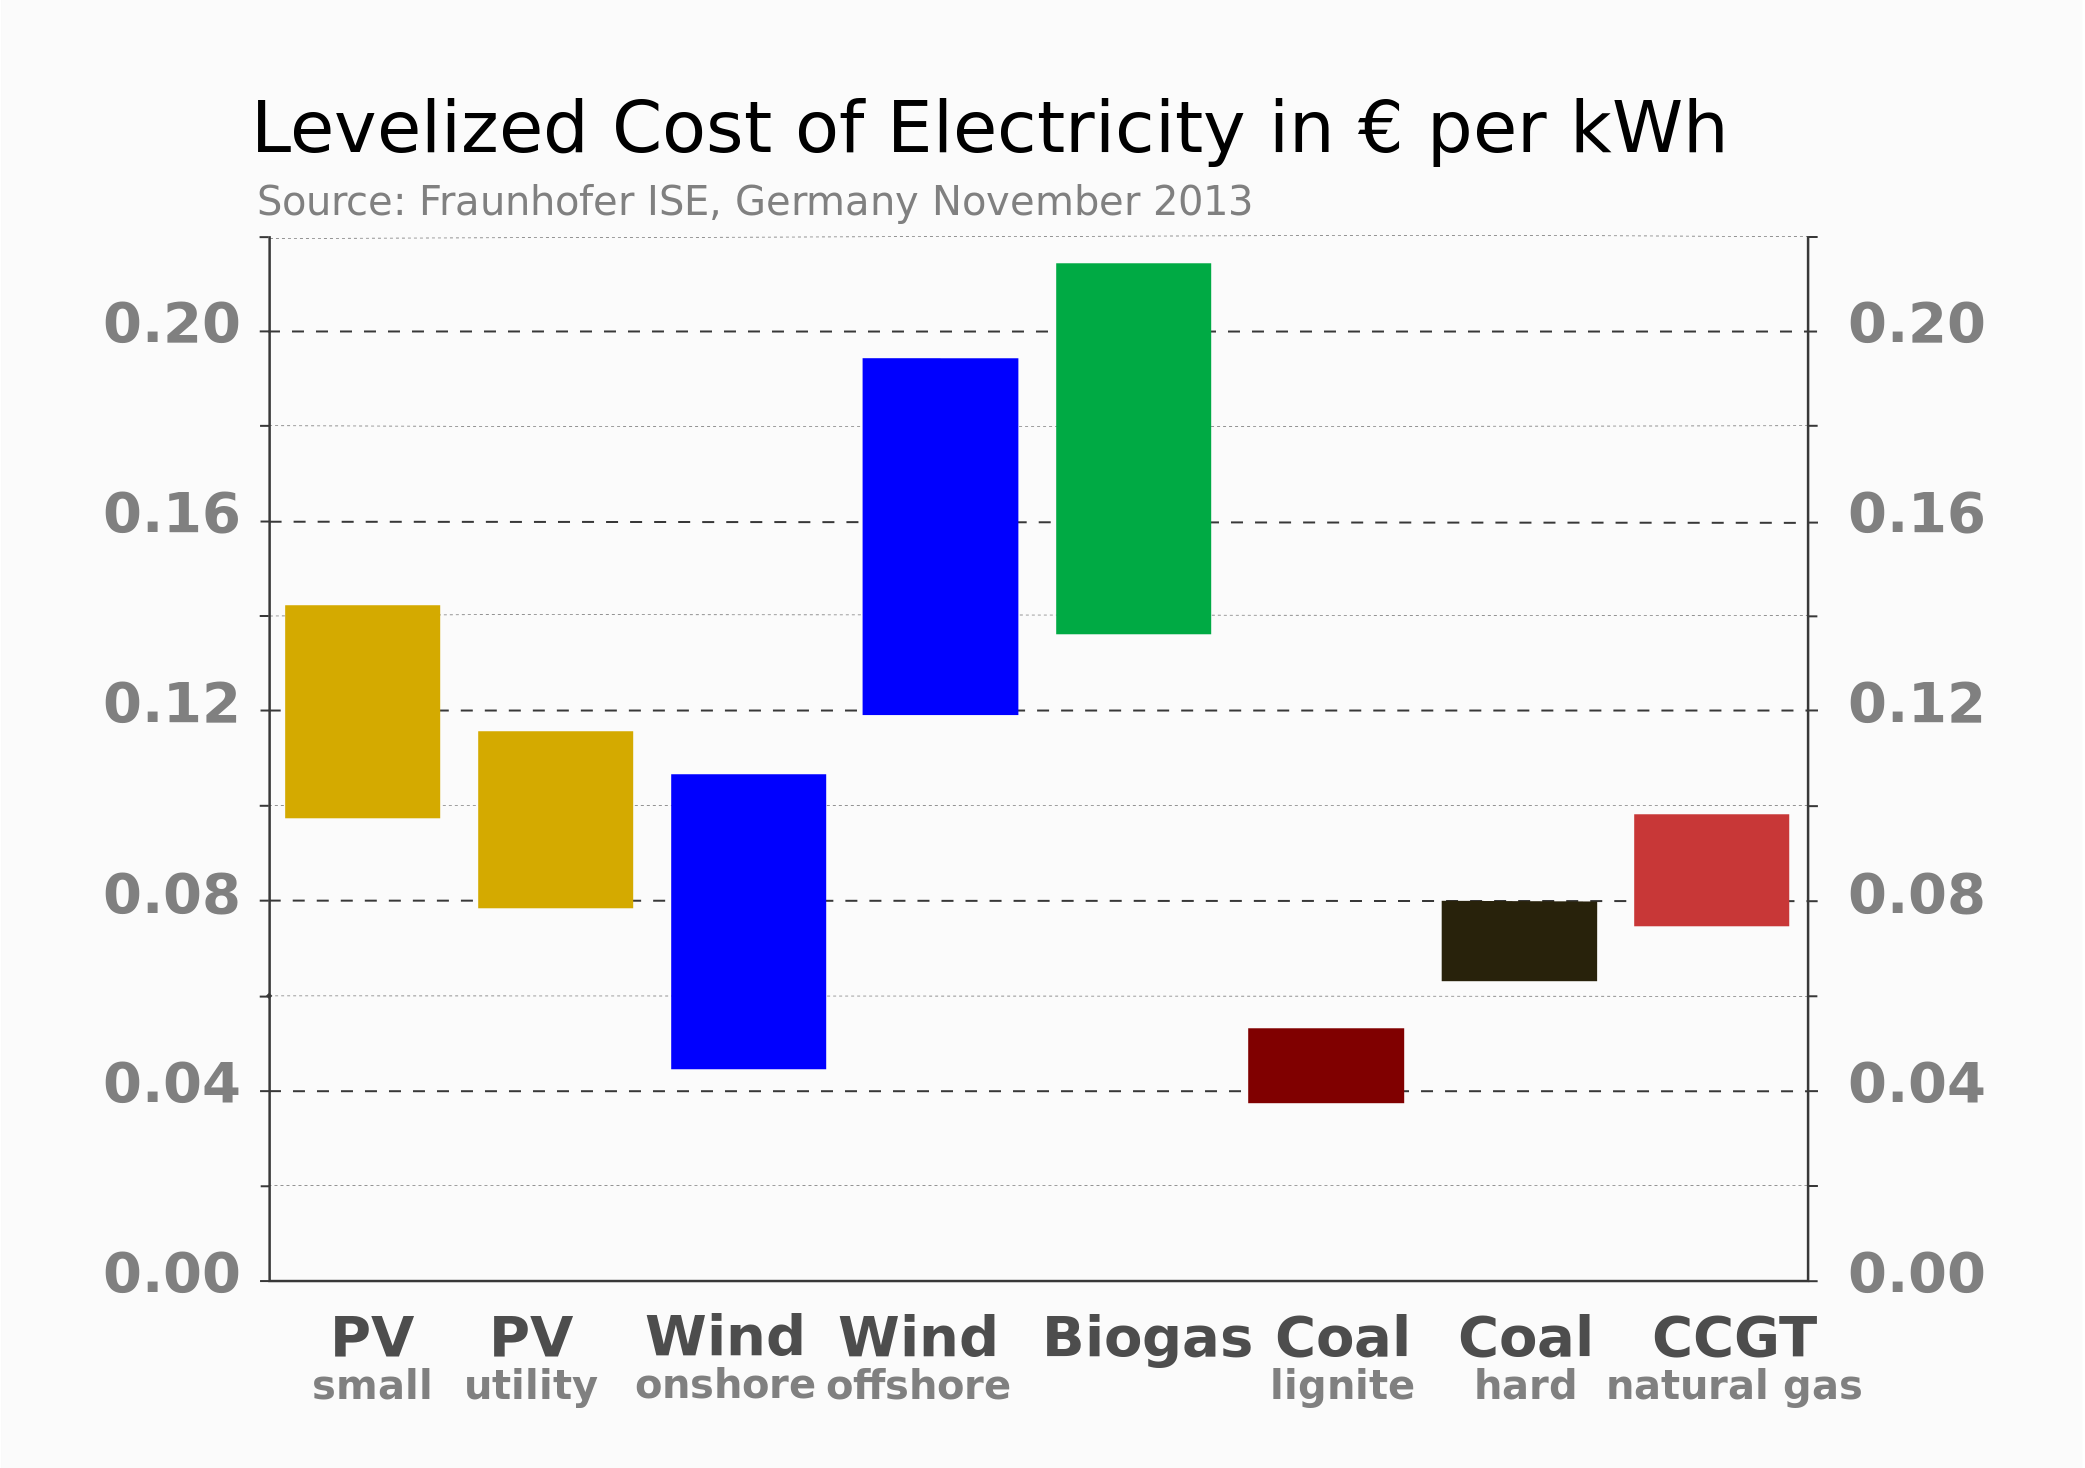
\includegraphics[width=0.8\textwidth]{figures/LCOE.png}
    \caption{Levelised cost of electricity (LCOE) of renewable energy technologies and conventional power plants at locations in Germany in 2013.  Specific investments are taken into account with a minimum and maximum value for each technology. Figure taken from reference \citenum{LCOE}.}
  \label{LCOE}
\end{figure}

%However if solar power, in combination with proper energy transport, storage and secondary conversion into heat and fuels, could be made to be economically feasible; it is a realistic candidate for replacing fossil fuels as a major supply of global energy. 

Levelised cost of energy, or electricity, (LCOE) is a common way to assess how cost competitive renewable energy sources are with their non-renewable counterparts. LCOE allows for the measurement of the performance of different power generating technologies, which may have unequal lifetimes and differing capacities. It is calculated by summing all costs incurred during the lifetime of the technology and dividing this value by the units of energy produced during the lifetime, with units of energy expressed as dollars per kilowatt hour (\$/kWhr) \cite{LCOE2}. This measure is also used as the key selling point for a number of commercial solar cell manufacturers such as First Solar Inc., who market their product as being able to generate electricity at an average of \$0.63 per Watt as stated in their 2013  Annual Report \cite{first_solar}. Using the LCOE, comparisons of grid competitiveness for renewable energy sources can be made \cite{LCOE2}. Figure \ref{LCOE} shows the LCOE of renewable energy technologies and conventional power plants at locations in Germany in 2013, enabling an assessment of the cost-competitiveness of PV power generation at this location, accounting for, for example, typical solar irradiation at the given locations \cite{LCOE}. As the figure shows, both small-scale and large-scale utility solar power are still not cost competitive with the cheapest non-renewable resources. In the next section, both commercial solar cell technologies that are currently available and emerging technologies are discussed to understand why solar power is currently not cost competitive, and how emerging technologies may be able to improve the status quo for global solar power generation.

%Germany is an example of a country making considerable efforts to increase the percentage of their energy supplied by solar power. 
%On the 9\textsuperscript{th} of June 2014 Germany even generated over 50\% of its electricity demand from solar for the first time \cite{Germany_guardian_news}. Although on average the country is not able to produce such a large portion from solar power, with solar-generated power providing approximately 7.5\% of net electricity consumption in 2015 \cite{Germany_PV}. 
%To facilitate the growth of the solar power capacity in Germany a number of schemes and financial incentives to encourage investment were introduced, such as feed-in tariffs (FiTs).

%\begin{figure}[h!]
%  \centering
%    \includegraphics[width=0.65\textwidth]{figures/global_energy.png}
%    \caption{Illustration of power available annually from various renewable energy resources, annual world energy consumption and total reserves of various non-renewable energy resources. Figure taken from reference \citenum{global_energy_fig}.}
%  \label{global_energy}
%\end{figure}

%\begin{figure}[h!]
%  \centering
%    \includegraphics[width=0.65\textwidth]{figures/BIPV.jpg}
%    \caption{A building integrated photovoltaics (BIPV) project fitted in the United States by BISEM-USA \cite{BIPV}.}
%  \label{BIPV}
%\end{figure}


\subsection{Current commercial solar cell technologies and limitations}\label{current_tech}
It was first observed in 1839 by Edmond Becquerel that sunlight could be used to generate electricity. Becquerel discovered that if  silver chloride was placed in an acidic solution, connected to platinum electrodes and exposed to sunlight, an electric current flowed. However the effect was small and poorly understood before Albert Einstein's discovery of the photoelectric effect and explanation of the phenomena by the quantum nature of light in 1904 \cite{PV_history1}. Even then, it was not until the development of semiconductor technology during the silicon revolution of the 1950's that solar cells were fabricated which were able to generate significant amounts of electricity. The first silicon solar cell was created in 1954 in the Bell Laboratories with cells achieving efficiencies of 6\%. 
Originally solar cells were developed for terrestrial energy generation, such as the 108 solar cells used to supply energy to the Vanguard satellite in 1958 \cite{PV_history1}. The first oil crisis in 1973 however highlighted the dependency of many economies on fossil fuels and the need to address the security of energy supply,  in particular for Japan and West Germany which had few of their own resources. As a consequence, solar cell research was no longer limited to only high-cost crystalline silicon devices for terrestrial applications, but also into creating cheaper, commercial, thin-film solar cell technologies using absorber materials such as amorphous silicon, cadmium telluride and copper indium diselenide  \cite{PV_history2}.

\begin{figure}[h!]
  \centering
    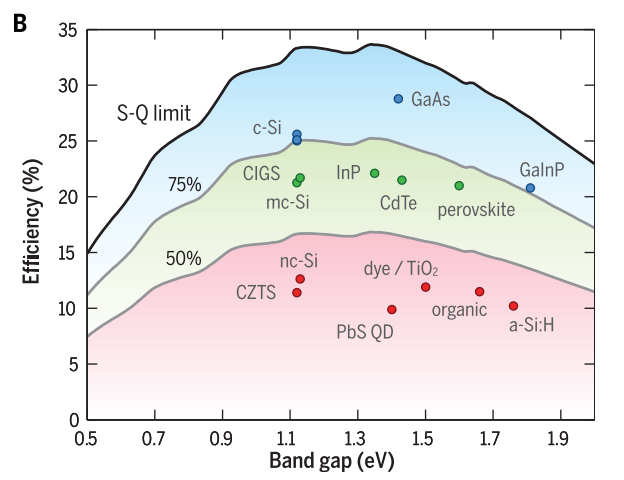
\includegraphics[width=0.75\textwidth]{figures/SQ_new.png}
    \caption{Theoretical Shockley-Queisser detailed-balance efficiency limit \cite{SQ_1961} as a function of band gap (highest black line) for AM1.5 solar spectrum. The record efficiencies for different materials are plotted for the corresponding band gaps, where materials below the lower two grey lines are achieving conversion efficiencies less than 75\% and 50\% of their theoretical efficiency limit respectively. Figure taken from reference \citenum{newPVrev}.}
  \label{SQ}
\end{figure}

Crystalline silicon is still the dominant solar cell technology with mono- and poly-crystalline silicon photovoltaic cells comprising up to 90\% of all the solar cells produced in 2008  \cite{Si_rev}. Silicon is the second most abundant element in the Earth's crust \cite{Si_abundance}. When considering this aspect alone, it seems to be a plausible material to use in large-scale solar power generation. Over 60 years of development have seen device efficiencies increase from 6\% to 25\% for the highest quality research devices and 15-18\% for the more common industrial cells \cite{Si_rev}. As can be seen from figure \ref{SQ}, the best performing silicon devices are now very close to achieving conversion efficiencies close to their theoretical limit, as predicted by Shockley-Quiesser \cite{SQ_1961}. More dramatic however is the fall in manufacturing costs which have halved since 2008 and are more than a hundred times lower than they were in 1977, as shown in figure \ref{Si_cost}. This development was largely aided by progress in semiconductor technology driven by the silicon chip industry, with the solar industry benefiting from advances in silicon manufacturing processes and even making use of waste silicon produced that was not of a high enough grade for silicon chips \cite{PV_history1}. Although the development of silicon-based technologies has clearly revolutionized the modern computer, the optical properties of silicon do not make it ideal for use as a solar absorber material in a photovoltaic device and despite the dramatic reduction in manufacturing costs, the technology is still not able to be cost-competitive with fossil-fuel power generation, as was shown in figure \ref{LCOE}.

\begin{figure}[h!]
  \centering
    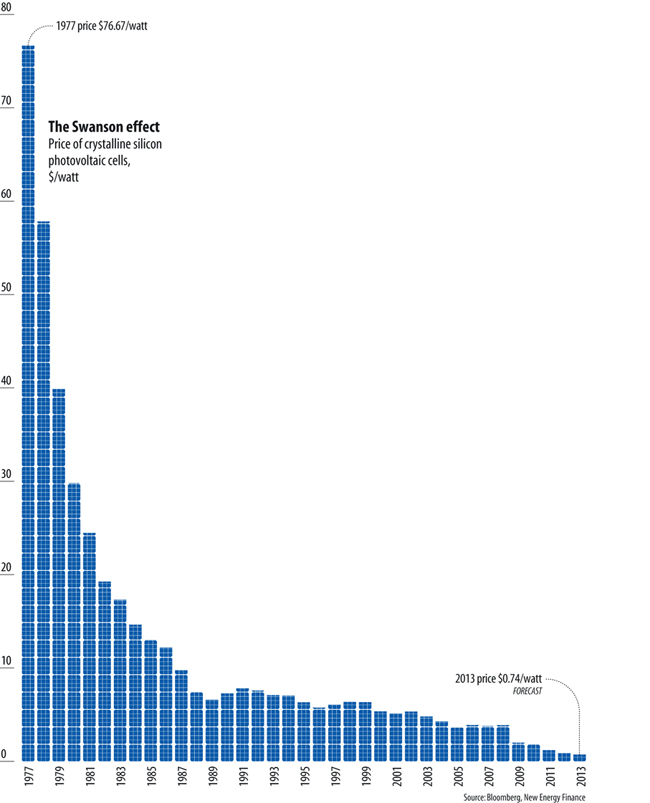
\includegraphics[width=0.8\textwidth]{figures/Si_cost.jpg}
    \caption{Average cost of solar panels composed of a crystalline silicon absorber layer. Figure taken from reference \citenum{PV_chart}.}
  \label{Si_cost}
\end{figure}

The primary issue with silicon is that its band gap of 1.1 eV is indirect. The importance of the electronic band gap in relation to PV performance will be discussed further in section \ref{PV_properties}. For now, it is just noted that the key consequence of the indirect nature of the band gap of silicon is that it is not a very strong absorber of sunlight (compared to for instance newer, thin-film technologies which are discussed next), resulting in a low optical absorption coefficient  compared to these newer technologies. To absorb the same amount of sunlight with a silicon solar cell requires a thicker layer of the material than in thin-film technologies. Photovoltaic devices are very sensitive to defects and impurities. This point is discussed further in section \ref{defects_impact}, but the consequence for a thick layer of silicon is that very high quality, non-defective material is necessary to enable charge carrier collection before electron-hole recombination occurs, which results in high manufacturing costs. The devices are made from flat sheets of crystalline or multi-crystalline silicon called wafers that consist of very high quality silicon (99.999999\% pure) 
\cite{sus_book_5}.
The production processes of silicon wafers have been thoroughly optimised, but are still very energy-intensive, time-consuming and complex \cite{emerging_pv}.
%and this is reflected by the position of this type of technology on the plot of efficiency versus cost shown in figure \ref{PV_generations}. 
Despite decades of development, commercial silicon solar panels are still too expensive to compete with fossil-fuel based power sources \cite{FE_PV_rev1_5}. 

%\begin{figure}[h!]
%  \centering
%    \includegraphics[width=0.75\textwidth]{figures/PV_generations.png}
%    \caption{Efficiency and cost projections for first-, second- and third-generation photovoltaic technologies, which are comprised of silicon wafer, thin-film and advanced thin-film technology respectively. Figure  taken from reference \citenum{sus_book}.}
%  \label{PV_generations}
%\end{figure}

The `holy grail' of research into new materials for photovoltaic devices would be to find materials that are strong absorbers of sunlight, could be produced cost-effectively and composed of materials that are abundant enough for large-scale fabrication of the devices. 
%Such a drive has resulted in the development of what are considered three generations of solar energy technology. These are shown in figure \ref{PV_generations}, where highly efficient crystalline silicon devices with high associated manufacturing costs are considered the first generation of solar cell technology.
Thin-film solar cell devices make use of materials that are much more optically thick than silicon (i.e. stronger absorbers of sunlight with direct optical band gaps and higher optical absorption coefficients), which require less material to absorb the same amount of sunlight. %Figure \ref{thin_films} shows a comparison between the thickness of the aborber layer in some commercial second-generation PV devices to that of first-generation silicon wafers. 
The consequence of the reduction in the thickness of the absorber layer is that it is then less important for the material to be of as high-quality as in crystalline silicon devices, which enables the use of low-cost and low-energy fabrication methods \cite{emerging_pv}. Many thin-film technologies are also light-weight and flexible, allowing for more options for innovative deployment of the modules, such as building integrated photovoltaics (BIPV) and portable devices.

%Typically the efficiencies of second-generation solar cells are less than that of the best performing first-generation devices. 
Examples of commercial thin-film technologies include CIGS (Cu(In,Ga)(S,Se)$_2$) and CdTe. 
In the case of thin-film CuInSe$_2$ devices, it has even been found that the `lower quality' poly-crystalline material has a higher performance than its single crystal counterpart \cite{CIS1_3, CIS1_4}. Theoretical studies of the electronic properties of the grain boundaries in CuInSe$_2$ have provided an explanation for this unusual observation based on beneficial band offsets at the grain boundaries \cite{CIS1, CIS2}. This effect is a special case for this material, but it embodies the general ideology of thin-film technology well - namely to produce materials able to convert sunlight into electricity as efficiently as possible, with the simplest synthesis techniques possible.
Other innovations in PV technology include the use of multiple energy threshold devices to overcome the Shockley-Quiesser limit \cite{SQ_1961} for a single band gap solar cell, such as in tandem solar cells where semiconductor p-n junctions of increasing band gap are placed on top of each other in order to capture more of the solar spectrum. Typically these more complicated device architectures result in higher fabrication costs. Research efforts are therefore largely focused on reducing the fabrication cost of multi-junction devices \cite{3rd_gen}.

%\begin{figure}[h!]
%  \centering
%    \includegraphics[width=0.9\textwidth]{figures/thin_films2.png}
%    \caption{Typical structures of a commercial wafer-based PV device (first left) and commercial thin-film photovoltaic devices, as well as a CZTS thin-film device (right). The absorber layers are labelled in white and thickness is shown to scale. Figure adapted from reference \citenum{pathways}.}
%  \label{thin_films}
%\end{figure}

Current mainstream solar cell technologies, such as Si wafers and thin-film CdTe and CIGS solar cells, are unlikely to be able to provide solar electricity at the terawatt scale due to the scarcity of Te and In and the relatively long energy payback time for crystalline Si due to the cost and energy intensive fabrication of Si wafers \cite{CZTS_vs_MAPI}. 
Models have quantified such statements with a predicted In-constrained growth potential of power generation from CIGS PV technology of ~20 GW per year in 2020 due to competing applications of In, such as in liquid crystal displays \cite{culprit_5_3}.
To significantly increase the contribution of solar power to the global power supply, it is therefore necessary to develop more economically viable earth-abundant materials for sustainable PV electricity generation. Furthermore, there must be considerable technological breakthroughs that would enable low-cost manufacturing of highly efficient devices with enough of a cost benefit to outweigh the initial cost outlay in optimising the manufacturing process of the whole device as has been done for silicon over the past 60 years. For this purpose, there is a drive for solar absorber materials with more optimal properties, such as a direct and sunlight matched band gap (as in thin-film technologies such as CdTe and CIGS), but also for materials that are composed of only earth-abundant components.\\

** Add data on elemental abundance here and comment on in text **

\subsection{Examples of emerging metal sulfide solar absorbers}

The magnitude of the optical band gap is the most fundamental, necessary property of a semiconductor in order to have the potential to produce a high-efficiency solar cell device. Other important material properties for the absorber material in a PV device are discussed in section \ref{PV_properties}, but for now it is just noted that to maximise the energy harvesting potential of the PV device, a band gap for the absorber that is direct in nature and closely matched to the major component of the solar spectrum is desirable, this corresponds to a range of approximately 1.0 to 1.7 eV \cite{PV_E_range}. The optical band gap is the most fundamental and obvious screening criteria to use when selecting new candidate absorber materials for photovoltaic devices. The band structure of semiconductors will be discussed further in section \ref{BandTheorySection}, but for now it will just be noted that metal tellurides, selenides and sulfides typically have band gaps within the optimal energy range for PV applications due to the chalcognide p-orbital (which is usually the dominant component of the valence band maximum) being higher in energy than, for instance, the oxygen p-orbitals in metal oxides, which typically have band gaps that are too wide for PV applications. Of metal tellurides, selenides and sulfides, sulfur stands out in the interests of abundance and minimising toxicity.

SnS is an example of a non-toxic and earth-abundant metal sulfide that has received research interest for solar cell applications. SnS has a direct band gap within the optimal range for sunlight absorption of between 1.30 eV \cite{Lee_thesis_59} and 1.43 eV \cite{Lee_thesis_60}. However, record power conversion efficiencies (PCE) of PV devices are at around just 4\% \cite{SnS_record}. The low-performance of SnS devices has been attributed to several factors including the defect physics \cite{Lee_SnS_defects}, non-optimal band alignment in devices \cite{Lee_SnS_band} and phase impurity \cite{Lee_SnS_phases} of the material.
Kesterite-structured {\CZTS} (CZTS) has also received a large amount of research interest for PV applications, also due to the highly desirable earth-abundance and non-toxicity of its constituent elements, along with promising optical properties. The band gap of CZTS has been predicted \cite{CZTS_bandgap_theory} and measured \cite{CZTS_bandgap_exp} to be direct with a magnitude of 1.5 eV. 
The record device efficiencies are more than double that of SnS-based solar cells. However, CZTS solar cells still fall far short of their theoretical maximum PCE of 28\% predicted from the Shockley-Quiesser limit based on the optical band gap. The current confirmed record device efficiency of a sulfide-selenide alloy is 12.6\% \cite{Mitzi2017_rev_21}, while that of the pure sulfide material lags even further behind at behind at 9.1\% \cite{CZTS_record}. A large component of this work seeks to investigate possible origins of the performance deficit of CZTS solar cells. The other major component of this work looks to identify photoactive ferroelectric (or `photoferroic') materials so that alternative routes to high-efficiency solar cells may be explored by exploiting novel PV phenomena observed in ferroelectric materials. This is discussed in more detail in section \ref{ferroPVsection}. 


\section{The role of computational modeling in material design and optimisation}
The discovery of new functional materials by experimental methods is largely hindered by high costs and the optimisation of time-consuming synthesis procedures \cite{high_tp}.
However, with the rapid increase in computational processing power and the availability of large-scale supercomputers, we are entering a very exciting era in computational materials design \cite{WMD_material_design_review}. Furthermore, electronic structure theory has advanced to a level where it is possible to obtain good quantitative agreement with experiment without using adjustable parameters fit to experiment, i.e. from first principles. The only inputs into these calculations are electronic mass, electronic charge, atomic numbers and masses of the constituent atoms in the material. From this, it is possible to obtain to fairly high accuracy the structure, lattice constants, charge densities and various electronic, magnetic, optical and transport properties \cite{elec_structure_theory}. Therefore theory and simulation of materials has reached a point of possessing some predictive power for material properties relevant for various applications, completely independent of experimental measurement.

There are two main contributions that computational simulations could make towards the technological breakthroughs needed for economically-viable, large-scale solar energy generation. Firstly, by predicting relevant properties of materials that are not currently utilised in solar cells and screening for certain desirable properties, material simulations are able to aid in the discovery of new materials that may be capable of out-performing current solar cell technologies. Such an approach allows for a less time-consuming screening of potential new materials for a given application before attempting to prepare just the most promising candidates in the laboratory. Experimental validation of predicted properties, however, is always an important follow up to account for additional features of the physical system not initially accounted for in the model. In the case of candidate solar absorbers, for example, the optical properties are often initially predicted for the perfect bulk crystal. In reality materials contain various types of defects. Methods exist to model different forms of defects in a crystalline system, some of which are discussed later in this work. However, this typically quite complex and idiosyncratic feature of the system is often not considered initially, largely due to the vast range of possible defect features in a material. The defect physics of a material is a prime example of an area in which knowledge and understanding is developed symbiotically between works from experiment and theory. Secondly, material simulations are able to provide valuable, atomistic insight on scales that cannot be probed experimentally to improve fundamental understanding of known photovoltaic materials, which may enable improvements in existing solar cell technologies. Defect physics is again a prime example of this, where theory can probe on the atomic scale to aid in the interpretation of experimental data obtained from a variety of different measurements.

In this work, materials modeling techniques are developed and applied to make both types of contribution to the field. A model is developed to improve current atomic-scale understanding of the candidate earth-abundant, non-toxic solar absorber material {\CZTS} (CZTS) and to provide a tool for assessing possible origins of the under-performance of this particular solar cell technology. This is the subject of \autoref{chap:CZTS}. Materials modeling is also used to predict the relevant properties of candidate photoferroic absorbers that are not currently utilised in solar cell technologies to identify those that are most likely to be worthy of further study. In \autoref{chap:screening}, the screening criteria and methodologies used in this study for identifying candidate photoferroic absorbers are discussed and some relevant calculated material properties for the candidates are presented. In \autoref{chap:insights}, the use of material simulations and theoretical insights to assess the likely performance of a material in a solar cell device is discussed further. In particular, knowledge gained from previous studies on more mature PV technologies is drawn upon when examining the potential of the candidate photoferroic materials for solar cell applications.

\section{Format of thesis}
Statement about incorporating papers into thesis (and which sections correspond to papers)? Need a statement about personal contributions? - especially Eris adapted by Jarv from original starrynight code, materials screening with Lee and defects benchmark study with various collaborators and development with FHI-aims developers

\chapter{Theoretical background} 

\section{Models of perfect, periodic solids}\label{crystal_models}
%Refer to: pg 28 29 35 \cite{thin_film_Boer}\\
To relate the properties observed for a material to its underlying atomic and electronic structure, and also to predict properties that have not yet been measured, it is necessary to have a suitable model for the material. Theoretical models of crystalline solids are based around the existence of translational symmetry in a crystal lattice such that the lattice can be constructed by periodically repeating a unit cell of atoms. The Bravais lattice specifies the periodic array in which the repeated units of the crystal are arranged. A crystal lattice can therefore be described by its underlying Bravais lattice and the arrangement of atoms, ions or molecules within a particular unit cell, i.e. the basis \cite{AshcroftMermin2}. This principle is also used in electronic calculations of solid state systems through the implementation of periodic boundary conditions to simulate an infinite, bulk system using only a finite unit cell. Methodologies used in electronic structure calculations will be discussed further in section \ref{elec_struc}.
 
Another important concept in the theoretical modeling of periodic structures is reciprocal space and the reciprocal lattice. 
Converting to reciprocal space enables the description of periodic features with a longer-range periodicity than the unit cell in real space, such as the motion of electrons in a crystal and phonons.
%In the same way that any quantity that varies with time can be described as a sum of Fourier components in the frequency domain; 
The spatial properties of a crystal can be described as a sum of components in Fourier space, otherwise known as reciprocal space or \textit{k}-space. The reciprocal lattice of a perfect single crystal is an infinite periodic 3D array of points whose spacings are inversely proportional to the distances between the planes in the lattice in real space. Vectors in real space have dimensions of length, whereas vectors in reciprocal space have dimensions of length$^{-1}$. This can therefore be compared directly to the wavevector $ \left(k  = \frac{2\pi}{\lambda} \right)$ of an excitation such as a phonon or a moving electron and multiplication of each coordinate of the reciprocal lattice by $\hbar$ converts reciprocal space into momentum space as for a quantised wave $\mathbf{p} = \hbar \mathbf{k}$ \cite{Blakemore1}. 

\begin{figure}[h!]
  \centering
    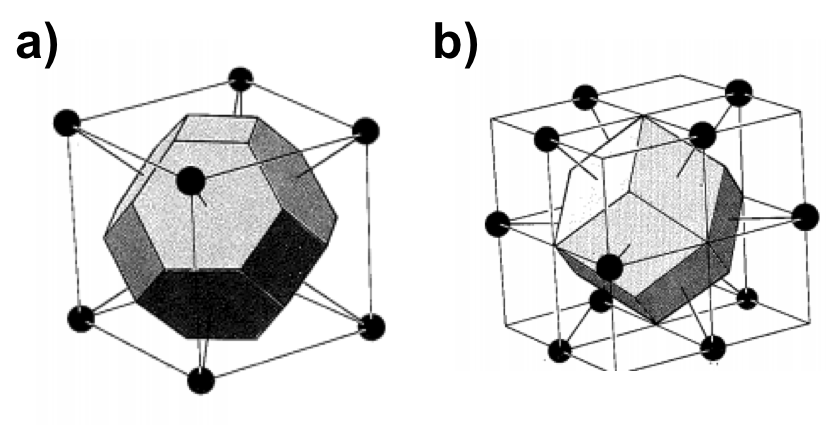
\includegraphics[width=0.5\textwidth]{figures/Wigner-Seitz.png}
    \caption{The Wigner-Seitz cell for the body-centred cubic Bravais lattice where there is a lattice point at its centre and on each vertex (a) and the face-centred cubic Bravais lattice (b). 
    %The hexagonal faces bisect the lines joining the central point to the points on the vertices. The square faces bisect the lines joining the central point to the central points in each of the six neighbouring cubic cells. 
    Figure taken from reference \citenum{AshcroftMermin2}.}
  \label{Wigner-Seitz}
\end{figure}

The Wigner-Seitz primitive cell is the most common choice of primitive cell with the full symmetry of the Bravais lattice. It represents the region of space around a lattice point  that is closer to that point than to any other lattice point. For example, figure \ref{Wigner-Seitz}a shows the truncated octahedron that is the Wigner-Seitz cell for a body-centred cubic (bcc) lattice \cite{AshcroftMermin2}.
The first Brillouin zone is the Wigner-Seitz primitive cell of the reciprocal lattice. The reciprocal of the bcc lattice is face-centred cubic (fcc), therefore the first Brillouin zone of the bcc lattice is the fcc Wigner-Seitz primitive cell as shown in figure \ref{Wigner-Seitz}b \cite{AshcroftMermin3}. As the full symmetry of the reciprocal lattice is contained within the first Brillouin zone, it is only necessary to sample \textit{k}-points within this single unit cell of the reciprocal lattice when calculating the electronic ground state of a periodic structure.



\section{Electronic band structure of semiconductors}\label{BandTheorySection}
%Refer to: pg 18 \cite{fund_semi}, pg 105 112 128 131 137 \cite{thin_film_Boer}, pg 111 + 119 \cite{phys_semicond}\\
%** Highlight link to PV and indication of PV performance from band structure + check against Nelson CH3\\
%The band theory of solids provides a means to explain the difference in the electrical conductivity of conductors, semiconductors and insulators. 
Electrons bound to an atom in atomic orbitals have a number of possible discrete energy levels. When a pair of atoms are brought together to form a molecule, the atomic orbitals combine to form pairs of molecular orbitals arranged with energy levels slightly higher and slightly lower in energy than the original energy levels. When a large number of atoms are brought together to form a solid the 
%it becomes impossible to assign individual electrons to individual atoms. Instead, the electrons are considered to be shared amongst the atomic nuclei. A consequence of this sharing would be a large number of electrons occupying the same energy state, which violates the Pauli Exclusion Principle. The 
original discrete energy levels are broadened into new energy levels that are so closely spaced that they are considered to be a quasi-continuous band of allowed energies. This is illustrated in Fig. \ref{band_Elevels}. The energy distribution of the bands depends upon the electronic properties of the constituent atoms of the crystal and the strength of the bonds between them. Bands are occupied if the original molecular orbitals were occupied. The highest occupied band (containing the valence electrons) is the valence band (VB). The lowest unoccupied band is the conduction band (CB). If the VB is only partially filled or if it overlaps in energy with the CB, then the solid is a metal. The availability of empty states at energies close to that of the occupied states facilitates easy scattering of valence electrons into neighbouring states, thereby allowing for the transport of heat and charge. Hence metals conduct both heat and electric current. In a semiconductor or insulator, the VB is completely full and separated from the next unoccupied CB by an energy gap called the optical band gap, E$_g$ \cite{Nelson3}. In the simplest model, the CB is separated from the VB by a constant band gap. This is called the flat band model and is often shown in schematics of junctions for PV device architectures, which will be discussed in section \ref{junctions}. In real structures, the band architecture is more complicated than this simple model, like the band structures shown later in figure \ref{Si_and_GaAs} \cite{Tilley}.

\begin{figure}[h!]
  \centering
    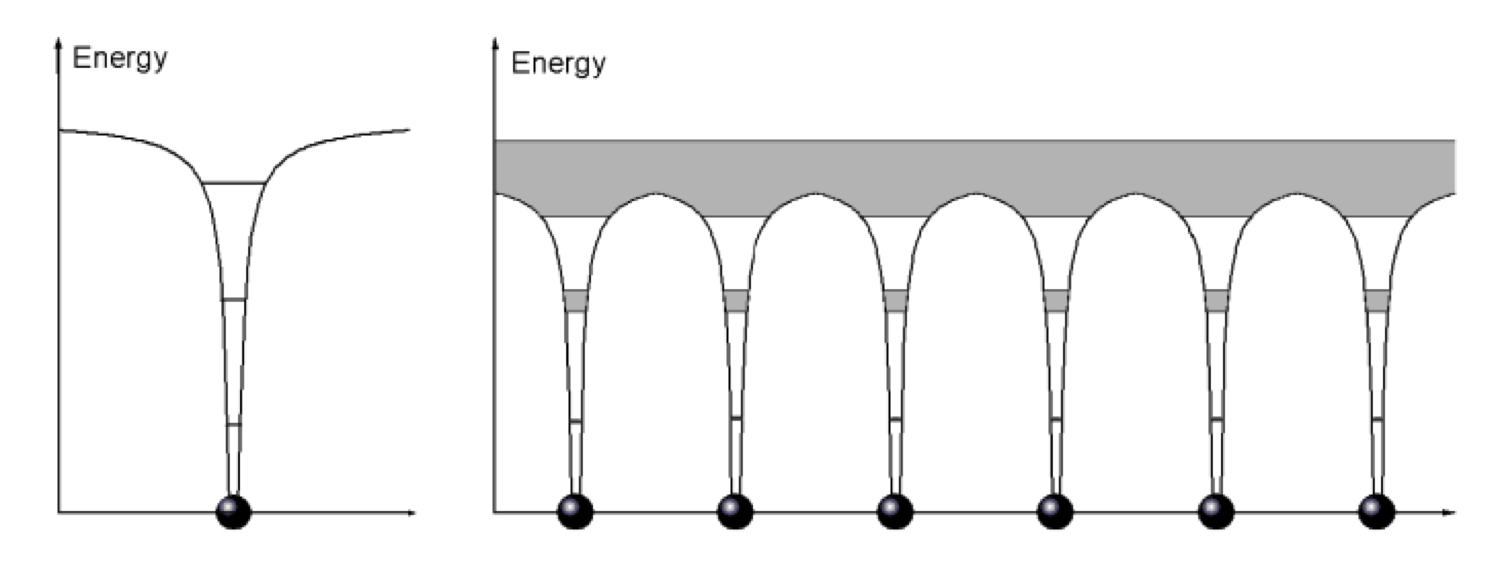
\includegraphics[width=0.7\textwidth]{figures/band_Elevels.png}
    \caption{Electron energy levels of a single atom (left) and the formation of a quasi-continuous band of allowed energies in a solid crystal when many atoms are brought close together (right). Figure taken from \citenum{mat_prop1}.}
  \label{band_Elevels}
\end{figure}

To understand the behaviour of electrons in solids, the electron is considered as a wave propagating in a periodic structure \cite{small_semiconductor1}. The Schr{\"o}dinger equation (SE) must be solved to determine the energy of electrons in a solid. 
The energy of a single electron in a perfect crystal is described by the one-electron Schr{\"o}dinger equation, shown in equation \ref{single_SE}. The first term in equation \ref{single_SE} is the kinetic energy of the electron, V(\textbf{r}) is the effective periodic potential energy experienced by the electron in the crystal, $\psi$ is the electron wavefunction and $\epsilon$ is the eigenenergy of the electron.
\begin{equation} \label{single_SE}
\left[ \left(-\frac{\hbar^2}{2m}\right)\nabla^2 + V(\mathbf{r})\right]\psi = \epsilon \psi 
\end{equation}
For a solid the infinite array of atomic potentials making up the crystal must be accounted for, as opposed to just the few associated with a molecule. For this purpose, the periodicity of crystalline solids outlined in section \ref{crystal_models} is exploited to determine the probability distribution of electrons in an infinite solid \cite{Nelson3}. 
The spatial dependence of the potential experienced by an outer electron in a crystal for multi-electron systems was considered by Felix Bloch. Bloch determined that the total potential is the sum of two parts. Firstly, the electrostatic potential due to the array of atomic cores. For a perfect lattice this should have the translational periodicity of the lattice. Secondly, the potential due to all other electrons. Bloch assumed that the charge density would have the same long-term average value in every unit cell of the crystal and therefore would be periodic \cite{fund_semi}.
The periodicity of the crystal lattice means that the probability distribution of the electrons must also be periodic, with no preference for an electron to occupy a particular site within one unit cell than any others. Furthermore, as the lattice is infinite, electrons in a periodic solid should form delocalised states which extend throughout the crystal in a similar manner to an electron in free space.
Bloch's theorem states that the wavefunction which satisfies equation \ref{single_SE}, subject to a periodic potential, should be of the form shown in Eq. \ref{bloch}. This Bloch wavefunction is a product of a function $U_{i\mathbf{k}}(\mathbf{r})$, which possesses the periodicity of the lattice, and a plane wave part, where \textbf{k} is the wavevector of an electron propagating in the crystal bands i \cite{Nelson3}.
\begin{equation} \label{bloch}
\phi_k(\mathbf{r}) = U_{i\mathbf{k}}(\mathbf{r}) e^{i\mathbf{k \cdot r}} 
\end{equation}
\begin{equation} \label{bloch_sum}
\psi_k(\mathbf{r}) = \sum_k A_k \phi_k(\mathbf{r}) = \sum_k A_{i\mathbf{k}}U_{i\mathbf{k}}(\mathbf{r}) e^{i\mathbf{k \cdot r}} 
\end{equation}
Due to the translational symmetry of a crystal lattice, an eigenfunction of the one-electron Schr{\"o}dinger equation can be expressed as a sum of Bloch functions such as that shown in equation \ref{bloch}, to give Eq. \ref{bloch_sum}. The one-electron wavefunctions can be indexed by constants \textbf{k} and i \cite{fund_semi}. 
$U_{i\mathbf{k}}(\mathbf{r})$ and electron eigenenergies, $\epsilon(\mathbf{k})$, from Eq. \ref{single_SE} are found by solving the SE for each band i and for each \textbf{k} \cite{Nelson3}.
A plot of $\epsilon(\textbf{k})$ versus \textbf{k} is known as the energy dispersion relation or electronic band structure of the crystal \cite{fund_semi}.
\begin{figure}[h!]
  \centering
    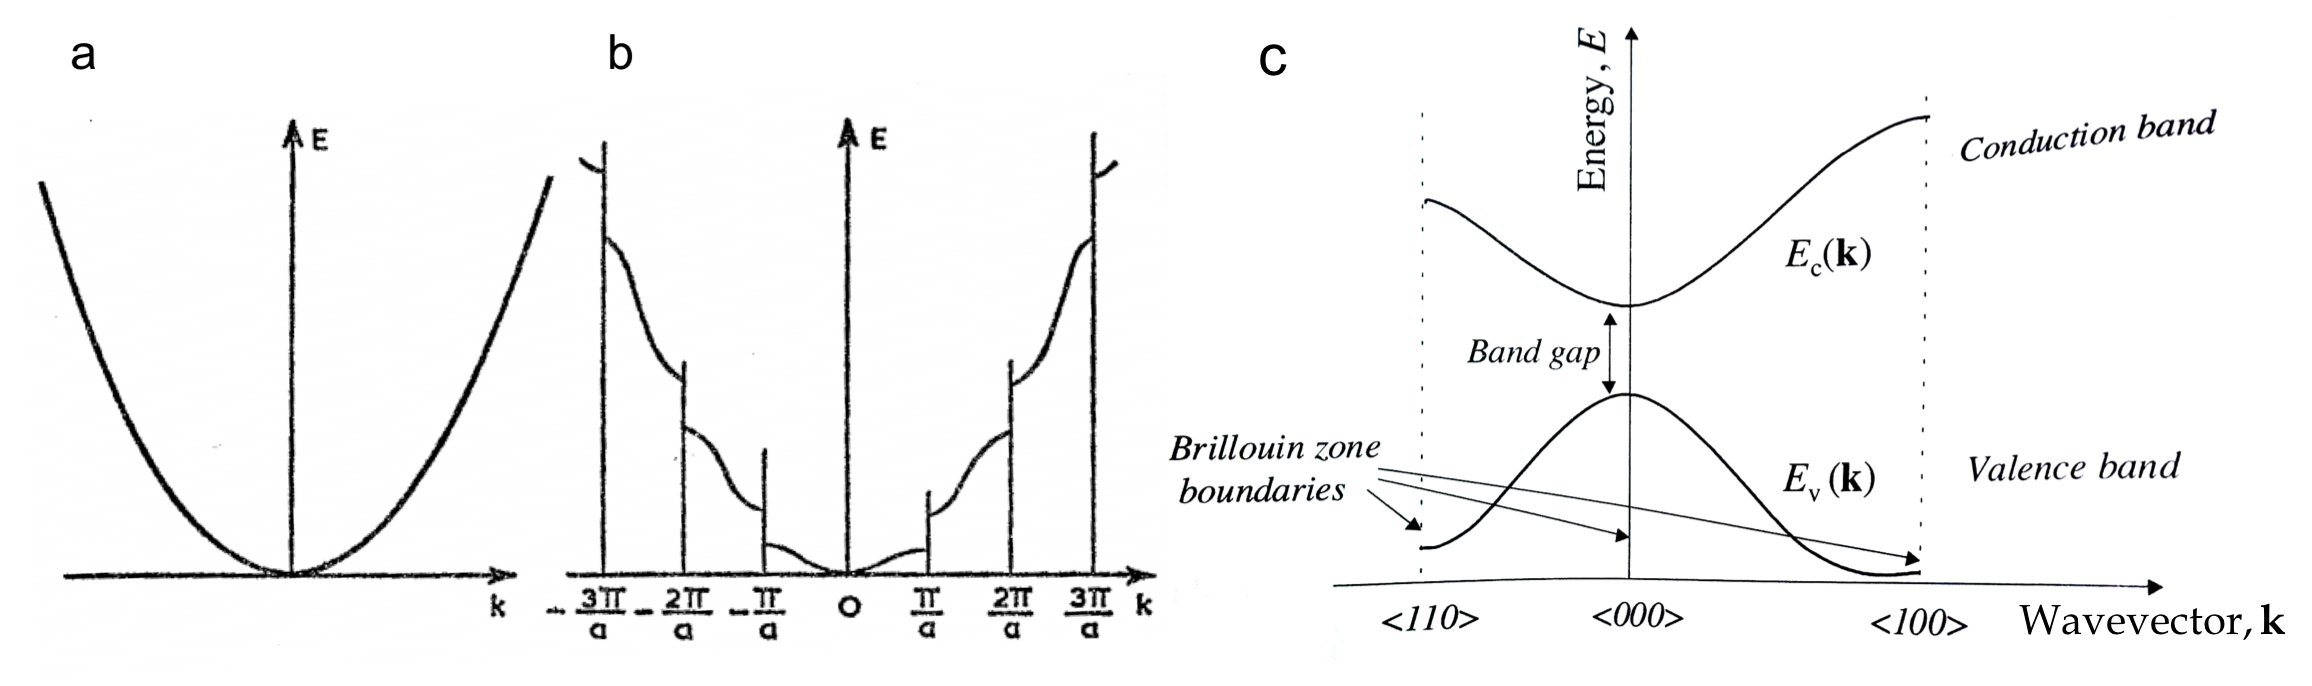
\includegraphics[width=0.95\textwidth]{figures/bs1_2.png}
    \caption{Energy-wave vector diagrams: (a) the free electron parabola, (b) modification due to a periodic crystal lattice. Figures a and b taken from Ref. \citenum{small_semiconductor1}, figure c taken from Ref. \citenum{Nelson3}.}
  \label{bs1}
\end{figure}

The impact of a medium with a discrete structure, such as a crystal lattice, on the energy dispersion relation of a free electron can be seen by comparing Fig \ref{bs1}a to Fig. \ref{bs1}b.
The band structure, E(\textbf{k}), of a material is usually plotted against $|\textbf{k}|$ just for the most important directions in the crystal, such as that shown in Fig. \ref{bs1}c. A periodic medium does not suppress the propagation of waves, as would be expected in disordered or amorphous structures, but introduces limiting frequencies and wavelengths for the propagation. 
The parabola of the free electron is modified in a periodic crystal by the introduction of discontinuities at values of $|\textbf{k}|$ corresponding to multiples of $\frac{\pi}{a}$, as shown by Fig. \ref{bs1}b \cite{small_semiconductor2}. The point $|\textbf{k}| = \frac{\pi}{a}$ is the Brillouin zone boundary. At these points the electron wavefunction is a standing wave and the gradient of E(\textbf{k}) disappears \cite{Nelson3}.
The lower limit of the wavelength is set by the lattice spacing, giving an upper limit of the wave vector, $|\textbf{k}|$, of $\frac{\pi}{a}$, where a is the spacing of the planes of atoms in the direction E(\textbf{k}) has been plotted.  The appearance of such energy gaps implies that electrons in a periodic crystal may only have kinetic energies corresponding to certain bands, whilst being free to propagate in the lattice \cite{small_semiconductor2}. 
Due to the periodicity of the crystal lattice, $|\textbf{k}|$  that differ by multiples of $\frac{2\pi}{a}$ cannot be distinguished and E(\textbf{k}) repeats for $|\textbf{k}| > \frac{\pi}{a}$. For most crystals for $|\textbf{k}| < 0$, E(\textbf{k}) is identical to E(\textbf{-k}) since states with positive and negative $|\textbf{k}|$ are degenerate. Therefore all information for the energy dispersion relation, E(\textbf{k}) vs. $|\textbf{k}|$, of the material is contained in the range $0 < |\textbf{k}| < \frac{\pi}{a}$ and so only this region needs to be plotted, as in Fig \ref{bs1}c \cite{Nelson3}. 

A useful concept used to simplify the dynamics of an electron in a crystal lattice in the band theory of solids is that of effective mass. The effective mass is a convenient parameter determined by the curvature of of the maxima and minima of the VB and CB respectively to account for the influence of a periodic lattice on a free carrier, enabling an electron in a periodic crystal to be treated as though it were a free particle but with a different mass in calculations of charge transport \cite{small_semiconductor2}.
%$U_{i\textbf{k}}(\mathbf{r})$ depends weakly on \textbf{k}, but this dependence is neglected in the effective mass approximation \cite{Nelson3}.
The influence of the effective mass of charge carriers in a solar absorber material on the efficiency of a PV device composed of that material will be discussed in section \ref{PV_properties}.

%The concept of the energy band model of a solid emerges from considering the behaviour of electrons in a periodic crystal lattice, but cannot be understood in terms of classical physics alone. Instead, the electron must be considered in terms of wave-mechanical terms as a wave propagating in a periodic structure with diffraction and interference effects  \cite{small_semiconductor1}.
%In the band theory of solids, the energy of a single electron in a perfect crystal is described by the one-electron Schr{\"o}dinger equation, shown in equation \ref{single_SE}. The first term in equation \ref{single_SE} is the kinetic energy of the electron, V(\textbf{r}) is the effective non-zero periodic potential energy experienced by the electron in the crystal, $\psi$ is the electron wavefunction and  $\epsilon$ is the eigenenergy of the electron. In band theory, it is assumed that for any electron, everything else in the crystal can be represented by the effective potential energy, V(\textbf{r}) \cite{Blakemore2}.
%\begin{equation} \label{single_SE}
%\left[ \left(-\frac{\hbar^2}{2m}\right)\nabla^2 + V(\mathbf{r})\right]\psi = \epsilon \psi 
%\end{equation}
%The spatial dependence of the potential experienced by an outer electron in a crystal for multi-electron systems was considered by Felix Bloch. Bloch determined that the total potential is the sum of two parts. Firstly, the electrostatic potential due to the array of atomic cores. For a perfect lattice this should have the translational periodicity of the lattice. Secondly, the potential due to all other electrons. Bloch assumed that the charge density would have the same long-term average value in every unit cell of the crystal and therefore would be periodic. Bloch's theorem states that the wavefunction which satisfies equation \ref{single_SE} subject to a periodic potential should be of the form shown in equation \ref{bloch}, where $U_k(\mathbf{r})$ is some function 
%(depending on the value of the wavevector, \textbf{k}) that also has the complete periodicity of the lattice and \textbf{k} is confined to the first Brillouin zone \cite{Blakemore2}.
%\begin{equation} \label{bloch}
%\phi_k(\mathbf{r}) = U_k(\mathbf{r}) e^{i\mathbf{k \cdot r}} 
%\end{equation}
%\begin{equation} \label{bloch_sum}
%\psi_k(\mathbf{r}) = \sum_k A_k \phi_k(\mathbf{r}) = \sum_k A_kU_k(\mathbf{r}) e^{i\mathbf{k \cdot r}} 
%\end{equation}
%Due to the translational symmetry of a crystal lattice, an eigenfunction of the one-electron Schr{\"o}dinger equation can be expressed as a sum of Bloch functions such as that shown in equation \ref{bloch}, to give equation \ref{bloch_sum}. The one-electron wavefunctions therefore can be indexed by constants \textbf{k}, which are the wave vectors of the plane waves forming the `backbone' of the Bloch function. A plot of the electron eigenenergies from equation \ref{single_SE} versus \textbf{k} is known as the electronic band structure of the crystal \cite{fund_semi}.

The band theory of a semiconductor can also be used to understand the electrical conductivity of the material. At 0 K, electrons have no kinetic energy and therefore occupy the lowest energy states available, where the energy of the highest energy state filled is called the Fermi energy, E$_F$. However at finite-temperatures, electrons may have sufficient kinetic energy to access higher energy states above E$_F$, leaving behind some empty states below E$_F$. The distribution for electrons in thermal equilibrium at finite-temperatures is described by Fermi-Dirac statistics, where Eq. \ref{fermi-dirac} gives the probability that an electronic state of energy E will be occupied at some temperature T, where k$_B$ is the Boltzmann constant \cite{Nelson3}.
\begin{equation}\label{fermi-dirac}
f(E) = \frac{1}{e^{(E-E_F)/k_BT}+1}
\end{equation}
In a semiconductor at 0 K, the VB is fully occupied by electrons and the CB is completely unoccupied and so electrical conduction is not possible. However as temperature is increased it may become possible for electrons to access unoccupied states in the CB if they have sufficient energy to overcome the band gap, allowing for some electrical conduction. Typically, the band gap of an electrical insulator is too large for this to occur. It is also possible for the energy gap to be decreased by defects and doping \cite{Nelson3}, which will be mentioned in the context of impact on PV performance in section \ref{defects_impact}. The band gap of a semiconductor, and in particular the magnitude of the band gap, is also an important property for the photovoltaic effect where electrons are optically excited across this energy gap by incident photons, which will be outlined in the next section.

%Values of effective mass in semiconductors usually vary between 0.01 and 1 times the mass of a free electron and it is determined by the curvature of the energy graph in \textit{k}-vector space \cite{small_semiconductor2}. The effective mass is a parameter that can influence the efficiency of a solar cell. The mobility of charge carriers is inversely proportional to the effective mass and the mobility of charge carriers in a PV material is important for efficient charge collection \cite{transport}.\\

%Each electron occupies a state of definite $\mathbf{k}$. Therefore, an infinite number of electrons within the solid would result in an infinite number of \textit{k}-points. At each \textit{k}-point, only a finite number of the available energy levels will be occupied. Therefore only a finite number of electrons need to be considered but at an infinite number of \textit{k}-points. In practise, all of these \textit{k}-points are not considered. 
%Electron wavefunctions will be almost identical for values of $\mathbf{k}$ that are sufficiently close, so the wavefunctions over a region of reciprocal space can be represented by considering the wavefunction at a single \textit{k}-point. It is therefore sufficient to consider the electronic states at a finite number of \textit{k}-points in order to determine the ground state energy of the solid. This approximation is illustrated in figure \ref{energy_dispersion}. Using Bloch's Theorem therefore has enabled the ground state energy to be determined by considering only the number of electrons in the unit cell at a finite number of \textit{k}-points, which are chosen to sample the Brillouin zone appropriately. The choice here is a balance between more \textit{k}-points for a more accurate representation of the Brillouin zone and fewer \textit{k}-points to reduce the computational expense of the calculation \cite{bloch-thesis}.

%\begin{figure}[h!]
%  \centering
%    \includegraphics[width=0.4\textwidth]{figures/energy_dispersion.png}
%    \caption{The energy dispersion relation for electrons moving in a crystal, illustrating how the function can be approximately represented by a finite number of \textit{k}-points, which form an equally-spaced mesh. Figure adapted from reference \citenum{vasp-slides}.}
%  \label{energy_dispersion}
%\end{figure}

\section{The photovoltaic effect}
A solar cell device converts incident solar energy directly into electrical energy. Solar energy can be described as either a spectrum of electromagnetic radiation in the classical-wave theory of light or as a flux of packets of energy (photons) in the quantum theory of light. Electrical energy is a flow of charge carriers able to do work in an external circuit \cite{spatial_resolved_book}. Voltage is generated in a solar cell device by the photovoltaic effect (PVE). The terms `solar cell' and `photovoltaic (PV) cell' are therefore often used interchangeably. The explanation for the photovoltaic effect uses ideas from the quantum theory of light \cite{Nelson1}.

Semiconducting materials are usually used as the absorber layer in a PV device, the presence of an optical band gap in the electronic structure of the material is vital for the PVE. In the case of a perfectly pure semiconductor, only photons with energies higher than the intrinsic optical band gap can be absorbed to excite an electron from the valence band (VB) into the conduction band (CB) to produce an electron-hole pair as shown in Fig. \ref{PV_schematic}a. In order for this process to be induced by sunlight, the magnitude of the optical band gap must be within the range of the photon energies that make up the solar spectrum, which as shown in Fig. \ref{PV_schematic}b. The optical band gap of a semiconductor is also necessary in order for electrons that have been optically excited to gain extra electrochemical potential energy, which provides the potential difference or electromotive force that will later drive electrons through a load in an external circuit to do electrical work. If electrons are instead promoted through a continuum of energy levels, as in a metal, excited electrons would quickly decay back to the ground state via intermediate energy levels, thus dissipating the potential energy gained. In the conventional PV effect, the band gap of the material sets the upper limit for the maximum voltage that can be generated. The voltage at open circuit (and hence when current is zero), V$_{OC}$, is the maximum possible potential difference across the terminals of the solar cell. However in order for the cell to do any electrical work both voltage, V and current, I (and hence power, P) must be non-zero when a load is connected in the external circuit \cite{Nelson3}.

\begin{figure}[h!]
  \centering
    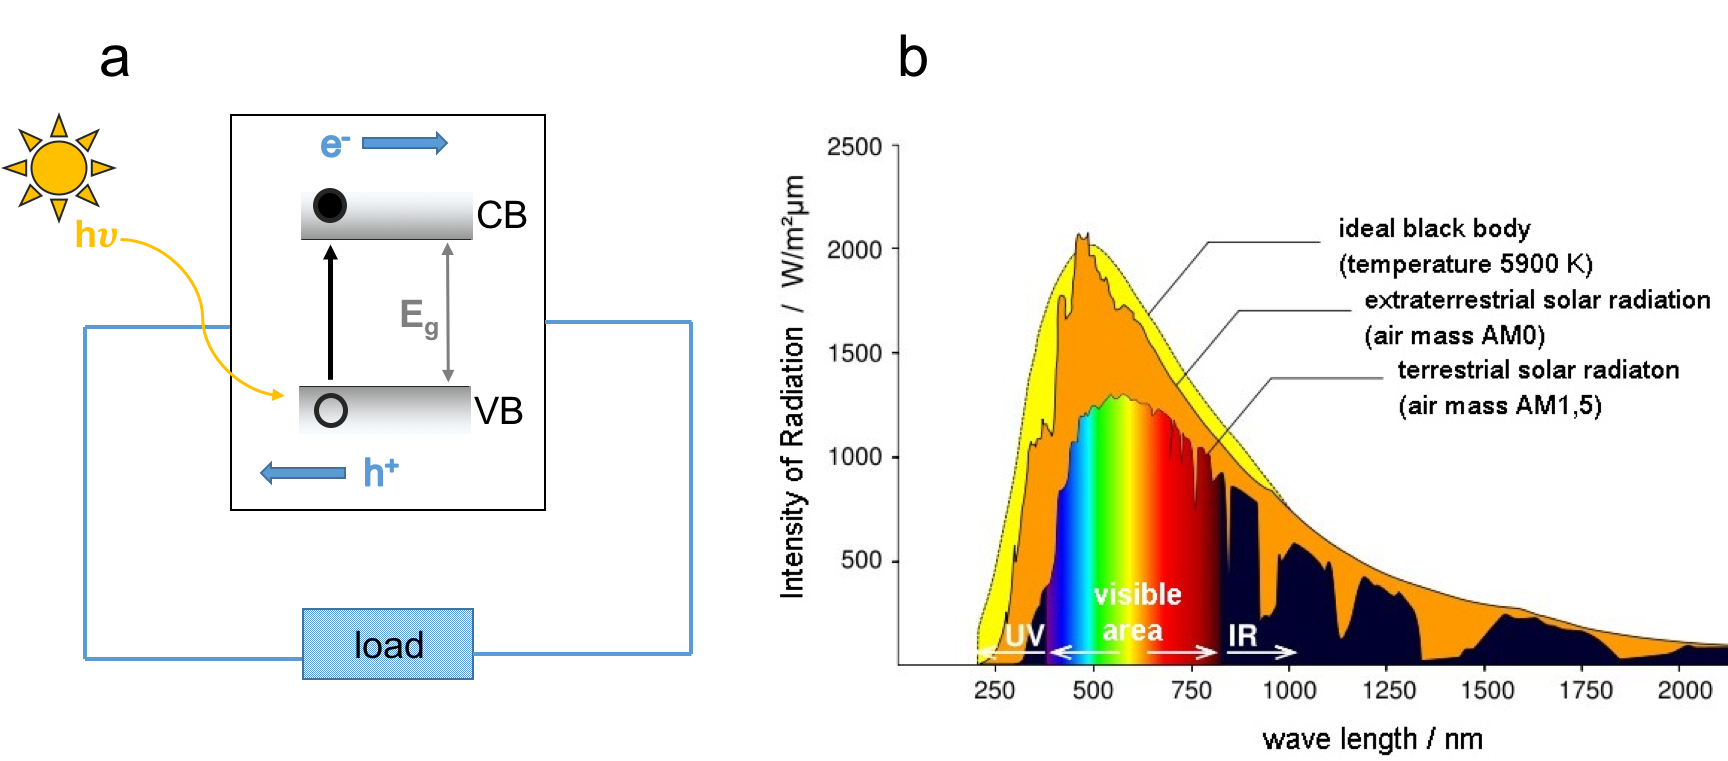
\includegraphics[width=0.95\textwidth]{figures/PV_schematic.png}
    \caption{Schematic of the photovoltaic effect: a semiconductor under illumination with some built-in electrical asymmetry to drive the separation of charge carriers to be fed into an external circuit and an external load to do electrical work (a). The AM1.5G solar spectrum, indicating the major component that is in the energy range of visible light (b). Fig. b taken from Ref. \citenum{PV_spectrum}.}
  \label{PV_schematic}
\end{figure}

In the absence of a driving force to separate the photoexcited electron and hole, the pair would quickly recombine and relax back to the ground state of the material with the emission of a photon of an energy equal to the energy of the electronic transition that has just occurred. However in a PV device, there is a `built-in' electrical asymmetry that provides an electric field to pull electrons away before they can relax and drive them towards electrical contacts to be fed into an external circuit. An electric field is effective for charge separation because it drives positively and negatively charged carriers in opposite directions \cite{Nelson5}. There are various ways to provide the electrical asymmetry, such as: through connecting a metal and a semiconductor to form a Schottky barrier junction and connecting a p-type semiconductor to an n-type semiconductor to form a p-n junction. These types of device architectures are outlined in the next section. In section \ref{ferroPVsection} novel PV phenomena in bulk materials with internal electric fields will be outlined and a search for candidate `photoferroic' materials is presented in \autoref{chap:screening}. The motivation of this investigation was to find materials where it may be possible to exploit the internal electric fields of polar crystals for enhanced local charge carrier separation.



\section{Solar cell junctions}\label{junctions}
As discussed in the previous section, an electrical asymmetry is vital for the PVE. A light absorber material must be connected to an external circuit by paths of different resistance for positive and negative charge carriers, i.e. for holes and electrons. This can be provided by spatial variation in the electronic environment, such as the junction between two electronically distinct materials.
An electrostatic field can be established by creating a junction with a gradient in the work function $\Phi_W$, electron affinity (EA) or band gap ($E_g$), which are all labelled in Fig. \ref{schottky_schematic}. The fields established by gradients in EA or $E_g$ are usually small, whereas more substantial electric fields can be achieved by a gradient in $\Phi_W$ \cite{Nelson5}.
The work function, $\Phi_W$, is the energy required to remove the least tightly bound electron from a material and is given in Eq. \ref{workfunction} where $E_{vac}$ is the energy of the vacuum level and $E_F$ is the Fermi level, which are both indicated in Fig \ref{schottky_schematic}. 
\begin{equation}\label{workfunction}
\Phi_W = E_{vac} - E_F
\end{equation}
For a metal, $\Phi_W$ is defined by the electron affinity (EA) (indicated in Fig. \ref{schottky_schematic}). For a semiconductor, $\Phi_W$ is controlled by the doping of the material, since $E_F$ within the band gap is dependant upon the doping. For instance, a semiconductor doped n-type will have $E_F$ closer to the CB and has a smaller $\Phi_W$ than if it was doped p-type. The potential difference across the junction is then the difference in the work functions of the two materials \cite{Nelson5}.
In early PV devices, the asymmetric junction was a Schottky barrier contact between a metal and a semiconductor but now more effective p-n junctions are used in solar cells, which are formed by joining together p-type and n-type semiconductors \cite{Nelson1}.
In both types of junction, the photovoltage generated is related to the difference in $\Phi_W$ of the two materials either side of the junction and the junction will develop a photovoltage provided that it presents a barrier to majority carrier currents \cite{Nelson5}. In the next sections the formation of an electrical asymmetry at a metal-semiconductor is outlined, the limitations of this type of junction in a solar cell is explained and then the formation of an electrical asymmetry at a semiconductor-semiconductor junction is outlined.

\subsubsection{Equilibrium electrical asymmetry at a metal-semiconductor junction}
\begin{figure}[h!]
  \centering
    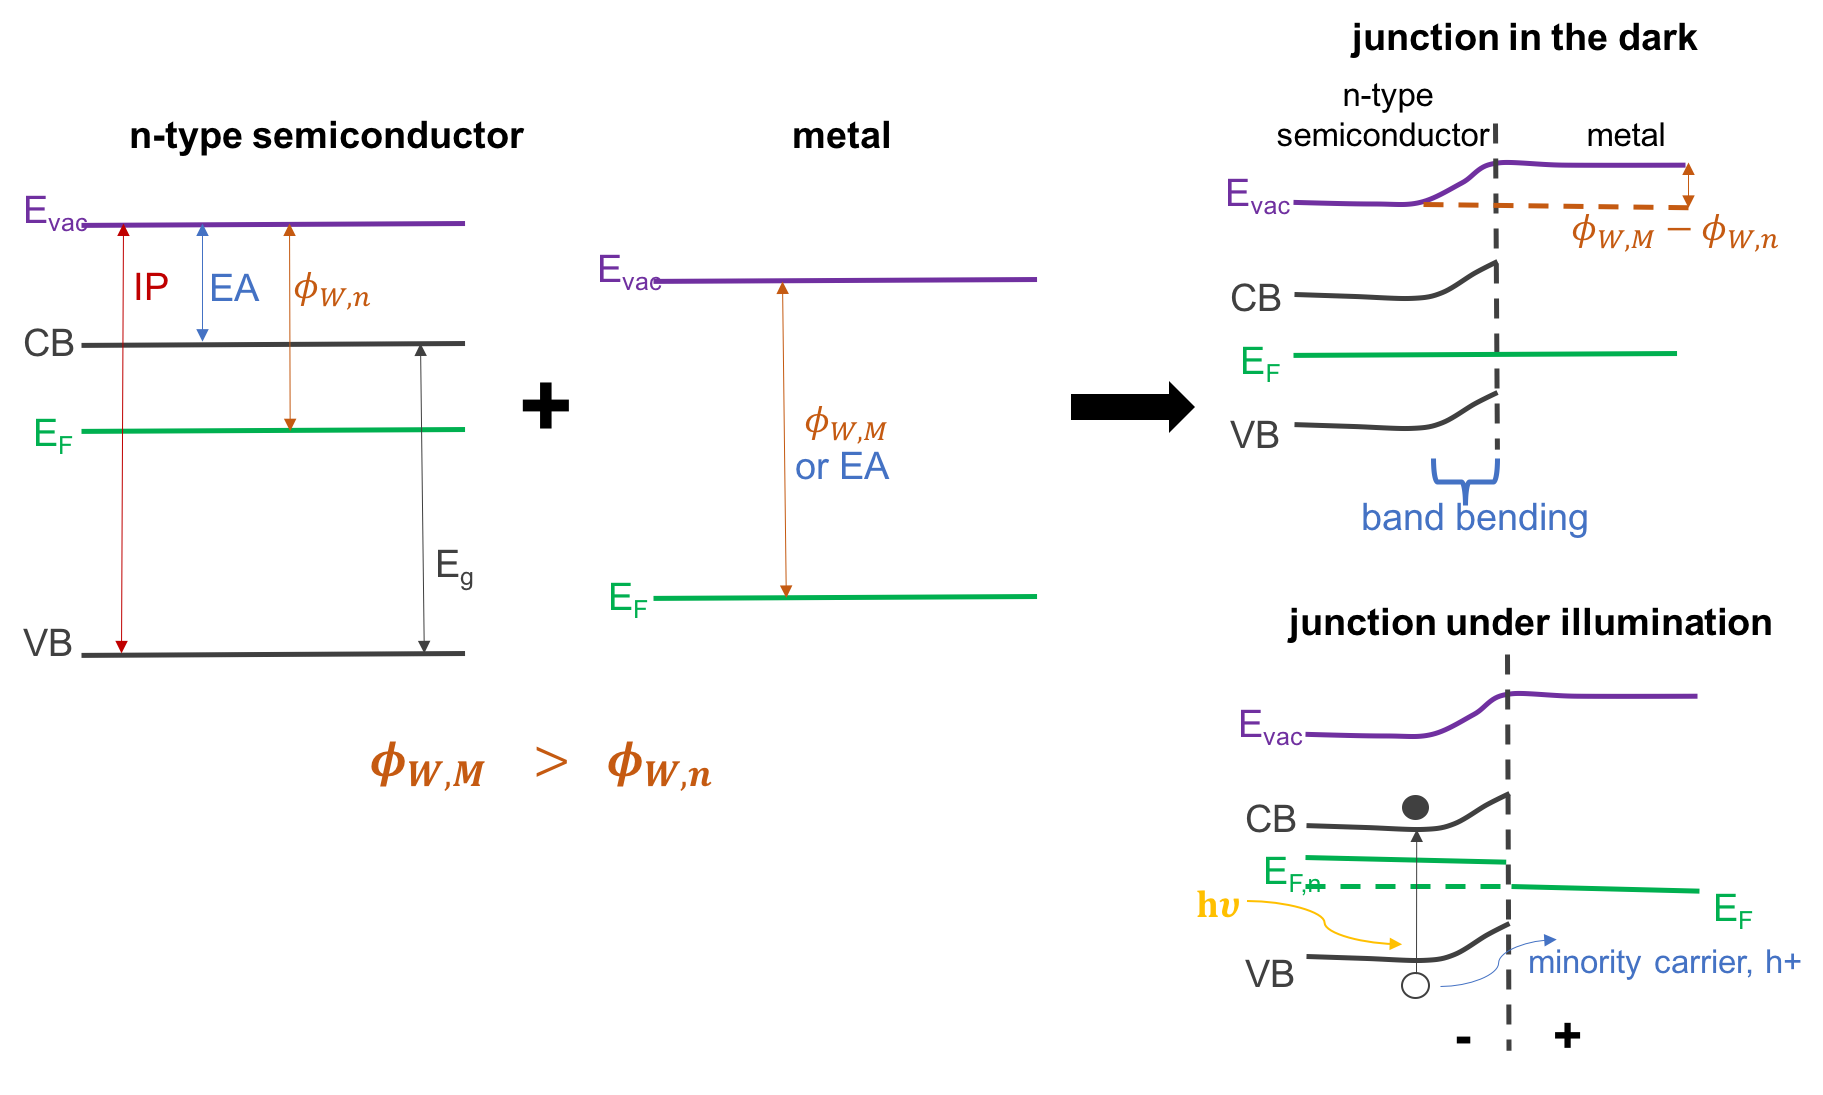
\includegraphics[width=1.0\textwidth]{figures/schottky_schematic.png}
    \caption{The formation of a Schottky barrier junction between an n-type semiconductor and a metal and the splitting of the electron Fermi level ($E_{F,n}$) under illumination. Adapted from Ref. \citenum{Nelson5} and \citenum{band_gap_rev}.}
  \label{schottky_schematic}
\end{figure}

When two materials are isolated, their $E_F$ are independent. When they are brought into electrical contact and allowed to reach thermal equilibrium there is no net current flow. Therefore by definition $E_F$ must be constant across the junction \cite{PV_bands_book}, i.e. the Fermi levels must line up as shown in Fig. \ref{schottky_schematic}. 
If the two materials have different $\Phi_W$, the vacuum level must then change between the two materials by an amount equal to the difference in $\Phi_W$ between the two materials. The electrostatic field created by a gradient in the vacuum level energy is $\frac{1}{q} \nabla E_{vac}$.
To achieve this gradient, free carriers at the junction redistribute themselves. In the case of a junction between a metal and an n-type semiconductor, if the metal has a larger $\Phi_W$ than the n-type semiconductor, electrons flow from the semiconductor to the metal. A layer of fixed positive charge in the semiconductor and a negative charge on the metal are left behind until a charge gradient builds up that is large enough to prevent any further transport of charge carriers. An electric field that still exists in a material in equilibrium is called a `built-in' electric field \cite{Nelson5}. In this case, the field would drive any excess electrons towards the positively charged side of the junction (the n-type semiconductor) and holes towards the metal side, i.e. it will provide a barrier to the flow of majority n-type carriers from the semiconductor to the metal.

As can be seen in Fig. \ref{schottky_schematic}, once the semiconductor-metal junction has formed, the CB of the bulk semiconductor is lower than that at the interface, resulting in a spatial variation in electrostatic potential towards the semiconductor-metal interface. This is the region where $E_{vac}$ is changing, the materials possess a net charge and it is called the space-charge or depletion region as it is devoid of any charge carriers \cite{PV_bands_book}. The potential is distributed across the two materials at the interface but drops off further from the interface and the electric field falls to zero.  As metals do not store charge as in a semiconductor, this distance is vanishingly small on the metal side of the junction, but on the semiconductor side this region is typically around 1 micron. The $E_g$ and EA of the semiconductor do not vary, therefore the VB and CB levels change in parallel with $E_{vac}$ at the interface, this effect is called `band bending' and the amount the bands bend is called the `built-in bias', $V_{bi}$.
In the case of a junction between a p-type semiconductor and a metal, if the metal has a smaller $\Phi_W$ than the semiconductor, the semiconductor band instead bends downwards at the interface and presents a barrier to the flow of holes from the semiconductor into the metal, which are now the majority carriers.
If instead $\Phi_W$ of the metal is larger than that of a p-type semiconductor or smaller than that of an n-type semiconductor, the bands will instead bend in such a way as to encourage majority carrier transport across the junction. Majority carriers therefore do not accumulate at the interface to develop the potential difference at the interface necessary for the PVE. This is an Ohmic contact, as opposed to a barrier. 
%Under illumination, photoexcited charge carriers pass easily across the junction and the photovoltage measured at the terminals will be negligible. 

If incident photons have an energy greater than the $E_g$ of the semiconductor in a Schottky barrier junction, then an electron-hole pair can be photoexcited (as depicted in Fig. \ref{PV_schematic}a). The system is now no longer in equilibrium as the density of electrons and holes has increased and is no longer described by the Fermi-Dirac equilibrium distribution function given in Eq. \ref{fermi-dirac}. 
The space charge region of the junction will cause the photoexcited electron-hole pair to be separated. In the case of a junction between an n-type semiconductor and a metal, electrons will accumulate in the semiconductor and holes in the metal. The semiconductor will become negatively charged and the potential difference across the junction will be reduced. $E_F$ in the semiconductor will now be different for electrons and holes, it has been split into a `quasi-Fermi level' for electrons. Far from the junction the electron quasi $E_F$ will now be larger than in the metal and larger than it was in the semiconductor before illumination, as shown in Fig. \ref{schottky_schematic}.
There are now different distribution functions for electrons in the CB and holes in the VB. It is assumed that system reaches new state of quasi-thermal equilibrium because relaxation of photoexcited electrons within the CB and holes in the VB is on a much faster timescale compared to relaxation between the bands. In each case the charge carriers are able to establish a new quasi-thermal equilibrium within the bands, with associated quasi-Fermi levels for electrons in the CB and holes in the VB, $E_{F,n}$ and E$_{F,p}$ respectively
\cite{Nelson3}.
 The illumination has generated a photovoltage equal to the difference in the Fermi level in the metal and the semiconductor \cite{Nelson5}. The quasi-Fermi level gradient can be considered as a driving force for conduction \cite{Nelson3}.

A Schottky barrier junction can therefore facilitate photovoltaic energy conversion, but it suffers from certain limitations which impact the maximum achievable photovoltages. For example, a barrier height greater than approximately half of the band gap of the semiconductor will cause minority carriers to outnumber majority carriers close to the interface region, causing an inversion layer. The junction then becomes carrier rich and cannot sustain a photovoltage. Also if the barrier region at the junction is small and the semiconductor layer is highly doped, tunneling of majority carriers across the junction may occur, reducing the effectiveness of the barrier. Many of these problems can be overcome by using a semiconductor-semiconductor p-n junction \cite{Nelson5}, outlined next.

\subsubsection{Equilibrium electrical asymmetry at a semiconductor p-n junction}
\begin{figure}[h!]
  \centering
    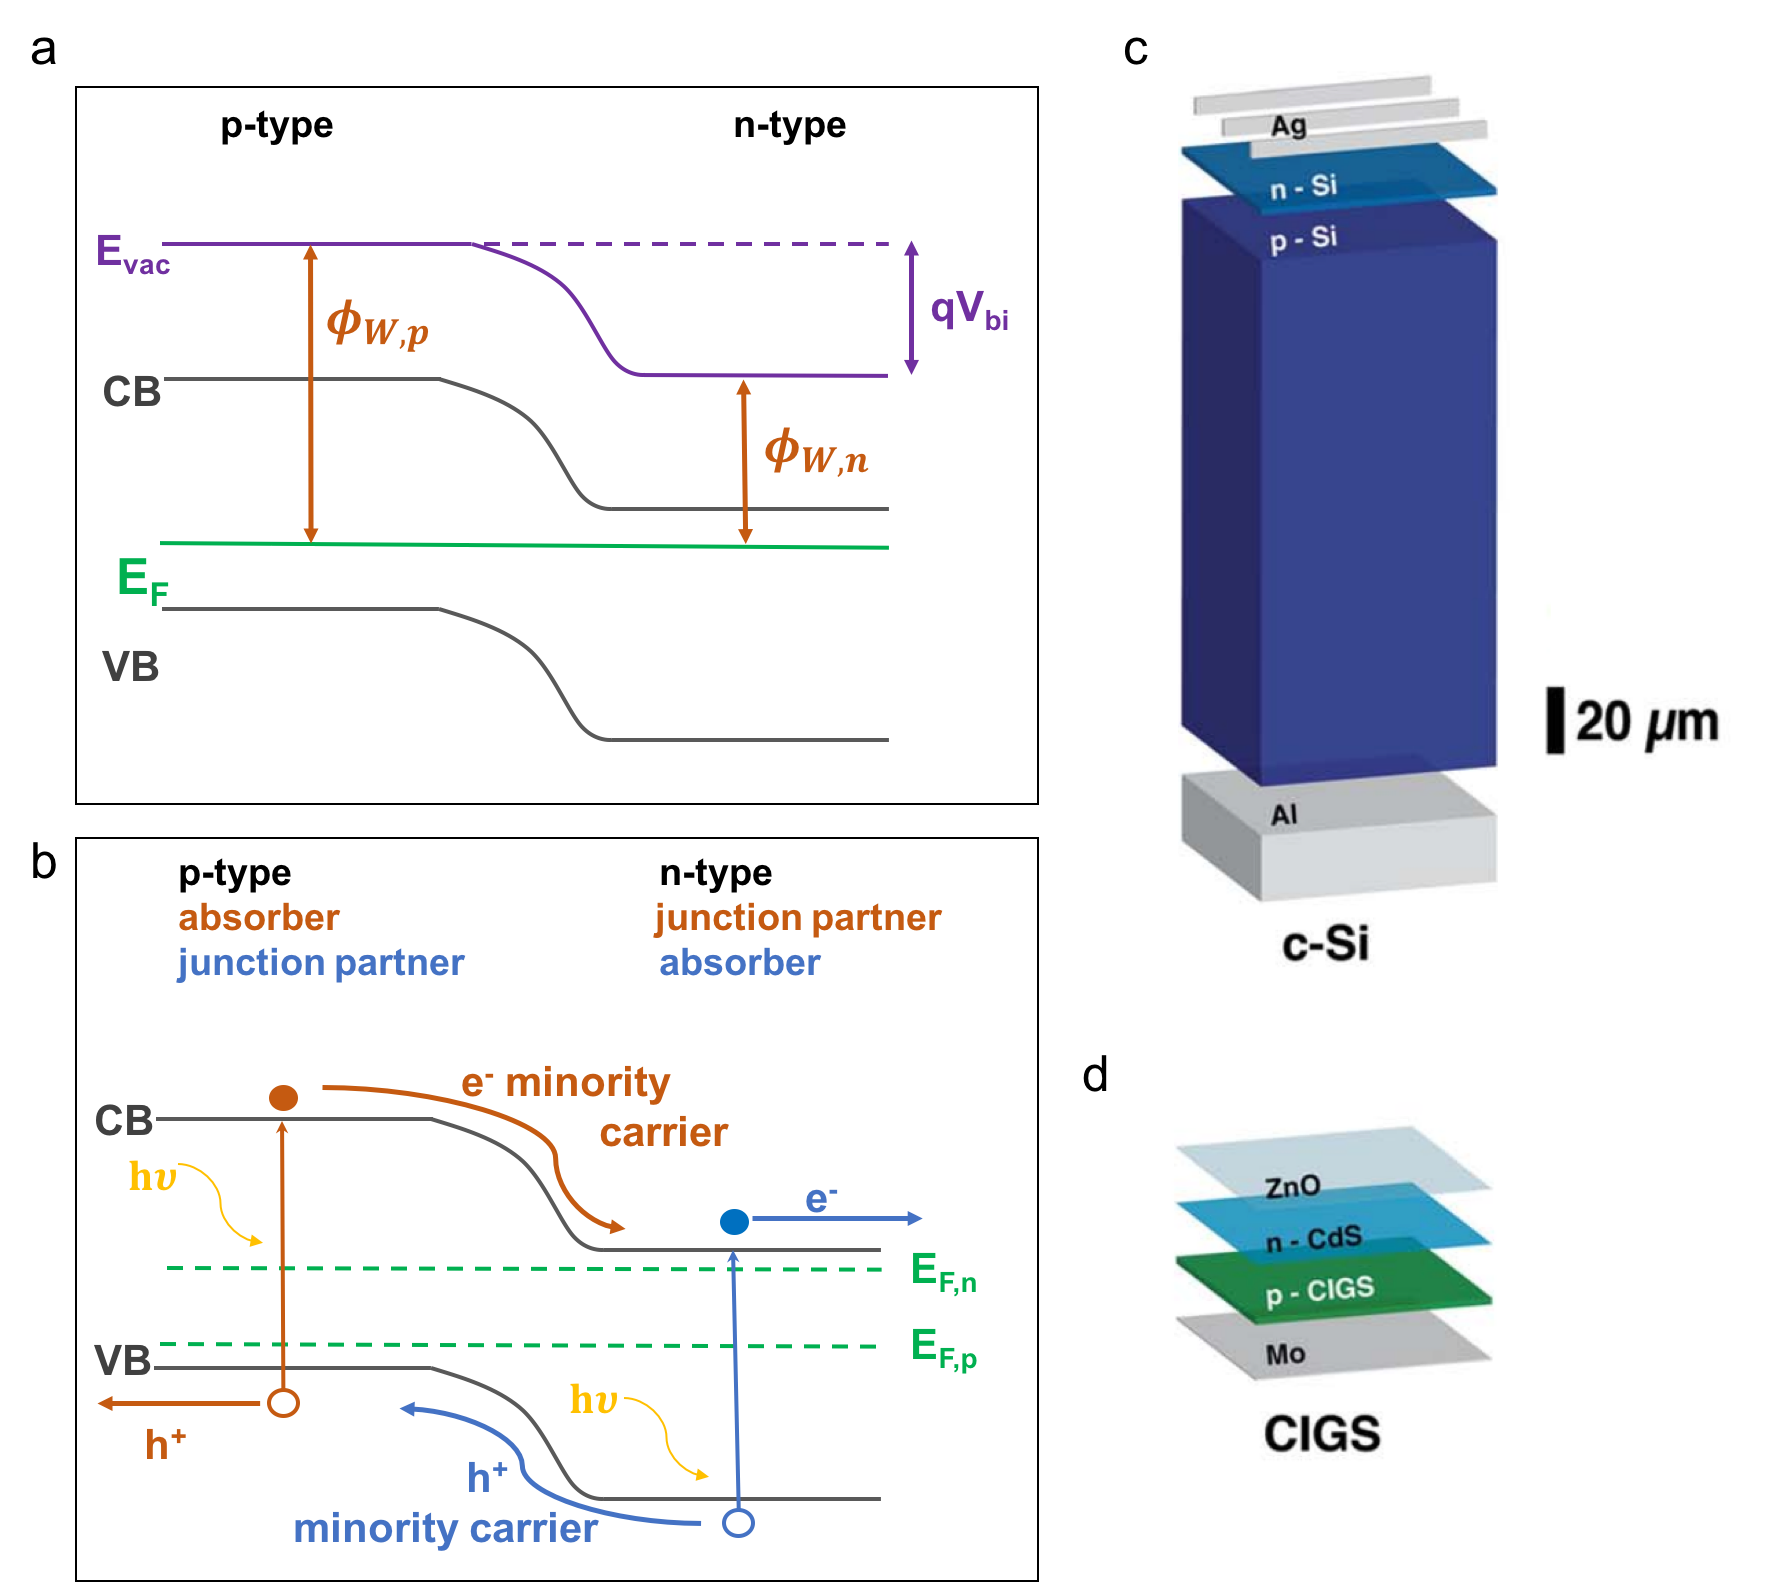
\includegraphics[width=0.85\textwidth]{figures/p-n_schematic.png}
    \caption{p-n junction formed between a p-type and n-type semiconductor, in the dark and in thermal equilibrium indicating the difference in work functions ($\Phi_W$) and built-in bias ($V_{bi}$) (a). Adapted from Ref. \citenum{Nelson5}. p-n junction under illumination indicating the direction of flow of minority carriers in the case of a p-type (orange) and n-type (blue) absorber layer (b). Adapted from Ref. \citenum{Nelson6}. Schematic of device architecture for a silicon wafer-based device (c) and a CIGS thin-film device architecture (d), both taken from Ref. \citenum{pathways}.}
  \label{p-n_schematic}
\end{figure}

For certain semiconductors, such as Si, it is possible for the material to be doped both n- and p-type depending on the valence of the dopant species relative to the host lattice, i.e. it is ambipolar. In this case, it is possible to form a junction between electrically distinct p-type and n-type semiconductors by doping different regions of the same material differently forming a `homojunction'. An example PV architecture for a Si solar cell is shown in Fig. \ref{p-n_schematic}c. Since $\Phi_W$ of the p-type is larger than that of the n-type region, an electric field is established at the junction due to the difference in electrostatic potential, as shown in Fig. \ref{p-n_schematic}a. Under illumination this will drive photoexcited electrons towards the n-type layer and holes towards the p-type layer, as shown in Fig. \ref{p-n_schematic}b. The junction region is depleted of both electrons and holes \cite{Nelson5}.

%In real, non-ideal, solar cell devices power is dissipated through parasitic resistances in the device, including current leakage and resistance from the electrical contacts \cite{Nelson1}. In the case of the p-n junction architecture shown schematically in Fig \ref{PV_architecture}b, there can be series resistance of the p and n layers to the flow of majority carriers, resulting in a reduction in the potential between the junction and the terminal. There can also be resistance at the contact layers in the device, such as those indicated in Fig. \ref{PV_architecture}c and \ref{PV_architecture}d \cite{Nelson6}. The open circuit voltage (V$_{OC}$) of a device can be reduced by non-ideal alignment of the electronic bands of the different layers within the device. 
For many of the materials being studied for use as absorber layers in thin-film solar cells, such as chalcogenide-based materials like the device shown in Fig. \ref{p-n_schematic}d, it is not possible, or is very difficult, to achieve ambipolar doping \cite{band_alignment_review, Zhang_doping_limits}. Therefore to achieve a p-n junction for many thin-film PV devices it is necessary to form an interface between two different materials with different energy gaps, lattice constants and even slightly different crystal structures. Due to such mismatches, defects are expected to be more prevalent at heterojunction interfaces than at homojunction interfaces. In section \ref{sulfosalt_band_alignment} band alignments that have been proposed for reducing the impact of defects at p-n heterojunctions will be discussed and suggestions for p-n junction partners for the candidate photoferroic solar absorber materials are presented.

\section{Photoferroic phenomena}\label{ferroPVsection}
% ** Cite Rappe about shift current (+BPE?) possible in any crystal that lacks centre of inversion symmetry, not just FE materials
A ferroelectric material possesses a spontaneous electric polarisation that can be switched between two or more states using an electric field \cite{new_FE_PV_1}. Many interesting PV phenomena have been observed in ferroelectric (FE) materials such as the bulk photovoltaic effect (BPE) and the anomalous photovoltaic effect (APE) \cite{keith}. 
%Ferroelectric materials usually have a high dielectric constant (which was mentioned in section \ref{PV_properties} as an important parameter for a photovoltaic material) and they possess a spontaneous electric polarization that can be switched between two or more states using an electric field \cite{new_FE_PV_1}.
The BPE was first recorded in 1956 in BaTiO$_3$ \cite{keith_46}, where photovoltages were measured in un-doped single crystals \cite{keith}.
The BPE effect is distinctly different from the typical PV effect in semiconductor
p-n junctions outlined in section \ref{junctions} as the driving force for the photocurrent is provided by the internal electric polarisation of the crystal \cite{FE_PV_rev1}. 
The APE was first observed in PbS films in 1946 \cite{keith_54} and has since been reported in polycrystalline CdTe, ZnTe, InP \cite{keith_55, keith_56, keith_57}, where photovoltages output along the polarisation direction can be significantly larger than the band gap of the material \cite{FE_PV_rev1}, which is usually the limit for a semiconductor PV material \cite{keith}. 
The Shockley-Queisser limit \cite{SQ_1961}, which prevents any single p-n junction solar cell from converting more than 33.7\% of the incident light into electricity, has not been predicted to apply for these photovoltaic phenomena. An upper limit for the theoretical power conversion efficiency (PCE) from this photovoltaic mechanism seems to still be an open question \cite{ FE-PV_kirchartz, new_FE_PV}, although an ultimate maximum efficiency of any single-band gap absorber of 44\% has been set by thermodynamic considerations \cite{SQ_1961}. 

The identification, understanding and utilisation of such phenomena discussed above may open up the possibility of more efficient PV devices constructed from photoactive-ferroelectric, i.e. `photoferroic', materials.
In addition to the above novel PV effects, it has been proposed that the presence of electric polarisation in a PV absorber material may allow for efficient polarisation-driven charge carrier separation \cite{Jarv, FE-PV_lett} and also that ferroelectric materials in solar cells may allow for control over the internal electric fields and carrier injection barriers, which play a central role in the PV mechanism \cite{FE-PV_kirchartz}.
However, most of the commonly used ferroelectric materials such as LiNbO$_3$ and BaTiO$_3$ have band gaps larger than 3 eV and can therefore only absorb sunlight in the UV range to convert into electricity, which accounts for only around 3.5\% of the solar spectrum. Research efforts have sought to adjust the optical absorption of ferroelectric materials without influencing the ferroelectric properties through chemical doping or alloying \cite{FE_PV_rev1}. In Bi$_4$Ti$_3$O$_{12}$ the optical band gap has been tuned in such a way, resulting in a decrease from 3.6 eV to 2.7 eV \cite{FE_PV_rev1_83}, although this is still considerably larger than the optimal range for a PV absorber material, as discussed in section \ref{PV_properties}. A recent study has demonstrated a more substantial reduction in the optical band gap of BaTiO$_3$  to 1.66 eV, whilst maintaining 70\% of the original polarisation \cite{FE-PV_lett}, however the PV performance of the modified material was not demonstrated in this study. 

This then leads on to the second component of this study: to identify new candidate solar absorber materials that may exhibit ferroelectricity and have band gaps within the optimal range for the absorption of sunlight. The screening criteria used to identify these candidate absorber layers will be outlined further in \autoref{chap:screening}, but the basic principles are as follows: by starting from a dataset of naturally occurring minerals, it could be assumed that all candidates are likely to be thermodynamically stable. Secondly, necessary (although not sufficient) conditions are used to screen for candidate photoferroic materials. A dark streak colour for the mineral implies that the magnitude of the optical band gap may be somewhere within the visible spectrum and therefore within the ideal range for a PV absorber layer. A polar space group is a necessary, but again not sufficient, condition for a material to exhibit ferroelectricity. Even in the absence of switchable ferroelectric states, the internal crystal polarisation may be beneficial for a PV material, as mentioned earlier.
The optoelectronic properties of the candidate materials are then investigated further to assess the likely performance of solar cells made from these absorber materials to determine those worthy of further experimental study. The identification of stable materials with a large polarisation and strong optical absorption could provide more test systems for further experimental investigation and, ideally, the development of control of the novel FE-PV phenomena outlined at the start of this section.


\section{Absorber material properties for efficient solar cells}\label{PV_properties}
The most fundamental, necessary requirement for a solar absorber material in a PV device is that it possesses a band gap across which an electron can be excited. As discussed in the previous section, the magnitude of this band gap must also be somewhere within the energy range of the solar spectrum so that sunlight can induce this excitation. The next most fundamental requirement of a solar absorber material is that it must allow for the transport of charge carriers out of the absorber material layer, into a collection electrode and on to an external circuit in order to do electrical work. Provided these necessary conditions are met and some sort of spatial asymmetry (outlined above) is present to drive electrons away from their point of promotion, the material should exhibit the PVE \cite{Nelson2}. However, how well it will actually peform in a solar cell is determined by more stringent criteria and other material properties. 

Firstly the actual value of the band gap within the range of the solar spectrum (shown in Fig. \ref{PV_schematic}b) is of importance. It is ideal for the value to be as close as possible to the region of photon energies that make up the majority of the solar spectrum. The optimal range for the band gap under typical radiation conditions is approximately 1.0 to 1.7 eV \cite{PV_E_range}. The upper limit of the power conversion efficiency (PCE) of incident photon energy into electrical energy by a device made from a particular absorber material based on its band gap was first calculated by Shockley and Quiesser in 1961 \cite{SQ_1961}. A plot of theoretical efficiency limit as a function of band gap was shown in figure \ref{SQ}, as well as the record efficiencies of various PV technologies.

\begin{figure}[h!]
  \centering
    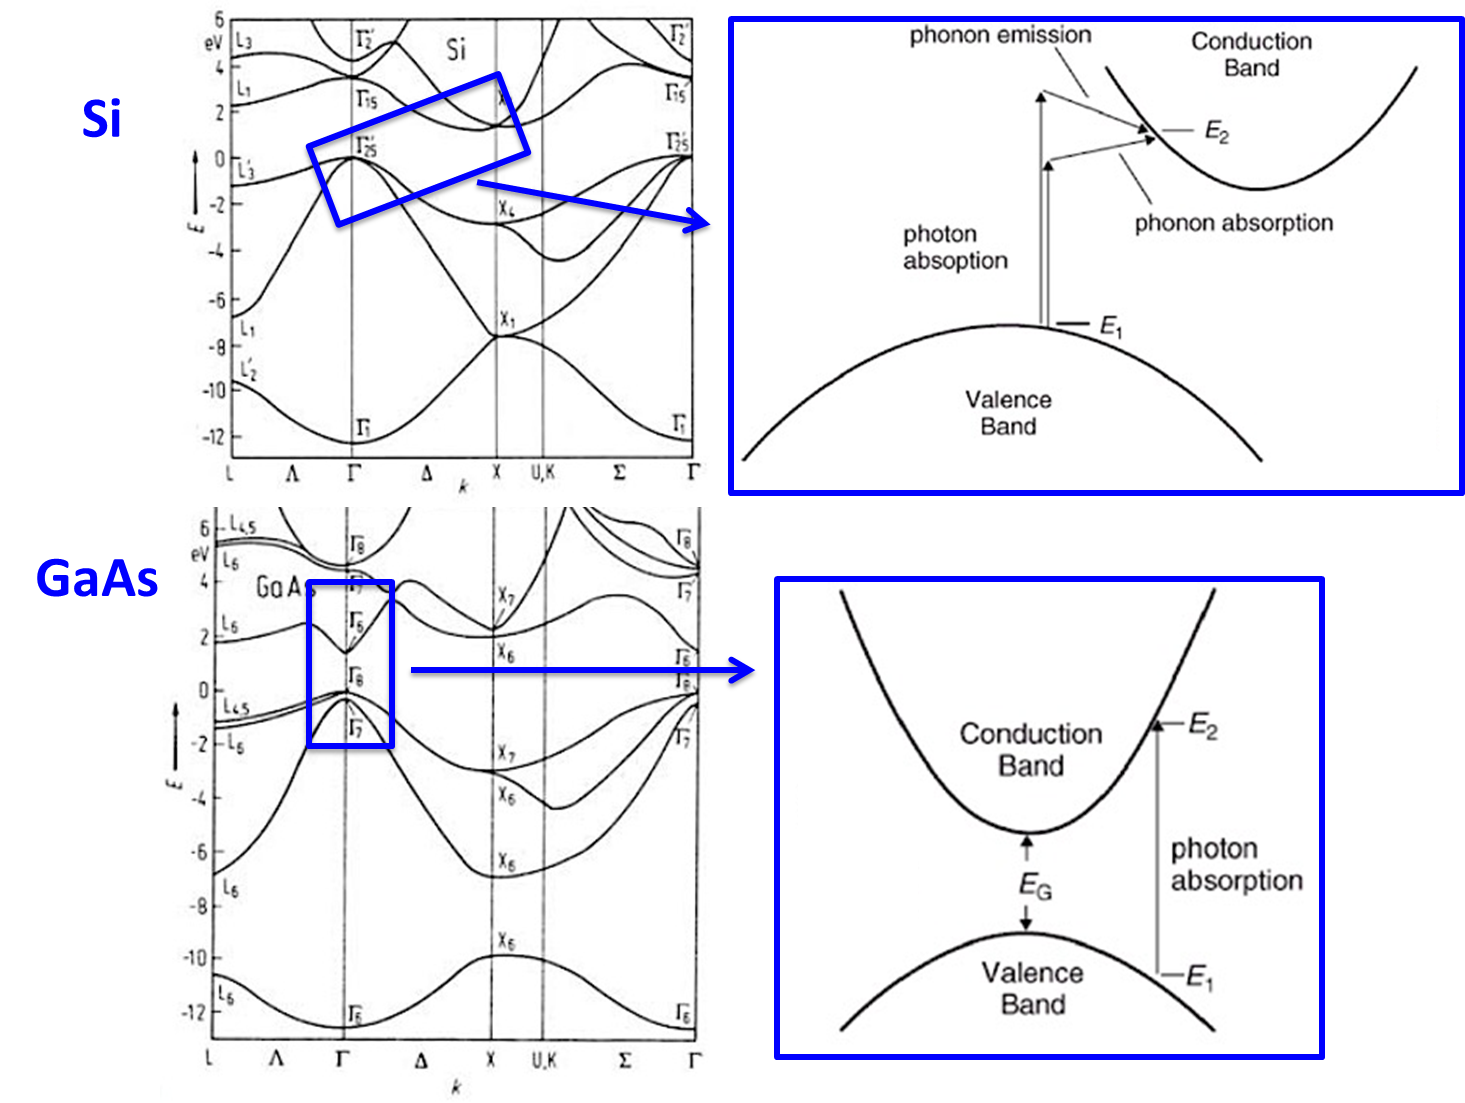
\includegraphics[width=0.95\textwidth]{figures/Si_and_GaAs.png}
    \caption{The band structure of silicon and a schematic of the absorption process in an indirect band gap semiconductor (top). The band structure of GaAs and schematic of the absorption process in a direct gap semiconductor. Figures adapted from \citenum{phys_semicond} and \citenum{PV_bands_book}.}
  \label{Si_and_GaAs}
\end{figure}

However, it is not only the value of the band gap that is of importance. More intricate details of the band structure of the material can also impact on the performance of a solar cell device made from the material. Whether the band structure shows a band gap that is direct or indirect can have an impact on the performance of a solar cell made from the material. Figure \ref{Si_and_GaAs} shows the band structures of Si and GaAs, where Si possesses an indirect band gap and GaAs possesses a direct band gap, i.e. the extrema of the VB and CB occur at the same value of \textbf{k} for the latter but not for the former. The excitation of an electron from the valence band maximum to the conduction band minimum is called fundamental absorption, as there are several other optical absorption transitions that can occur in a semiconducting material, especially in a defective material, and this point will be discussed more in section \ref{defects_impact}. Both the total energy and momentum of all particles involved in the absorption process must be conserved. Photons do possess momentum ($\frac{h}{\lambda}$), however this is very small compared to the range of crystal momenta and so the electron momentum is effectively conserved during photon absorption. For a direct transition, the absorption coefficient of a material for a given photon energy $h \nu$ is proportional to the probability, p$_{12}$, of the transition of an electron from the initial state E$_1$ to the final state E$_2$, the density of electrons in the initial state, $g_{v}(E_1)$, and the density of available final states, $g_{c}(E_2)$. This is then summed over all possible transitions between states where $E_2 - E_1 = h\nu$. Since the electron momentum is conserved during a direct transition, the crystal momentum in the valence band is approximately the same as that of the final state in the conduction band at energy $E_2$ \cite{PV_bands_book}.

However for an indirect band gap semiconductor, such as silicon shown at the top of figure \ref{Si_and_GaAs}, the valence band maximum occurs at a different crystal momentum to that of the conduction band minimum. As discussed earlier, the momentum of a photon is far less than that of crystal momenta. In order to conserve the momentum of an electron during an optical transition across an indirect band gap, momentum must be either provided by the lattice or released to the lattice usually in the form of the particle representation of a lattice vibration, known as a phonon, as indicated in the top right schematic of figure \ref{Si_and_GaAs}. Since both a phonon and an electron are needed to make an indirect transition possible, the optical absorption coefficient, $\alpha$, depends not only on the density of states of the electrons, as for a direct transition, but also on the availability of emitted or absorbed phonons with the required momentum. Therefore, $\alpha$ for an indirect transition compared to a direct transition is typically relatively small and more heavily dependent on temperature \cite{Nelson3}. 

\begin{figure}[h!]
  \centering
    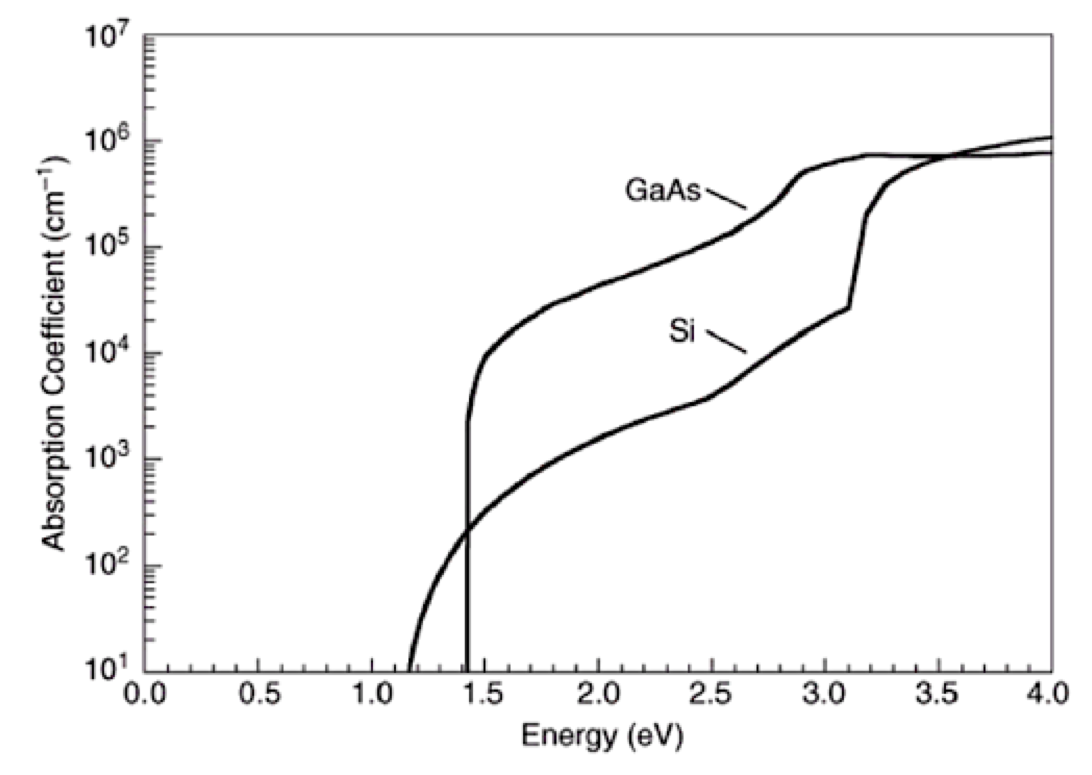
\includegraphics[width=0.8\textwidth]{figures/absorption_fig2.png}
    \caption{A comparison of the absorption coefficients of the indirect band gap semiconductor Si and the direct band gap semiconductor GaAs across a range of incident photon energies. Figure taken from reference \citenum{PV_bands_book}.}
  \label{absorption_fig2}
\end{figure}

$\alpha$ of a material determines the penetration depth, $\frac{1}{\alpha}$, of light incident on the material \cite{absorption_coeff_book1}. Fig. \ref{absorption_fig2} shows the absorption coefficients of different semiconductors across a range of wavelengths. The figure shows a less steep onset of absorption for silicon, which as discussed earlier possesses an indirect band gap, compared to that of GaAs for which the absorption corresponds to a direct band-to-band transition. 
The implication of the differing $\alpha$ and therefore different optical penetration depths of absorber layers is that materials which are stronger absorbers require less material to absorb the light. This forms the basis of thin-film solar cell technologies.
On the other hand materials with a weaker onset of absorption, as is often the case for materials with an indirect band gap such as Si, a thicker layer of absorber material is required to absorb the same amount of light \cite{PV_bands_book}. This is undesirable if the particular material contains rare or expensive components and also results in higher demands on material quality as charge carriers must be transported through the absorber material in order to be collected.
Thin-film PV technologies typically require a less high-quality and defect-free absorber layer as charge carriers do not have to travel through as much of the material in order to reach a collection electrode. However, defects in the absorber layer do still play a decisive role in determining the device performance of thin-film film PV technology, and this point is discussed much more in section \ref{defects_impact}.

\begin{figure}[h!]
  \centering
    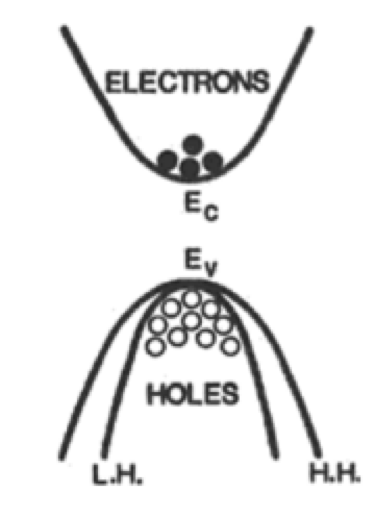
\includegraphics[width=0.2\textwidth]{figures/heavy_holes.png}
    \caption{Schematic of a the band structure of a photoexcited semiconductor with electrons near the bottom of the conduction band, holes near the top of the valence band, where the particular material has both heavy- and light-hole bands (labelled H.H and L.H in the figure respectively). Figure taken from reference \citenum{heavy_holes}.}
  \label{heavy_holes}
\end{figure}

As mentioned in section \ref{BandTheorySection}, another property of importance that can be derived from the band structure of a material is the effective mass, m*. m* is related to the curvature of the band at the top of the valence band (for holes) or at the bottom of the conduction band (for electrons). The m* of electrons or holes are the masses they seem to carry for transport properties \cite{dielectric_const1}. For example, in ZnSnO$_3$ the hole m* has been calculated to be large, indicating that hole mobility will be poor in this material. Poor mobility will make carrier extraction difficult, which has been linked to the low photocurrents observed in this material \cite{effective_mass1}. m* are calculated by fitting a formula to the band extrema when using the parabolic approximation. However, just from a quick inspection of the band structure of a material, a more steeply curved shape to the band extrema indicates a lower effective mass and therefore satisfies a necessary condition for higher carrier mobility. Fig. \ref{heavy_holes} shows a schematic of the band structure of a direct band gap semiconductor that has both heavy- and light-hole bands at the valence band extremum, where the flatter band corresponds to the heavy-hole band.
%Although certain thin-film technologies, which will be discussed towards the end of section \ref{current_tech}, reduce the amount of absorber material the charge carrier must travel through before being collected. So although carriers must still travel through the material, effective mass could be considered less of a crucial parameter for this technology. 
However m* should just be considered as a necessary but not a sufficient condition for good carrier mobility as the effect of the effective mass on the transport properties could be overshadowed by scattering of charge carriers by defects in a real, non-ideal material. 

\section{Impact of absorber layer defects on solar cell performance}\label{defects_impact}
%Refer to: pg 160 \cite{fund_semi}, pg 51, 52, 64 \cite{thin_film_Boer}, pg 63 + 65 \cite{phys_semicond}\\
Although the main framework for modeling solid-state systems (as outlined at the start of this chapter) is built around perfect, periodic systems; in reality absolutely perfect systems do not exist. Deviations from the perfect crystal lattice structure (i.e. defects) can strongly influence the performance of electronic devices. There is an energy cost associated with the creation of a defect, but in many cases the free energy of a system can be lowered by the incorporation of a certain concentration of defects due to an increase in the configurational entropy of the system \cite{AshcroftMermin_general}. Methods for modeling defects in solids are discussed in section \ref{defects_methods}, but here the impact of defects in the absorber layers on the performance of solar cells is discussed.

There are many different possible types of crystal defect. If a defect does not involve any atoms that are foreign to the host crystal, then the defect is called an intrinsic or native defect. Defects involving foreign atoms, or impurities, are referred to as extrinsic defects. Fig. \ref{defects}b and \ref{defects}c show some examples of extrinsic and intrinsic defects. This work is primarily interested in the fundamental material properties of candidate solar absorber materials, so only intrinsic defects are considered. In real systems however, impurities are sometimes unintentionally present in the growth or processing environment.
Defects are usually classified as point or extended defects. Point defects usually involve isolated atoms in localised regions of a host crystal, such as those shown in Fig. \ref{defects}b and \ref{defects}c. There are a number of different possible point defects, such as: vacancies, interstitials and antisites, which correspond to the removal, insertion or substitution of species from the perfect host lattice respectively. Extended defects may involve rows of atoms, such as a dislocation defect. An example of a line defect is shown in figure \ref{defects}a. Another possible type of defect is a defect complex, which is composed of a small number of point defects.

\begin{figure}[h!]
  \centering
    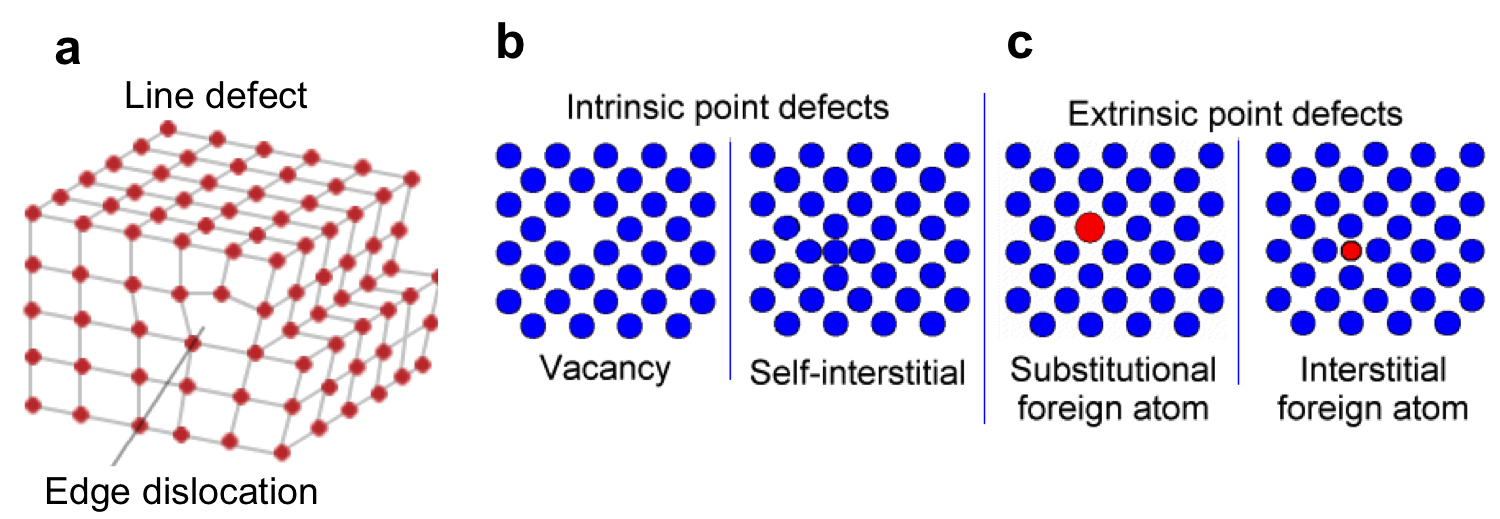
\includegraphics[width=0.9\textwidth]{figures/defects.png}
    \caption{An example of a line defect (a) and both intrinsic (b) and extrinsic (c) point defects. Figures taken from references \citenum{defects_fig1} and \citenum{defects_fig2} respectively.}
  \label{defects}
\end{figure}

The electrical properties of semiconductors can be modified significantly by the incorporation of very small amounts of impurities or defects. It is often the case that less than one defect per million of host atoms is sufficient to alter the properties of a semiconductor \cite{fund_semi}. This sensitivity to defects is one of the reasons why semiconductors find many uses in device applications. For example, luminescence centres in wide-band-gap materials can be used to emit light at specific wavelengths or single-spin centres provided by defects can act as artificial atoms and serve as a qubit in a quantum computer \cite{defects_tutorial}. In order to control the electrical properties of a material by introducing defects, typically processes must first be developed to produce a fairly defect-free material, before intentionally introducing particular defects \cite{fund_semi}. In the case of solar cell devices, however, the presence of defects can be detrimental depending on the nature of the defect \cite{Aron_defect_tolerance}, which will be discussed next. 

Certain point defects result in additional energy levels in between the valance-band maximum (VBM) and conduction-band minimum (CBM), i.e. within the band gap of the material. Electrically active defects have at least one charge state for the defect that produces a defect level in the band gap. This level then has an associated defect wavefunction, a state to which the electron is added to or removed when the charge state of the defect changes. If the defect level is positioned close enough to the band edges such that the defect is likely to be thermally ionised at room temperature, then the defect is conventionally referred to as a `shallow'. If the defect produces a level in the band gap and far from the band-edge, it is a referred to as `deep'.  Another way of defining a defect as `shallow' or `deep' is based on the degree of localisation of the wavefunction. If a defect wavefunction is delocalised (on the order of many lattice constants) then the defect has the characteristics of a shallow defect. If the wavefunction is instead localised on the length scale of an atomic bond then this indicates a deep level defect \cite{defects_tutorial}. 

Typically deep levels are thought to be the most detrimental to solar cell device performance \cite{Stoneham_killer_defects}. 
Defects that produce mid-gap states act as Shockley-Read-Hall recombination sites \cite{SRH}, which is regarded as the most important recombination process in real, non-perfect semiconductors. It is a form of non-radiative recombination where a charge carrier is trapped in the defect state before recombining with a charge carrier of opposite polarity. This type of recombination is known to be detrimental to device performance as, essentially, it results in energy input from sunlight not being converted into electricity \cite{Nelson4}.
In the case of {\CZTS}, predictions for the defect formation energy and defect levels in reference \citenum{defects_Chen} suggest that defects which would be expected to produce a deep defect level, also have a high formation energy so would be expected to be less likely to form.
However, a recent theoretical study has revisited the defect physics of {\CZTS} to demonstrate that similar detrimental effects may also be possible with some shallower defects \cite{Sunghyun_killer_defects}.

The energy band model described in section \ref{BandTheorySection} has been successful in explaining many aspects of the behaviour of solids and a large amount of experimental data has supported the theoretical predictions made using the model. Its main drawback however is that it assumes a perfect, or nearly perfect, crystal lattice. It applies well to single crystals and polycrystalline substances, but omits important physical characteristics when used to study materials that are amorphous or heavily disordered so that the structure deviates significantly from the periodicity of the crystal \cite{small_semiconductor1}.
Low concentrations of impurities and defects can be modeled by considering, for example, the introduction of distinct additional donor and acceptor energy levels within the band gap of a material and the scattering of electrons and holes in the solid. However, in {\CZTS} the presence of a large extent of disorder amongst Cu and Zn, and hence high concentrations of $Cu_{Zn}^{-}$ and $Zn_{Cu}^{+}$ antisites, has been inferred from calculations of defect formation energy \cite{defects_Chen} and confirmed from experiment \cite{Schorr, CZTS_Xray, CZTS_TEM}. 
At higher defect concentrations, defect levels interact to form a band. For example, for high n-type doping the impurity band merges with the conduction band, causing a rigid shift of the conduction band towards the valence band \cite{Pankove}. The band profile can be modified with increasing donor density as shown in figure \ref{bs2}a-c. 
%to give rise to conductivity even at temperatures that are too low to produce excitation of carriers into the free conduction bands, called impurity band conduction \cite{small_semiconductor2}.
In heavily-doped semiconductors it is possible to observe a phenomena called `band tailing', where the valence and conduction bands are shifted towards each other resulting in a narrowing of the band gap, as shown in figure \ref{bs2}d \cite{Pankove}. The heavy-doping effects then result in a different emitted spectrum which can be detected by techniques such as photoluminescence (PL) spectroscopy. 

\begin{figure}[h!]
  \centering
    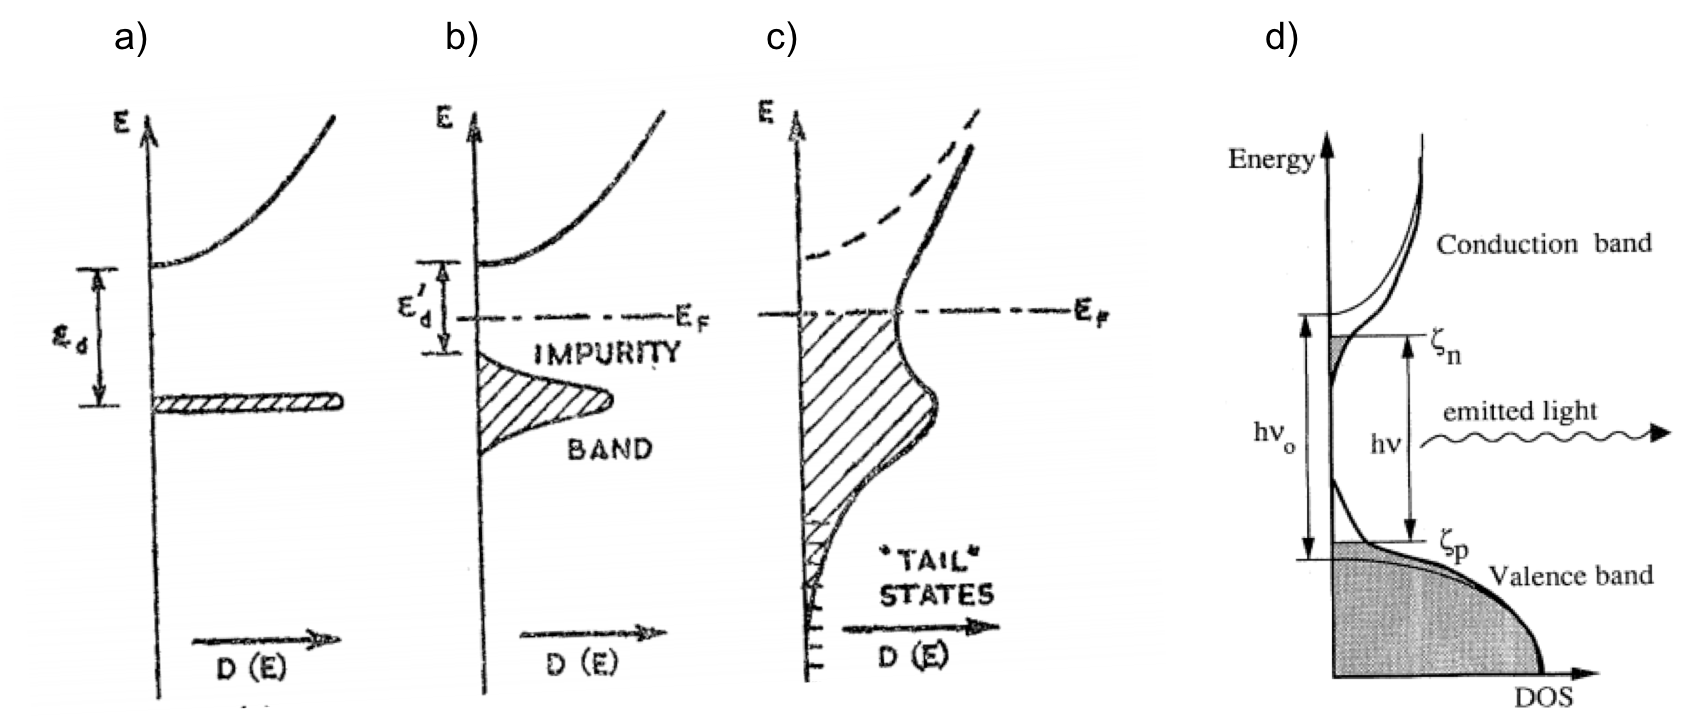
\includegraphics[width=0.9\textwidth]{figures/bs2+pankove.png}
    \caption{The influence of increased donor impurity density on the conduction band profile showing low (a), medium (b) and high (c) densities of impurities. Figure taken from reference \citenum{small_semiconductor2}. (d) Schematic of band tailing. $\zeta_{n,p}$ are the quasi-Fermi level for electrons and holes respectively. The narrow line denotes the unperturbed density of states (DOS), while the heavy line depicts the DOS modified by heavy-doping effects. Both valence and conduction bands are shifted towards each other to give a narrowing of the band gap and the DOS is distorted, showing band tails. Figure taken from reference \citenum{Pankove}.}
  \label{bs2}
\end{figure}

%\begin{figure}[h!]
%  \centering
%    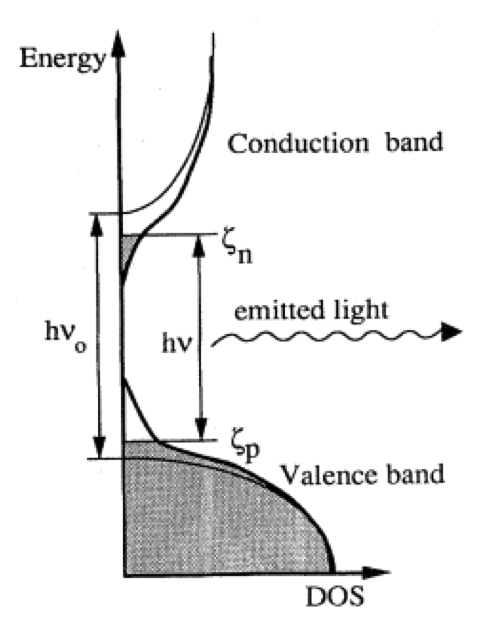
\includegraphics[width=0.4\textwidth]{figures/pankove_band_tailing.png}
%    \caption{Schematic of the laser operation at T=0 K in GaAs. $\zeta_{n,p}$ are the quasi-Fermi level for electrons and holes respectively. The narrow line denotes the unperturbed density of states (DOS), while the heavy line depicts the DOS modified by heavy-doping effects. Both valence and conduction bands are shifted towards each other to give a narrowing of the band gap and the DOS is distorted, showing band tails. Heavy doping effects result in a different emitted spectrum. Figure taken from reference \citenum{Pankove}. **CONDENSE FIGURES**}
%  \label{pankove_band_tailing}
%\end{figure}

In a PL experiment, photons with energies larger than that of the band gap excite electrons from the valence band to the conduction band, as shown in figure \ref{PL_transitions}a. In addition, electrons can be excited from or to defect levels, as shown in figure \ref{PL_transitions}b. When the excited electrons transition to lower energy levels, they can emit light to conserve energy, resulting in a peak in the PL spectrum. In a photoluminescence excitation (PLE) experiment, the PL intensity is measured as a function of excitation photon energy. This gives an absorption profile for the defect. PL measurements are able to pick up optical signatures of defects even if they are only present at low concentrations with high resolution. PL measurements alone however cannot be used to identify the character of a defect, this is an area where first-principles defect calculations can provide some insight \cite{defects_tutorial}. 

\begin{figure}[h!]
  \centering
    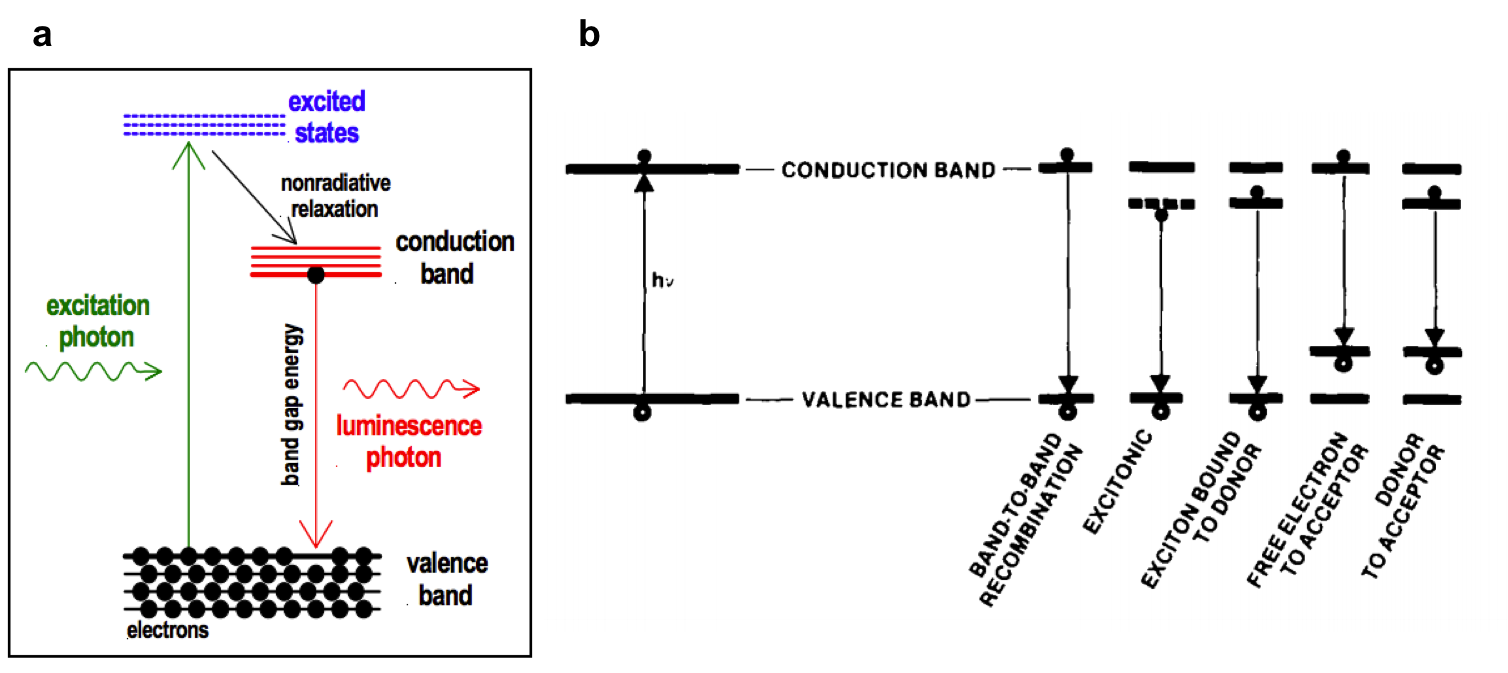
\includegraphics[width=1.0\textwidth]{figures/PL_transitions.png}
    \caption{Basic optical transitions involved in a measurement during photoluminescence spectroscopy (a). Common emission transitions detected during photoluminescence measurements, including transitions involving defect levels (b). Figures taken from reference \citenum{PL_transitions} and \citenum{Pankove} respectively.}
  \label{PL_transitions}
\end{figure}

Several PL studies have been performed on kesterite-structured samples of {\CZTS}, Cu$_2$ZnSnSe$_4$ and alloys of the two. PL measurements have been performed on both full devices and polycrystalline thin-films \cite{band_tail, Gershon, Gershon_ref18, Romero, Miyamoto, Unold} and single crystals \cite{Halliday, Levcenko, Hones}. Reference \citenum{Halliday} compares the PL spectra for varying compositions of the sample, whereas in reference \citenum{band_tail} measurements on both CIGSSe and record-efficiency CZTSSe thin films are performed in an attempt to account for the difference in the performance of these two technologies by comparing their defect-influenced PL emission spectra. Polycrystalline samples are more similar to those likely to be used in thin-film CZTS photovoltaic devices, however comparison between those measurements with single crystal measurements could enable the isolation of recombination at grain boundaries and interfaces from those due to defects in the bulk of the absorber layer. 
%Also measurements performed on single crystals as close to perfectly stoichiometric {\CZTS} as possible are likely to be the most directly relatable to our simulations on bulk systems. 
One feature common to all of the PL spectra from studies on kesterite samples is clear evidence of defects and disorder from the observed band tailing. 
Fig. \ref{CZTS+CIGS_PL} shows photoluminescence (PL) spectroscopy measurements performed on CZTSSe thin films by Gokmen et al \cite{band_tail}. The figure shows that there is a shift in the PL peak to lower energies (red-shifting), below the value of the band gap obtained from internal quantum efficiency (IQE) measurements performed on the same thin films. It is also noted in this study when comparing the PL spectra of CZTSSe films to that of CIGSSe films that the PL peak for CZTSSe thin films is broader and that the red-shifting was roughly twice as severe. This effect is referred to as the `band-edge tailing', where photons of energies less than the band gap of the material are emitted following photoexcitation and subsequent relaxation back to the ground state. 
%This effect is known to be detrimental for device performance as emitted photons may then not have sufficient energy for subsequent photoexcitations in the absorber layer, the energy of the original photon may then not be converted into electricity if the photoexcited electron-hole pair recombine before the charge is collected \cite{Nelson4}.
%The PL spectra of kesterite samples usually features a much broader peak than that observed in CIGSSe samples, such as that shown in figure \ref{CZTS+CIGS_PL}. The energy of the maximum PL peaks of kesterite samples is also usually considerably red-shifted compared to the energy of the band gap. These two features are usually attributed to band tailing caused by either spatial band gap variations or electrostatic potential fluctuations in the absorber material.  Both effects lead to a non-zero density of states (DOS) within the band gap \cite{culprit, band_tail}. 
Measurements performed in reference \citenum{band_tail} found the tailing in CZTSSe to be roughly twice as severe as that observed in higher-performing CIGSSe devices.


\begin{figure}[h!]
  \centering
    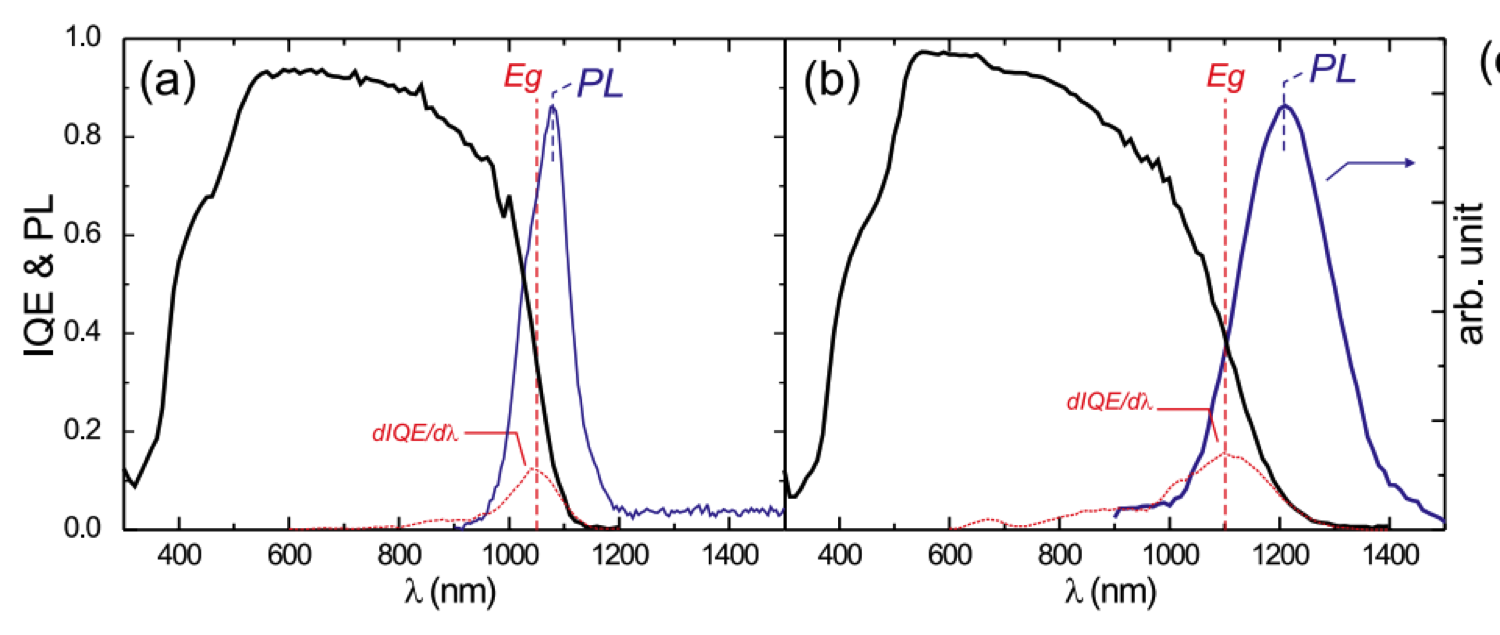
\includegraphics[width=1.0\textwidth]{figures/CZTS+CIGS_PL.png}
    \caption{The internal quantum efficiency (IQE), band gap as determined from the IQE inflection point and the photoluminescence spectra of high performance devices with thin-film absorber layers of (a) CIGSSe (E$_g$ = 1.19 eV) and (b) CZTSSe (E$_g$ = 1.13 eV). Figure taken from reference \citenum{band_tail}.}
  \label{CZTS+CIGS_PL}
\end{figure}

\begin{figure}[h!]
  \centering
    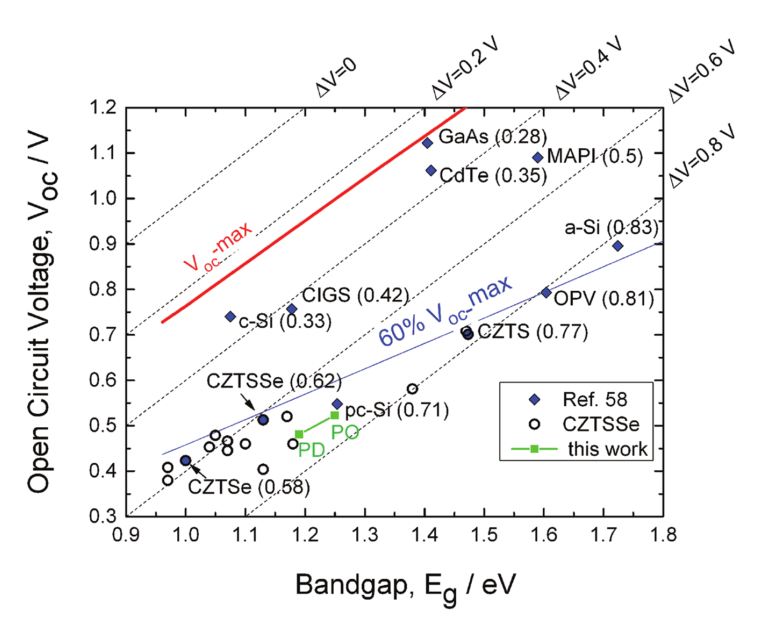
\includegraphics[width=0.75\textwidth]{figures/Voc.png}
    \caption{V$_{OC}$ versus band gap of high performance CZTSSe devices ($>$9\% efficiency) indicated by circles with best devices based on other photovoltaic materials shown for comparison by diamond symbols: Methyl-ammonium lead iodide (MAPI), amorphous silicon (a-Si), organic photovoltaic films (OPV), crystalline silicon (c-Si) and polycrystalline silicon (pc-Si). The oblique lines give a constant V$_{OC}$ deficit from 0.8 V to 0 V. The green points correspond to CZTSSe films that are partially ordered (PO) or partially disordered (PD) due to disorder amongst Cu and Zn. Figure taken from reference \citenum{culprit}.}
  \label{Voc}
\end{figure}

The low open circuit voltage (V$_{OC}$) relative to the band gap has been recognised as the key limiting factor on the performance of {\CZTS} solar cells \cite{culprit}. 
The measured current density-voltage (J-V) curve of a solar cell is used to determine the solar to electric power conversion efficiency (PCE), $\eta$. The PCE of a solar cell is the ratio of power output from the solar cell ($P_{MP}$) to the power input from the Sun ($P_{in}$). This is shown in Eq. \ref{PV_efficiency}. $P_{MP}$ is given in terms of the V$_{OC}$ (the voltage from the J-V curve of the solar cell at J = 0) and the short-circuit current density, $J_{SC}$, (the current density on the J-V curve at V = 0) in Eq. \ref{P_MP}.
For an efficient solar cell, it is desirable to have a high $J_{SC}$, a high $V_{OC}$ and a FF that is as close to 1 as possible.
\begin{equation} \label{P_MP}
P_{MP} = FFV_{OC}J_{SC}
\end{equation}
\begin{equation} \label{PV_efficiency}
\eta = \frac{P_{MP}}{P_{in}} = \frac{FFV_{OC}J_{SC}}{P_{in}}
\end{equation}
As can be seen from the position of CZTSSe devices on the plot in figure \ref{Voc}, the open circuit voltages measured for these devices are considerably less than that of the higher-performing CIGS devices, which have a similar value for the band gap of the material.
In general, the main cause of V$_{OC}$ deficit in a PV device is the recombination of photogenerated charge carriers in the bulk material or at surfaces \cite{culprit}. In {\CZTS} one explanation that has been put forward is band tailing in the bulk \cite{band_tail}.


\begin{figure}[h!]
  \centering
    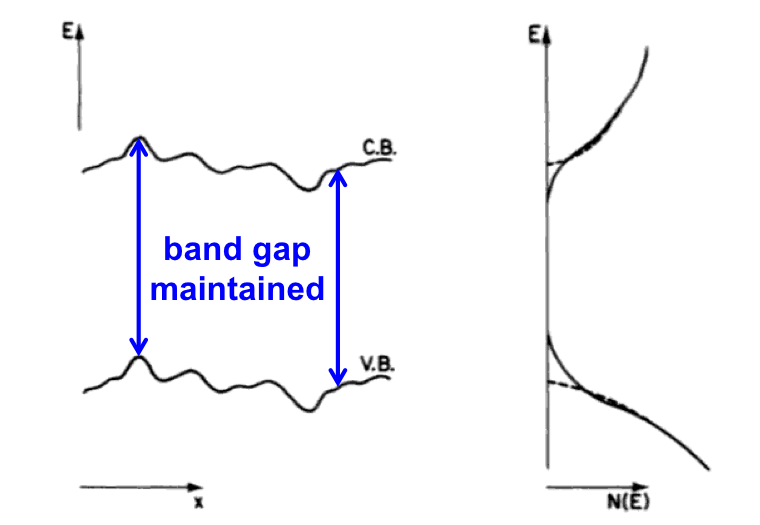
\includegraphics[width=0.6\textwidth]{figures/pankove_elec_fluc.png}
    \caption{The perturbation of the band edges by Coulomb interaction with inhomogeneously distributed impurities (left), leading to the formation of tail states (right). Dashed lined show the distribution of states in the unperturbed case. Figure taken from reference \citenum{Pankove} and adapted.}
  \label{pankove_elec_fluc}
\end{figure}

\begin{figure}[h!]
  \centering
    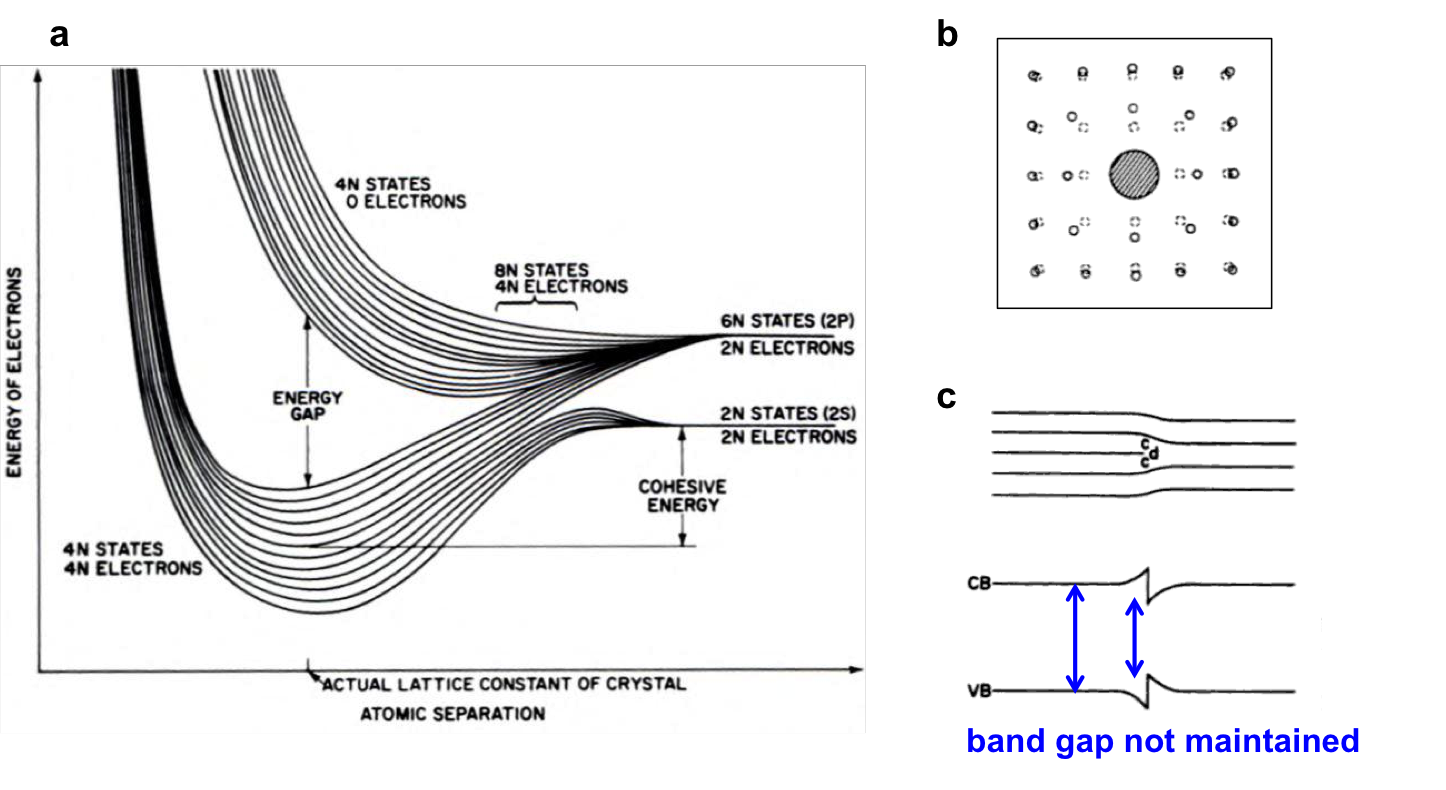
\includegraphics[width=1.0\textwidth]{figures/pankove_band_fluc.png}
    \caption{Energy banding of allowed levels in diamond as a function of spacing between atoms (a). Compressional strain induced in a crystal lattice by the incorporation of a large impurity atom (b). Deformation potential in the band structure due to compressional and dilational strain from an edge dislocation defect (c). Figures taken from reference \citenum{Pankove} and adapted.}
  \label{pankove_band_fluc}
\end{figure}

Observed band tailing can be caused by either spatial band gap variations or electrostatic potential fluctuations in the material \cite{band_tail}. In the case of the latter, it is the inhomogeneous distribution of ionised defects that cause the fluctuations. An ionised donor exerts and attractive force on conduction electrons and a repulsive force on valence holes. As the defects are distributed randomly, the local interaction varies depending on the crowding of the defects. In this case the energy gap between the valence band and conduction band is maintained, as shown in figure \ref{pankove_elec_fluc} and the states of each tail are spatially separated \cite{Pankove}. Defects can also result in fluctuations in the band gap of a material. For example, if an impurity atom is of a different size to the atoms of the host lattice, then this can result in a local mechanical strain, as shown in figure \ref{pankove_band_fluc}b which results in a deformation potential, such as that shown in figure \ref{pankove_band_fluc}c for an edge dislocation defect. Local strains can alter the separation of atoms in the crystal and, as figure \ref{pankove_band_fluc}a shows, the atomic separation within a crystal has a significant impact on the band structure. Additionally, due to the narrow region of phase stability for {\CZTS}, it is also possible there may be compositional inhomogeneity and secondary phases present \cite{SandS}, which could also produce local band gap fluctuations. 

In \autoref{chap:CZTS} of this work, a Monte Carlo model is developed to allow for the investigation of the possible contribution to band tailing in {\CZTS} from the potential fluctuations of high concentrations of $Cu_{Zn}^{-}$ and $Zn_{Cu}^{+}$ antisites. In section \ref{sulfosalt_defects} we perform electronic structure calculations for point defects to investigate the defects physics of candidate `photoferroic' solar absorber materials for which no experimental measurements have yet been made.



\chapter{Methodology}

\section{Electronic structure calculations}\label{elec_struc}
%See Richard Martin book (Ch1), etc. \cite{RichardMartin_Ch1}

\subsection{Quantum theory of materials}

%** See Prasad ch1 (intro) + ch2 for SE\\

The properties of materials are determined by their constituent electrons and nuclei and how they interact with each other. Nuclei are massive (compared to electrons) and can usually be described using classical mechanics with interactions via Coulomb's law. However, as hypothesised by de Broglie in 1924 and later demonstrated experimentally by Davisson and Germer and also by Thomson with electron diffraction, electrons exhibit wave-like behavior in addition to particle-like behavior and do not obey classical mechanics \cite{quantum_intro}. The behaviour of the electrons largely determines the physical and chemical properties of a material \cite{Prasad_ch2}, such as the bonding that holds the material together and many of the observed macroscopic properties such as the optical, electrical and magnetic properties \cite{RichardMartin_Ch1}. But to describe the behaviour of electrons, it is necessary to use quantum mechanics.

Quantum mechanical systems can be described by the Schr{\"o}dinger equation, which describes the energy of the electrons and nuclei within a material where electrons interact with the positively charged atomic nuclei through an electrostatic potential \cite{Lesar}. The time-dependent Schr{\"o}dinger equation for a one-electron system is given in equation \ref{SE}, where the first term on the left hand side of the equation is related to the electron's kinetic energy, the second term to the electron's potential energy and $\psi$ is used to denote the one-electron wavefunction.
\begin{equation} \label{SE}
\left( - \frac{\hbar^2}{2m} \nabla^2 + \hat{V} \right)\psi(r,t) = i\text{ } \hbar\frac{\partial \psi(r,t)}{\partial t}
\end{equation}
In section \ref{BandTheorySection} the one-electron Schr{\"o}dinger equation for an electron moving in a weak periodic potential with the nearly free electron approximation was used to discuss obtaining the energy eigenvalues of the electron as a function of \textbf{k}, i.e. the electronic band structure of a periodic, crystalline solid.
However, for systems containing more than one electron we must consider the many-body Schr{\"o}dinger equation and this soon becomes a very complex problem. This is due to the many electrons in the system interacting with each other as well as with the nuclei. The Schr{\"o}dinger equation for a system containing M nuclei and N electrons is shown in equation \ref{many_SE} \cite{Lesar}, where uppercase \textbf{R} denotes nuclear coordinates and lowercase \textbf{r} denotes electron coordinates. This is a very complex mathematical problem for most systems. For example, the many-body wavefunction, $\Psi$, in equation \ref{many_SE} for 1 cm$^3$ of a typical metal would be a function of approximately $10^{23}$ variables.

\begin{multline}  \label{many_SE}
\left\{ - \frac{\hbar^2}{2m} \left( \frac{\nabla_{n_1}^2}{m_1} + ... + \frac{\nabla_{n_M}^2}{m_M}, 
\frac{\nabla_{e_1}^2}{m_e} + ... + \frac{\nabla_{e_N}^2}{m_e} \right)
+ V \left( \mathbf{R_1},...,\mathbf{R_M}, \mathbf{r_1}, ..., \mathbf{r_N} \right)
\right\}
\Psi (\mathbf{R_1},...,\mathbf{R_M}, \mathbf{r_1}, ..., \mathbf{r_N}, t) \\
= i\hbar \frac{\partial\Psi(\mathbf{R_1},...,\mathbf{R_M}, \mathbf{r_1}, ..., \mathbf{r_N},t)}{\partial t}
\end{multline}

When dealing with such systems, the Born-Oppenheimer approximation is almost universally used. As electrons are fast moving relative to the nuclei, they are considered to be moving in the classical field generated by static nuclei. This decouples the nuclear and electronic degrees of freedom, allowing us to separate the ionic and electronic wavefunctions. 
%The total energy of the system is now just the sum of the energy of the electrons and the nuclei and only the electronic density requires quantum mechanical treatment. 
When using the Born-Oppenheimer approximation it is also assumed that nuclear motion cannot cause electronic transitions, therefore the electrons will remain in their ground state. There is now no explicit time dependence for the electron density as electrons are assumed to always be in their ground state for the instantaneous ionic configuration and that they transition adiabatically to their ground state for each ionic configuration. This approximation is generally more suitable for semiconductors than for metals as phonon energies are usually less than the energy of the electronic band gap in a semiconductor and hence ionic motion cannot excite electrons to higher energy states \cite{Prasad_ch2}. $\Psi$ for electrons in the system is now no longer a function of t and so it is the solution of the time-independent Schr{\"o}dinger equation for the system of ions and electrons that is of interest and the ionic system can be considered separately from the electronic system which is subjected to the classical electric field of a stationary ionic system.
%and is only a function of electron coordinates (lowercase r in Eq. \ref{many_SE}).

The general form of a time-independent Schr{\"o}dinger equation for the electronic system is shown in Eq. \ref{TISE}, where H is the Hamiltonian operator used to determine the total energy of a system with the wavefunction $\Psi$. Lowercase \textbf{r} are the electronic coordinates and $\sigma$ is used to denote the spin of electrons, which was omitted in earlier equations for simplicity. The Born-Oppenheimer Hamiltonian for the electrons is shown in Eq. \ref{Born-Opp}, where l are the ionic sites, Z is the nuclear charge, m is the electron mass, i is the index of the electron and j are the indices of all other electrons in the system. The first term is the kinetic energy of the electrons, the next terms are related to the potential energy of the electrons. The second term is the Coulomb attraction between electrons and static nuclei and the third term is the Coulomb repulsion between different electrons \cite{Prasad_ch2}.
\begin{equation}\label{TISE}
H\Psi(\mathbf{r_1}, ..., \mathbf{r_N}, \sigma_1, ..., \sigma_N) = E\Psi(\mathbf{r_1}, ..., \mathbf{r_N}, \sigma_1, ..., \sigma_N)
\end{equation}
\begin{equation}\label{Born-Opp}
H = - \sum_i \frac{\hbar^2}{2m}\nabla_i^2 - \frac{1}{4 \pi \epsilon_0}\sum_i \sum_l \frac{Ze^2}{|\mathbf{r_i}-\mathbf{R_l}|} + \frac{1}{8 \pi \epsilon_0} \sum_{ij, i \neq j}\frac{e^2}{|\mathbf{r_i}-\mathbf{r_j}|}
\end{equation}
Although we can write out the electron Hamiltonian as shown above, we do not know the exact form of the many-body wavefunction in Eq. \ref{TISE}. The third term in the expression for the Hamiltonian, the summation of electron-electron interactions in the system, is the cause of a dramatic rise in computational expense as the system size (and hence number of interacting electrons) increases. In the next section various approaches that have been developed to treat electron-electron interactions are outlined and those utilised in this work are highlighted.

%\subsection{History of electronic structure theory}

\subsection{Treatments of electron-electron interactions}

\subsubsection{Approximations of the many-body wavefunction}
As we do not know the exact form of the many-body wavefunction, $\Psi$, the simplest way to avoid the dramatic rise in complexity with increased system size from electron-electron interactions in the many-body Schr{\"o}dinger equation is to approximate the form of $\Psi$ to allows us to decouple electron-electron interactions. In the `independent particle approximation', as used in the Hartree method, electrons are treated as independent and are included in an average electron-electron interaction scheme. The method involves assuming approximate forms of both the Hamiltonian and the many-body wavefunction. The electron-electron interaction term in the Hamiltonian in Eq. \ref{Born-Opp} is replaced by one that accounts for only the repulsion between an electron and the average position of all other electrons, the electrons therefore interact with an average effective potential instead of many, many interactions between all pairs of electrons in the system. This is an example of a mean field approximation.
%The second term in  Eq. \ref{Born-Opp} is then combined with the modified electron-electron interaction term to form an effective potential, the Hartree potential (V$_{eff}$). 
As electrons are considered to be independent, the many-body wavefunction can be written as the product of single-electron wavefunctions (or orbitals) as shown in Eq. \ref{Hartree}, where $\psi_i(\mathbf{r_i}, \sigma_i)$ is the wavefunction of a single electron i at position $r_i$ with spin $\sigma_i$ \cite{Prasad_ch2}. 
\begin{equation}\label{Hartree}
\Psi_H = \psi_1(\mathbf{r_1}, \sigma_1) \psi_2(\mathbf{r_2}, \sigma_2) ... \psi_N(\mathbf{r_N}, \sigma_N)
\end{equation}
To solve the many-body Schr{\"o}dinger equation, the Hartree method pioneered the self-consistent field method \cite{RichardMartin_Ch1}. Firstly, the variational principle is invoked to set up an inequality for the groundstate energy, $E_0$, of the system (i.e. the minimum total energy) to find an approximate value of $E_0$ and the corresponding set of $\psi_i$. This is shown in Eq. \ref{var_princip} where the middle term is the expectation value of a state of the system described by the many-body wavefunction $\Psi$. Many properties of interest can be determined from $E_0$ of the system and from changes in the energy of the system in response to particular perturbations. $E_0$ can be used to determine various structural properties such as equilibrium bond lengths, surface configurations and the most likely defect structures in a material.
\begin{equation}\label{var_princip}
E = \braket{\Psi | H | \Psi } \geq E_0
\end{equation}
The solution of the Hartree equation, shown in Eq. \ref{Hartree_eq}, depends on the Hartree potential, shown in Eq. \ref{V_Hartree}, but the potential depends on the solution of the Hartree equation itself to obtain $\psi_i$. The solution of the Hartree equation therefore involves a self-consistent procedure. A guess is made for $V_H(\mathbf{r})$ and then Eq. \ref{Hartree_eq} is solved. Then the solution is used to calculate $V_H(\mathbf{r})$ with Eq. \ref{V_Hartree} and the Hartree equation is solved again with this new value for $V_H(\mathbf{r})$. The procedure is repeated until input and output potentials are the same, within a given tolerance \cite{Prasad_ch2}.
\begin{equation}\label{Hartree_eq}
\left[ -\frac{\hbar^2}{2m_e}\nabla^2 + V_I(\mathbf{r}) + V_H(\mathbf{r}) \right] \psi_i(\mathbf{r}) = \epsilon_i \psi_i(\mathbf{r})
\end{equation}
\begin{equation}\label{V_Hartree}
V_H(\mathbf{r_i}) = \frac{1}{4 \pi \epsilon_0} \int \frac{d^3r}{|\mathbf{r_i} - \mathbf{r}|}e^2 \sum_{j \neq i} |\psi_j\mathbf{r}|^2
\end{equation}
\begin{equation}\label{V_I}
V_I(\mathbf{r_i}) = -\frac{1}{4 \pi \epsilon_0} \sum_l \frac{Ze^2}{|\mathbf{r_i} - \mathbf{R_l}|}
\end{equation}

There are however a number of large drawbacks of the Hartree method. The mean-field approach to obtaining the Hartree potential is flawed due to spurious self-interaction of an electron interacting with itself as it is also included in the average electron density it interacts with when calculating the electron-electron interaction term.
The next large omission of the Hartree method is electron correlation. The probability of finding an electron at $\mathbf{r_1}$ is uncorrelated to finding one at $\mathbf{r_2}$ because it can be written as a product of two one-electron probabilities. Paraphrasing John Perdew from his talk at the 2015 `Hands-on workshop density-functional theory and beyond: First-principles simulations of molecules and materials' helps to explain why this is neglecting some behaviour of the electron density: electron correlation can be likened to shoppers at a busy shopping mall where many people are moving around but in such a way that they try to avoid bumping into each other. Neglecting this effect can lead to results as unphysical as the dissociation of the H$_2$ molecule \cite{Prasad_ch2}.

Lastly, the basic Hartree method described above does not account for electron exchange. Although the spin of the electron is included in Eq. \ref{Hartree}, it actually plays no role in the Hartree method. The many-body wavefunction needs to be antisymmetric under particle exchange as required by the Pauli Exclusion Principle for fermions. This requirement is shown in Eq. \ref{antisym}. According to the Pauli Exclusion Principle, no two fermions can occupy the same quantum state. The spin quantum number therefore should be taken into account. The Hartree-Fock (H-F) extension to this method is able to account for this latter flaw \cite{Prasad_ch2}.
\begin{equation}\label{antisym}
\Psi(\mathbf{r_1}\sigma_1, ..., \mathbf{r_i}\sigma_i, ..., \mathbf{r_j}\sigma_j, ...) = - \Psi(\mathbf{r_1}\sigma_1, ..., \mathbf{r_j}\sigma_j, ..., \mathbf{r_i}\sigma_i, ...)
\end{equation}
The requirement shown in Eq. \ref{antisym} can be satisfied by using the Slater determinant as the trial wavefunction, as shown in Eq. \ref{Slater_det}, where N is the number of electrons.
\begin{equation}\label{Slater_det}
\Psi(\mathbf{r_1}\sigma_1, ..., \mathbf{r_N}\sigma_N) = \frac{1}{\sqrt{N!}} \begin{bmatrix}
\psi_1(\mathbf{r_1}\sigma_1) & \psi_1(\mathbf{r_2}\sigma_2) & \dots & \psi_1(\mathbf{r_N}\sigma_N) \\
\psi_2(\mathbf{r_1}\sigma_1) & \psi_2(\mathbf{r_2}\sigma_2) & \dots & \psi_2(\mathbf{r_N}\sigma_N) \\
\vdots & \vdots & \vdots & \vdots \\
\psi_N(\mathbf{r_1}\sigma_1) & \psi_N(\mathbf{r_2}\sigma_2) & \dots & \psi_N(\mathbf{r_N}\sigma_N) 
\end{bmatrix}
\end{equation}
When using the Slater determinant as the trial wavefunction, each electron is now surrounded by an `exchange hole' in which the probability of finding another electron is very small. The exchange term in the H-F method also cancels the self-interaction in the Hartree potential as a result of the antisymmetry.
%The exchange interaction is a real quantum mechanical effect and must appear in any one-electron model. The H-F method, like the Hartree method, is a mean-field theory and hence the many-body problem is reduced to a one-electron problem where the electron moves in an average field generated by the other electrons \cite{Prasad_ch2}. 
However, the H-F method still neglects Coulomb repulsion correlation effects that arise due to electrons moving in such a way to avoid each other. It includes some correlation effects between parallel spin electrons from the explicit treatment of exchange interactions, but neglects correlations between opposite spin electrons. 
The exchange term tends to lower the total energy of the system due to the tendency to keep two electrons with the same spin apart, however, the Coulomb correlations reduce the exchange interaction between electrons with parallel spins, so the H-F method overestimates the strength of the exchange interaction. The H-F method is better suited to compact systems such as atoms or molecules but describes conduction electrons in solids poorly \cite{Prasad_ch2} and, despite the approximations used, is still very computationally demanding \cite{Prasad_ch1}.
%$\Psi(3N)$ where n is the number of electrons 

Coulomb correlations can be introduced by using the Configuration Interaction method which involves writing the many-body wavefunction as a weighted sum of H-F wavefunctions for different electronic configurations. This method has been successful for atoms and molecules, but is very difficult to apply for large molecules or solids \cite{Prasad_ch2} and is therefore not used at all in this work where calculations have only been performed for solid-state systems. For solids, density functional theory (DFT) is usually the methodology of choice, which is outlined in the next section.


%\subsubsection{Density functional theory (DFT)}
\subsubsection{Electron density methods}

The essence of density functional theory (DFT) is to write the total energy as functional of a simpler quantity to provide a more feasible approach to solving the many-body Schr{\"o}dinger equation. The methods described above solve the many-body Schr{\"o}dinger equation by approximating the many-body wavefunction, $\Psi$, which involves the coordinates of all electrons in the system and therefore is a function of 3N variables, where N is the number of electrons in the system which is typically large for most systems of interest. If the system is instead described by the electron density, n(\textbf{r}), instead of $\Psi$ the key quantity in the equation would instead be a function of 3 variables \cite{Prasad_ch3}.

The earliest electron density method was the Thomas-Fermi theory proposed in 1927 \cite{Thomas-Fermi_1, Thomas-Fermi_2}. In the original method, the kinetic energy of the system is approximated as an explicit functional of the electron density, simplified to a non-interacting homogeneous electron gas with density equal to the local density at any given point.
However, approximations used in this method are too crude to account for many essential physical and chemical aspects of matter, such as the electronic shell structures of atoms and the binding of molecules \cite{RichardMartin_Ch6}.

In 1964 Hohenberg and Kohn provided two theorems (and corresponding proofs) which formulated DFT as an exact theory of many-body systems \cite{hohenberg_kohn1964}. The ansatz provided by Kohn and Sham a year later \cite{Kohn_Sham1965} then allowed for the construction of useful, approximate ground state functionals for real systems of many electrons. Firstly, the two Hohenberg-Kohn theorems are as follows:
\begin{enumerate}
\item The external potential, $V_{ext}(\mathbf{r})$, of a system of interacting electrons in an external potential, $V_{ext}(\mathbf{r})$, is a unique functional of the ground state electron density, $n(\mathbf{r})$. The total ground state energy, E, of a many-electron system therefore is also a unique functional of $n(\mathbf{r})$, E[n(\textbf{r})].
\item The total energy functional, E[n(\textbf{r})], for the total energy has a minimum equal to the ground state energy at the ground state electron density. 
\end{enumerate}
Combining both Hohenberg-Kohn theorems says that the ground state energy of a system can be determined from the unique ground state electron density by minimising the energy functional, E[n(\textbf{r})], with respect to the electron density, n(\textbf{r}). However, this does not yet tell us anything about the form of E[n(\textbf{r})]. 

The approach proposed by Kohn and Sham in 1965 involves replacing the original interacting many-body problem by an auxiliary system that can be solved more easily. This auxiliary system involves independent electrons, but an interacting density. The assumption made here is that the ground state density of the original interacting system is the same as that of some auxiliary non-interacting system, where all complex many-body interaction are incorporated into an exchange-correlation functional of the electron density, $E_{xc}[n(\mathbf{r})]$. When the Kohn-Sham equations are solved, the ground state electron density of the original system is then determined, with accuracy limited only by the approximate form of $E_{xc}[n(\mathbf{r})]$ \cite{RichardMartin_Ch7}.

Using the Born-Oppenheimer approximation, E[n(\textbf{r})] can be expressed as shown in Eq. \ref{E_functional} where the first term is the external potential from the interaction between electrons and nuclei and the second term is usually denoted as F[n(\textbf{r})]. This term is a functional of the electrons only where T is the functional for the electron kinetic energy and $V_{EE}$ is for electron-electron interactions.
\begin{equation}\label{E_functional}
E[n(\mathbf{r})] = \braket{\Psi | V_{ext} | \Psi} +  \braket{\Psi | T + V_{EE} | \Psi} = \braket{\Psi | V_{ext} | \Psi} + F[n(\mathbf{r})]
\end{equation}
F[n(\textbf{r})] can be split into three parts as shown in Eq. \ref{F_functional} where $T[n(\mathbf{r})]$ is the kinetic energy of a non-interacting electron gas of density $n(\mathbf{r})$ in its ground state, the second term is the classical Coulomb repulsion energy between the electrons and the last term then contains all of the many-body effects of the electronic system, including: exchange, correlation and part of the total kinetic energy \cite{Prasad_ch3}.
\begin{equation}\label{F_functional}
F[n(\mathbf{r})] = T[n(\mathbf{r})] + \frac{e^2}{2}\int \int \frac{1}{4\pi \epsilon_0}\frac{n(\mathbf{r})n(\mathbf{r^{\prime}})}{|\mathbf{r} - \mathbf{r^{\prime}}|}d^3rd^3r^{\prime} + E_{xc}[n(\mathbf{r})]
\end{equation}
Substituting Eq. \ref{F_functional} into Eq. \ref{E_functional}, Eq. \ref{E_functional} can be re-written as shown in Eq. \ref{E_functional_2}. If Eq. \ref{E_functional_2} is minimised subject to the constraint that the integral of the electron density over the whole system volume is equal to the number of electrons in the system (Eq. \ref{n_constraint}), this gives Eq. \ref{E_func_min}, where the third term in the Hartree potential ($V_H$), the fourth term is the exchange-correlation potential ($V_{xc}$) and the fifth term is the Lagrange multiplier.
\begin{equation}\label{E_functional_2}
E[n(\mathbf{r})] = \int V_{ext}(\mathbf{r})n(\mathbf{r})d^3r + T[n(\mathbf{r})] + \frac{e^2}{2}\int \int \frac{1}{4\pi \epsilon_0}\frac{n(\mathbf{r})n(\mathbf{r^{\prime}})}{|\mathbf{r} - \mathbf{r^{\prime}}|}d^3rd^3r^{\prime} + E_{xc}[n(\mathbf{r})]
\end{equation}
\begin{equation}\label{n_constraint}
\int n(\mathbf{r})d^3r = N
\end{equation}
\begin{equation}\label{E_func_min}
\frac{\partial T[n(\mathbf{r})]}{\partial n(\mathbf{r})} + V_{ext}(\mathbf{r}) + \int \frac{e^2}{4\pi \epsilon_0}\frac{n(\mathbf{r^{\prime}})}{|(\mathbf{r})-(\mathbf{r^{\prime}})|}d^3\mathbf{r^{\prime}} + \frac{\partial E_{xc}[n(\mathbf{r})]}{\partial n(\mathbf{r})} - \mu = 0
\end{equation}
Kohn and Sham noted that, apart from the inclusion of E[n(\textbf{r})], Eq. \ref{E_functional} is identical to Hartree's expression for energy. Without the corresponding term in Eq. \ref{E_func_min}, $V_{ext}(\mathbf{r})$), this could be solved similarly to in the Hartree method by using the substitution in Eq. \ref{n_wavefunc} and solving Eq. \ref{KS_Hartree}.
\begin{equation}\label{n_wavefunc}
n(\mathbf{r}) = \sum^N_{i=1} |\psi_i(\mathbf{r})|^2
\end{equation}
\begin{equation}\label{KS_Hartree}
\left( -\frac{\hbar^2}{2m_e}\nabla^2 + V_{ext}(\mathbf{r}) + V_H(\mathbf{r}) \right) \Psi_i(\mathbf{r}) = \epsilon_i \Psi_i(\mathbf{r})  
\end{equation}
If n(\textbf{r}) can be defined in terms of one-electron orbitals as in Eq. \ref{n_wavefunc} but by also including $V_{xc}(\mathbf{r})$ through an effective potential, $V_{eff}(\mathbf{r})$, as shown in Eq. \ref{KS_pot}, then the Kohn-Sham (KS) equations shown in Eq. \ref{KS_eq} can be solved self-consistently, analogously to solving Eq. \ref{KS_Hartree} in the Hartree method.
\begin{equation}\label{KS_pot}
V_{eff}(\mathbf{r}) = V_{ext}(\mathbf{r}) + V_H(\mathbf{r}) + V_{xc}(\mathbf{r})
\end{equation}
\begin{equation}\label{KS_eq}
\left( -\frac{\hbar^2}{2m_e}\nabla^2 + V_{eff}(\mathbf{r}) \right) \Psi_i(\mathbf{r}) = \epsilon_i \Psi_i(\mathbf{r})
\end{equation}
The set of fictitious, non-interacting one-electron wavefunctions in Eq. \ref{n_wavefunc} are called the KS orbitals. However, these do not correspond to the physical atomic orbitals of the system. The KS orbitals are used to reproduce the correct ground state electron density when mapping the interacting electron system onto an auxiliary system of independent particles, which move in the KS potential from Eq. \ref{KS_pot}. Although solving Eq. \ref{KS_eq} is very similar to the Hartree method and reduces the many-electron problem to a set of one-electron problems, unlike the Hartree or H-F methods, DFT includes the effects of electron correlations as well as exchange because of the $V_{xc}(\mathbf{r})$ term. While the H-F method treats exchange exactly, it neglects correlations completely. The form of $V_{xc}(\mathbf{r})$ is not known therefore some approximation has to be made for this function. Exchange and correlation are both included in DFT, but only approximately. However, reasonable accuracy has been achieved with these approximate forms \cite{Prasad_ch3}. In the next section common approximations used in DFT will be outlined and those utilised in this work will be highlighted.

%Starting point: http://iopscience.iop.org/article/10.1238/Physica.Topical.109a00009/pdf
%(Good for original citations!)



\subsubsection{Exchange correlation functionals, $E_{xc}[n(\textbf{r})]$}

+ Richard Martin Ch6-9. 6 for DFT fundamentals, e.g. Hohenberg and Kohn theorems for simple existence proof of functionals but no guidance on form \cite{RichardMartin_Ch6}, 7 for Kohn-Sham ansatz (way to make useful, approximate ground state functionals for real systems of many electrons) \cite{RichardMartin_Ch7}, 8 for common approximations for xc functionals \cite{RichardMartin_Ch8}, 9 for solution of Kohn-Sham independent particle approximations \cite{RichardMartin_Ch9}

LDA (good for metals)

GGA (improvement but still underestimates band gap... lead into hybrid-DFT section)

See top of Prasad pg 38 - H-F as upperbound of exact GS E (does H-F always overestimate and DFT usually underestimate? Hench hybrids? *Look for plot*)

+ cross-ref functional sections in Adam, Chris and Jess' theses


\subsubsection{Hybrid-DFT}\label{hse_theory}
offline sources for flight: HSE paper (x2?) + get plot first
\begin{itemize}
\item Discuss band gap error in standard DFT here?
\item Std DFT underestimates, H-F overestimates due to absense of correlation (see ref 164 in Jess' thesis)
\item Plot showing under and overshooting of GGA vs HF when discussing mixing?
\item See hybrid functional sections in Adam and Chris' theses
\item See hse papers + Richard Martin Ch8 \cite{RichardMartin_Ch8}
\item Overview of HSE06 functional (inc. long/ short ranged, etc.), state that this is used extensively in this thesis for accurate electronic properties
\end{itemize}

\subsection{Implementation for periodic solids}
Introduce PBCs for periodic calculations here and reciprocal space here?? but refer back to theory chapter (See Richard Martin Ch4 \cite{RichardMartin_Ch4} + vacuum gap for slabs + Chris' thesis (nice comment relating waves with associated phase in real space to point in reciprocal space by FT)

\subsubsection{Alternative representations of wavefunctions}
**Check have slides for offline work **

Although the key quantity in standard DFT methods is the electron density as opposed to the many-body wavefunction, the former is expressed in terms of the latter, as was shown in Eq. ??? **(n(r) = sum over conj psi)**. There are a number of different options for how to mathematically represent the wavefunction, some of which are outlined below.
\begin{itemize}
\item Basis sets: (see comp QM lecture handouts) expanding the unknown wavefunction as a set of linearly independent known functions (basis set) allows use of linear matrix methods and efficient comp tools (cross ref Adam's thesis?), but there are a number of options for the known functions to use as this basis set. In this work, two different software packages are used for electronic structure calculations, which make use of different functions for their basis sets. These are outlined next along with comments on their relative merits in terms of chemical accuracy and computational efficiency.
\item See aims workshop slides (https://th.fhi-berlin.mpg.de/sitesub/meetings/dft-workshop-2015/index.php?n=Meeting.Program) + Richard Martin Ch12+13 \cite{RichardMartin_Ch12} \cite{RichardMartin_Ch13}
\item State that both plane waves within the VASP code and NACO within FHI-aims are used in this work
\item VASP with plane waves and pseudopotentials (computational efficiency of plane waves and fourier transforms) \cite{RichardMartin_Ch11} + see vasp slides + see Phil Hasnip's slides
\item FHI-aims with numeric atom centred orbitals: scalability for modern HPC multiple processor hardware, show plot like MRes quantum chem module plot of std radial * angular component, tabulated flexible shape for radial component of FHI-aims basis sets + see FHI-aims slides
\item FHI-aims vs. Gaussian basis sets, should allow for simultaneous convergence efficiency and high accuracy?
\end{itemize}

\subsubsection{The chemical accuracy and computational efficiency compromise}
** Check Richard Martin or vasp slides for offline work?? **
\begin{itemize}
\item Note that all representations are approximations because may need an infinite set to completely represent it (see Adam's thesis), in practise must truncate and check for convergence in properties of interest w.r.t basis set truncation (ENMAX for pseudopotentials and tiers in FHI-aims)
\item Converging basis set size and \textit{k}-grid density for Brillouin zone sampling w.r.t. property of interest
\item Note that certain properties are more sensitive, e.g. optical dielectric function to k-grid density than geometry optimisation, hence importance of testing for each property
\item Add k-point sampling stuff from transfer report appendix?
\end{itemize}

\subsubsection{Iterative electronic and geometric optimisation}
\begin{itemize}
\item Nod again to properties from GS? + finding min E electronic and ionic configuration of the solid
\item Electronic and geometric convergence and solving iteratively
\item Geometry optimization and potential energy landscape minima (see Adam and Jess' theses?)
\item See transfer report appendix? + check against theory section
\item Converging scf electronic cycle (inc. figure)
\end{itemize}




\section{Modeling imperfect solids: Point defects in the dilute limit}\label{defects_methods}
The electronic band structure of a semiconductor provides a rich source of information for how the material may perform as a solar cell absorber layer. When a solid forms a regular crystal the energies of the bands, i.e. the band structure, can be predicted exactly as discussed in section \ref{BandTheorySection} from electronic structure calculations \cite{Nelson3}. However, in reality, absolutely perfect systems do not exist. The energy cost associated with the creation of a defect often can be countered by the increase in the configurational entropy of the system \cite{AshcroftMermin_general}.
There are several types of possible defects in solids, some of which were depicted in section \ref{defects_impact}. 

In this section, methods developed in the literature for electronic structure calculations of the formation energy of isolated point defects, i.e. in the dilute limit, are discussed. 
These methods are applied in section \ref{sulfosalt_defects} to provide the first insights into the defect physics (and likely associated impact on PV performance) of some of the candidate photoferroic absorbers identified in \autoref{chap:screening}.
Defect formation energies under specific synthesis conditions can be used to infer the likely concentrations of particular defects, which may have different impacts on PV performance \cite{Aron_defect_tolerance}. 
In section \ref{MC}, a method is outlined which is used in \autoref{chap:CZTS} to simulate extended antisite defects in materials with large extents of substitutional disorder. In this case, the methodology is used to investigate high concentrations of Cu-Zn disorder in {\CZTS}. 

\subsection{The problem of periodicity}
As discussed in section \ref{crystal_models}, models of crystalline solids are built around the translational symmetry of periodic crystal lattices. This property is exploited in electronic structure calculations where, typically, the smallest possible unit cell is used to represent the crystal structure and periodic boundary conditions (PBCs) are used to simulate an infinite, bulk crystal. It is then possible to predict the bulk properties of the material by solving quantum mechanical equations for the electronic structure. However, the introduction of a point defect into this simulated system produces a situation such as the slice shown in Fig. \ref{defect_PBCs}a. With the implementation of 3-dimensional PBCs, this would correspond to an infinite 3D array of highly concentrated point defects. Defect wavefunctions in adjacent unit cells may overlap. However in real systems, defects are typically present in parts per million.  To correctly represent isolated point defects, interactions between defect periodic images must be negligible \cite{freysoldt_rev}.

\begin{figure}[h!]
  \centering
    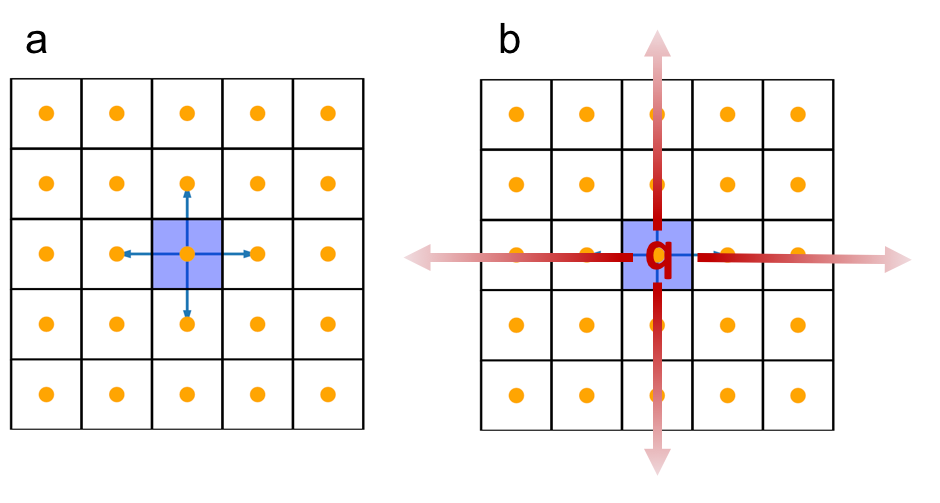
\includegraphics[width=0.75\textwidth]{figures/ase_defects.png}
    \caption{A charge-neutral defect interacting with periodic images of itself across periodic boundary conditions (a) and the longer-ranged Coulombic interactions of charged defects (b). Figure taken from reference \citenum{ase_defects} and adapted. ** MAKE OWN? - especially for benchmark write up and add charge to defect in (b)?**}
  \label{defect_PBCs}
\end{figure}

The supercell method is a common approach to simulate defects in the dilute limit and is the method that is utilised in section \ref{sulfosalt_defects}. This approach involves repeating the primitive unit cell a finite number of times in 3D and then embedding the defect within this larger unit cell so that the defect will be separated from its periodic image by a greater distance. If this distance is sufficiently large, the properties of an isolated defect can be represented by this model \cite{freysoldt_rev}.

\subsubsection{Charge neutral point defects}
** Ref Zhang and Northup (1991) for formation E eqn's? - double check! **\\

The formation energy, $\Delta H_{D,q=0}$, of charge neutral point defects in a supercell can be obtained by comparing the total energy calculated for the defective supercell to that of an equivalent perfect supercell of the host crystal and then considering the species added to or removed from the perfect supercell when the particular defect is formed. $\Delta H_{D,q=0}$ for a charge neutral defect is shown in Eq. \ref{defect_neutral} where $E_{D,q=0}$ is the total energy of the defective supercell, $E_{host}$ is the total energy of an equivalent supercell of the perfect, bulk host crystal, $n_i$ is the number of atoms of species i added to ($n_i > 0 $) or removed from ($n_i < 0$) the system when the defect is formed and $\mu_i$ is the chemical potential of species i. The chemical potential of a species i is the change in energy when one particle of type i is added to the system \cite{chem_pot}. In Eq. \ref{defect_neutral} $\mu_i$ allows us to describe the formation energy for defects in various growth conditions, such as rich or poor in particular species.
\begin{equation}\label{defect_neutral}
\Delta H_{D,q=0} = E_{D,q=0} - E_{host} - \sum_i n_i \mu_i
\end{equation}

\subsubsection{Charged point defects}
However, additional complexities arise when attempting to obtain the formation energy of a charged isolated point defect. Firstly, there is a strong and long-ranged Coulomb interaction between charged supercells in PBCs (indicated in Fig. \ref{defect_PBCs}b) and this converges slowly with increased supercell size.
Secondly, the charge of the defect system does not match that of the perfect bulk reference system. It is therefore necessary to introduce a chemical potential to account for the change in energy when electrons are added to or removed from the system when creating a defect in a given charge state.
Thirdly, electronic structure calculations with PBCs for a charged unit cell (effectively) include a neutralising homogeneous background charge to avoid infinite charge, which is not present in the calculation for the perfect equivalent supercell \cite{freysoldt_rev}. Consequently, the expression for the defect formation energy given in Eq. \ref{defect_neutral} for a charge neutral defect must be modified to that shown in Eq. \ref{defect_charged}.
\begin{equation}\label{defect_charged}
\Delta H_{D,q} = E_{D,q} - E_{host} - \sum_i n_i \mu_i + q[\epsilon_F + \epsilon_{\nu} + \Delta \nu_{0/b}] + E^q_{corr}
\end{equation}
Additional terms in Eq. \ref{defect_charged} compared to Eq. \ref{defect_neutral} are: q (the charge state of the defect), $\epsilon_F$ (position of the Fermi level in the band gap),  $q \epsilon_{\nu}$ (energy of bulk VBM) and $\Delta \nu_{0/b}$ (term used to align the electrostatic potential of the VBM for the bulk and defect supercells) and $E^q_{corr}$ (usually represents multiple post-DFT calculation corrections, one such correction is that for interactions between a charged defect and its periodic images, the `image-charge' correction but another is the `band filling' correction, both of which are outlined later). The latter term is to account for the introduction of the homogeneous background charge in electronic structure calculations of charged supercells, which is discussed further in the next section. The terms in Eq. \ref{defect_charged} are explained pictorially in Fig. \ref{pylada_eq}.
\begin{figure}[h!]
  \centering
    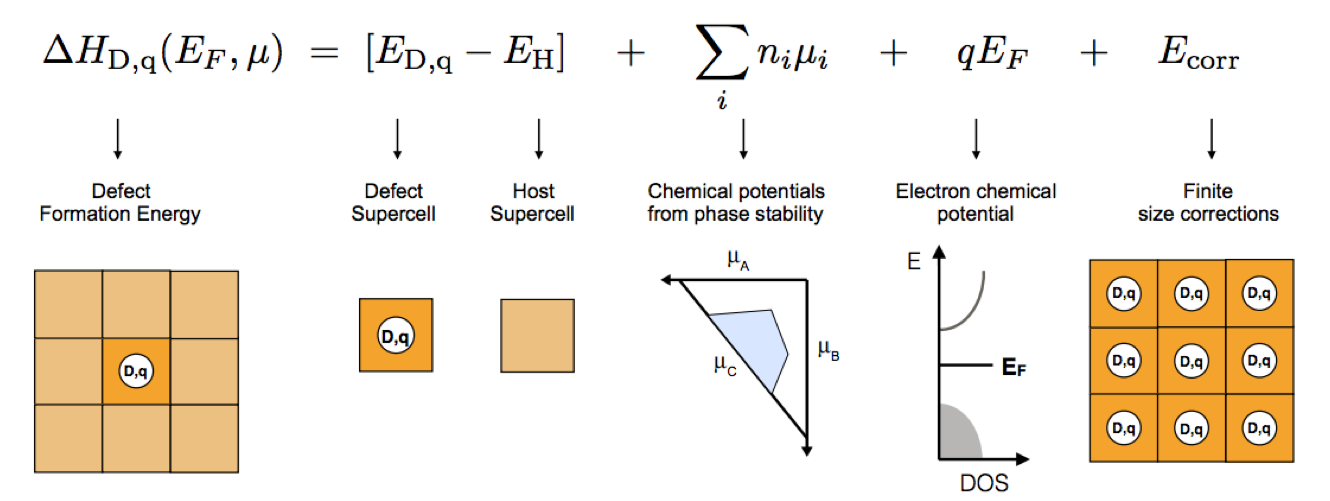
\includegraphics[width=0.95\textwidth]{figures/pylada_eq.png}
    \caption{Visual descriptions of terms in the equation for the formation energy of charged defects. Figure taken from Ref. \citenum{pylada}.}
  \label{pylada_eq}
\end{figure}

In theory, it is possible to continually increase the supercell dimensions to allow estimations of the magnitude and decay behavior of the different effects to be obtained and, from this, extrapolate to the formation energy of a defect in the limit of an infinitely large supercell.
However, due to computational limitations, it is usually not feasible to perform calculations with sufficiently large supercells to remove all spurious defect-defect interactions, especially for the long-ranged Coulombic interaction of charged defects, as depicted in Fig. \ref{defect_PBCs}b.
Furthermore, the band gap error in standard-DFT can cause large errors in the calculated properties of defects \cite{Lany_defects}. For this reason, methods beyond standard-DFT such as hybrid-DFT (outlined in section \ref{elec_struc}) may be used to more accurately predict the electronic structure. However, the computational expense for such methods is increased further, hence performing calculations for larger supercells becomes a less feasible endeavor.
Methods such as the supercell approach are used to minimise the impact of defect-defect interactions on calculated properties and various schemes have been developed to correct a posteriori for any remaining effects whenever possible \cite{freysoldt_rev}. Some such schemes are outlined in the next section and a study conducted to compare defect formation energies obtained from different schemes implemented with different electronic structure codes is presented in section \ref{defect_benchmark}.

\subsection{Finite-size corrections to defect supercells}

\subsubsection{Potential alignment}
The formation energy of a charged defect depends on the Fermi level, as shown in Eq. \ref{defect_charged} and this is referenced to the VBM of the host as the defect formation energy is related to the energy required to add or remove electrons to or from the VBM of the host from or to a Fermi reservoir \cite{Alex_defects}.
As already mentioned, when a charged defect is embedded in a supercell in a periodic electronic structure calculation, there will also be a compensating background charge. Otherwise, the Ewald summation performed in the electronic structure code to calculate the electrostatic energy of the system diverges, i.e. the system has an infinite charge. The effect of including a compensating homogeneous background charge is equivalent to setting the average electrostatic potential to zero \cite{freysoldt_rev}. 
In practise this corresponds to removing a constant in the Fourier transform of the electrostatic potential and the consequence of this treatment is that the eigenvalues are defined only up to an undetermined constant \cite{kumagai_oba, kumagai_oba_9}.
Although referred to as adding a `homogeneous background charge' in the electronic structure calculation, the charge compensation occurs only in the potential. A background charge density is usually not explicitly introduced into the calculation. If instead a compensating charge density was introduced, the resulting overall charge-neutral system should have a well-defined total energy and not depend on the undetermined constant \cite{Lany_defects, Lany_defects_2008}.
This correction step of course will only be applied to the charged defect supercell in the electronic structure calculations, and not to the perfect host. It is therefore necessary to align the average electrostatic potential in the perfect host supercell to that of the charged defect supercell before computing the defect formation energy through comparisons of the two systems with Eq. \ref{defect_charged}.
 
 Different approaches for potential alignment have been proposed in the literature, including using averages over the electrostatic potential in a small sphere around an atom, as in the Lany-Zunger (LZ) scheme \cite{Lany_defects}, and through the average over transversal planes in the `alignment-like' term in the Freysoldt, Neugebauer, Van de Walle (FNV) scheme \cite{FNV, kumagai_oba}. In both cases, the treatment involves comparing the averaged potential in the bulk-like region of the defect supercell (i.e far from the defect site) to that of a perfect bulk system. Although the electronic structure far from the defect may be similar in the defect supercell and the perfect reference, the average electrostatic potential in equivalent regions of each system could differ by a constant, due to the treatment described above \cite{komsa}. This constant can then be used in Eq. \ref{defect_charged} to align the VBM of the the perfect reference to the defect system.
 However, there is some debate in the literature as to whether this potential alignment step is required as a separate correction step, or, if it is in fact accounted for in the image-charge correction \cite{kumagai_oba}, which is outlined next.



\subsubsection{Image-charge correction}
Image-charge corrections are applied a posteriori to calculated total energies of charged defect supercells to account for the spurious interactions of defects with their periodic images, which were depicted in Fig. \ref{defect_PBCs}, and also with the neutralising `homogeneous background charge'. 
%and a number of schemes have been developed to correct for this error (Kumagai/ Oba paper ref 7, 11-18)
%This step involves considering three systems, firstly there is the perfect host system (the supercell without the periodically repeated charged defect). This is the reference system used to compare to the next two systems to determine the energy of the defect in each case. Secondly, there is a system with a periodic array of localised charged defects of charge q with a neutralising background charge.
%, where the defect interacts both with its periodic image and the neutralising background charge. 
%of $-\frac{q}{\Omega}$ (where $\Omega$ is the volume of the supercell unit).
This step involves considering two systems. Firstly there is a system with a periodic array of localised charged defects of charge q with a neutralising background charge.
This corresponds to the bare result of the electronic structure calculation for the charged defect supercell which needs to have energy corrections applied to it due to spurious interactions caused by the PBCs. Secondly, a system is considered that is just an isolated charge q in a dielectric medium (used to represent the host crystal), where more sophisticated models also take into account the anisotropy of the dielectric response of the host material \cite{kumagai_oba}.
Different models have been developed to quantify the effects of image-charge interactions in electronic structure calculations for the defect supercell through comparisons of the defect formation energy in these two systems.

%The simplest model for the latter system of an isolated point defect in a dielectric medium is to subtract point-charge energies \cite{kumagai_oba}
The magnitude of interactions between the charged defect with its periodic images can be estimated from the screened Madelung-like energy of an array of point charges \cite{LeslieGillan}.
The interaction decays asymptotically as $\frac{q^2\alpha}{2 \epsilon L}$ where L is a representative supercell dimension, $\epsilon$ is the dielectric constant of the host material (when an isotropic approximation is used) or the dielectric tensor otherwise \cite{kumagai_oba} and $\alpha$ is the Madelung constant which depends on the supercell geometry and can be calculated for any Bravais lattice through the use of the Ewald method \cite{Ewald, komsa}.
Makov and Payne (MP) derived an extension of the Madelung lattice sum for a more extended (but still localised charge) distribution \cite{MP}, shown in Eq \ref{MP} \cite{komsa}.
MP proved that for isolated ions the quadrupole moment of the charge distribution gives rise to a further term scaling as $L^{−3}$ \cite{MP, freysoldt_rev}.
\begin{equation}\label{MP}
E^{MP}_{corr} = E_{MP1} + E_{MP2} = \frac{q^2\alpha}{2 \epsilon L} - \frac{2 \pi q Q}{3 \epsilon L^3}
\end{equation}
where
\begin{equation}\label{MP_Q}
Q = \int r^2 \rho_c(\mathbf{r}) d\mathbf{r}
\end{equation}
is the second radial moment of the extended charge density.

However, Q in Eq. \ref{MP} cannot be calculated directly for defects in crystalline materials \cite{kumagai_oba, komsa, Lany_defects_2008}. Therefore in practise when using the MP scheme $E^{MP}_{corr}$ is usually not calculated but is estimated by fitting Eq. \ref{MP} to the formation energies calculated for defects with increased supercell size and then extrapolating to the infinite supercell limit. As already discussed, at high levels of theory such large systems may be computationally unfeasible. Furthermore, it has been shown that Eq \ref{MP} does not always give a good fit to calculated defect formation energies, creating doubt regarding the predictive power of this scheme \cite{FNV}. A number of alternative schemes have been proposed that do not require the use of increasing supercell sizes \cite{MP, LeslieGillan, PeterSchultz, Lany_defects, FNV, kumagai_oba}, here the LZ \cite{Lany_defects} and FNV \cite{FNV} schemes will be outlined as these methods will be used to calculate defect formation energies and the results will be compared in section \ref{defect_benchmark}.

\begin{figure}[h!]
  \centering
    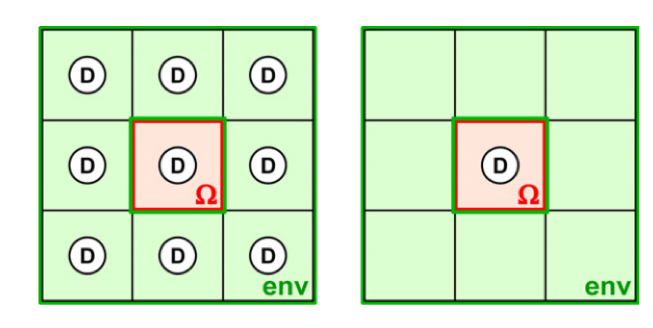
\includegraphics[width=0.8\textwidth]{figures/LZ_ic.png}
    \caption{A defect supercell of volume $\Omega$ in an environment (env) of periodic images of the defect (left) and in an environment of surrounding perfect, unperturbed supercells of the host lattice (right). Figure taken from Ref. \citenum{Lany_defects}.}
  \label{LZ_ic}
\end{figure}

The MP scheme \cite{MP} discussed above was developed for molecular systems and when calculating Q in Eq. \ref{MP_Q} the part of the defect charge density, $\rho_c(\mathbf{r})$, due to the electronic screening from the host crystal is not included \cite{Lany_defects_2008, Lany_defects}. However, it has been shown that Q is dominated by this contribution in crystalline solids \cite{Lany_defects_2008}. The LZ scheme, as outlined in Ref. \citenum{Lany_defects}, was devised to resolve this situation when calculating the image-charge correction for charged defects in crystalline solids. Firstly, the LZ scheme initially also considers the quadrupole-quadrupole contribution (whereas the MP scheme considers point-charge to point-charge in the MP1 term and point-charge to quadrupole in the MP2 term). If $\rho_c(\mathbf{r})$ is expected to be dominated by the screening response of the host, then it is not confined to the supercell and interactions between extended densities should also be considered \cite{Lany_defects}.
The image-charge correction is determined in the LZ scheme by considering the difference between the electrostatic interaction energy of the supercell with an environment of
unperturbed host supercells minus the interaction energy of the supercell with an environment of identical defect supercells, as shown on the right and left hand sides of Fig. \ref{LZ_ic} respectively. This is expressed in Eq. \ref{LZ_Ecorr1} where $\rho_H^{tot}$ is the charge density in the unperturbed perfect host supercell, $\Delta \rho_D$ is the difference between the charge density in the defect supercell and the perfect host supercell and $\Delta \rho_p$ is point-charge-like contribution to the change in the charge density due to the ionic substitution involved in the formation of the crystallographic defect.
\begin{equation}\label{LZ_Ecorr1}
\Delta E_i = - \int_{\Omega} dr^3 ( \rho_H^{tot}(\mathbf{r}) + \Delta \rho_p(\mathbf{r}) + \Delta \rho_D(\mathbf{r}) ) \int_{env} dr^{\prime 3} \frac{\Delta \rho_p(\mathbf{r^{\prime}}) + \Delta \rho_D(\mathbf{r^{\prime}})}{ | \mathbf{r} - \mathbf{r^{\prime}} | }
\end{equation}
Eq. \ref{LZ_Ecorr1} can be interpreted as Eq. \ref{LZ_Ecorr2} by making some assumptions. Firstly, that the interaction energy of $\rho_H^{tot}$ with the total defect-induced charge density in the image supercells ($\Delta \rho_p(\mathbf{r^{\prime}}) + \Delta \rho_D(\mathbf{r^{\prime}})$) can be neglected (provided that the defect supercell is sufficiently large). Secondly, that the second integral in Eq. \ref{LZ_Ecorr1} can be interpreted as the screened potential, $V_{scr}^{env}(\mathbf{r})$, by assuming that $\Delta \rho_D(\mathbf{r})$ essentially reflects the screening response of the host crystal to the defect.
\begin{equation}\label{LZ_Ecorr2}
\Delta E_i = - \int_{\Omega} dr^3 ( \Delta \rho_p(\mathbf{r}) + \Delta \rho_D(\mathbf{r}) ) V_{scr}^{env}(\mathbf{r})
\end{equation}
The interaction energy of $ V_{scr}^{env}(\mathbf{r})$ with $\Delta \rho_p(\mathbf{r})$ corresponds to the MP1 term in the MP scheme and the interaction with $\Delta \rho_D(\mathbf{r}) $ corresponds to the MP2 term in the MP scheme when the screening response of the host lattice is included in $\Delta \rho_D(\mathbf{r})$.

The expression in Eq. \ref{LZ_Ecorr2} can then be simplified by exploiting the observation that the delocalised part of the defect density, $\Delta \rho_D(\mathbf{r})$, is dominated by the screening response of the host. The consequence is that Q in Eq. \ref{MP_Q} is proportional to $q L^2$. The second term in Eq. \ref{MP} is then proportional to $\frac{q^2}{L}$ instead of $\frac{q}{L^3}$. By also assuming that the electronic charge accumulation at a defect is drawn homogeneously from the entire supercell \cite{Lany_defects_2008}, the image-charge correction can be expressed as the first-order correction to the MP1 term shown in Eq. \ref{LZ_Ecorr}, which depends only on the dielectric constant of the host, $\epsilon$, and the shape factor $c_{sh}$, which depends only on the shape of the host supercell (FCC, BCC, etc.) and has been calculated for several types of supercell shape in Ref. \citenum{Lany_defects}.
\begin{equation}\label{LZ_Ecorr}
E_{corr}^{LZ} = [1 + c_{sh} (1 - \epsilon^{-1}) ] E_{MP1}
\end{equation}
In the LZ scheme the potential alignment correction is performed independently of the image-charge correction.

The FNV scheme, as outlined in Ref. \citenum{FNV}, differs from the LZ scheme in that it does not depend upon the shape of the supercell and does not involve a separate potential alignment step, this is instead incorporated in the image-charge correction with the `alignment-like' term. The FNV scheme considers two contributions to the correction term: the interaction energy of a defect with periodic images ($E^{inter}$) and the interaction energy of the background charge with the defect inside the reference supercell ($E^{intra}$).
These contributions are combined to give the correction term shown in Eq. \ref{FNV_corr}.
\begin{equation}\label{FNV_corr}
E_{corr}^{FNV} = E^{inter} + E^{intra} = E^{latt}_q - q\Delta_{q/0}
\end{equation}
where
\begin{equation}\label{E_latt}
E^{latt}_q = \int_{\Omega} d^3 \mathbf{r} \Big[ \frac{1}{2} [q_d(\mathbf{r}) + n ] [\tilde{V}^{lr}_q(\mathbf{r}) - V^{lr}_q(\mathbf{r}) ] + nV^{lr}_q(\mathbf{r}) \Big]
\end{equation}
and
\begin{equation}\label{alignmentlike}
\Delta_{q/0} = \frac{1}{\Omega} \int_{\Omega} d^3 \mathbf{r} V^{sr}_{q/0}(\mathbf{r})
\end{equation}
$q_d(\mathbf{r})$ is the unscreened charge density of the defect which is assumed to be contained entirely within the supercell. $\Omega$ is the volume of the supercell. $V_{q}$ is the electrostatic potential for defect with charge q, $q/0$ corresponds to the electrostatic potential for the charged defect with charge q minus that for a neutral defect (where q=0). Tildes are used to denotes values for the system from the periodic electronic structure calculation. The $lr$ and $sr$ superscripts correspond to the long range and short range components of the potential, where the lr will be dominated by the macroscopically screened Coulomb potential and sr accounts for variations in the microscopic screening.
%FNV eq6
%FNV eq7

A value for Eq. \ref{E_latt} can be obtained by taking a suitable approximation for the defect charge density in the supercell, $q_d$, such as a point charge or a Gaussian and then performing an Ewald summation.
Eq. \ref{alignmentlike} is the `alignment-like' term in the FNV scheme and $V^{sr}_{q/0}$ is given by Eq. \ref{alignmentlike2}. In this expression $\tilde{V}_{q/0}(\mathbf{r})$ is obtained directly from the electronic structure calculation and the alignment constant, C, is determined by plotting average potentials in the xy plane as a function of z and taking the difference between plots of $\tilde{V}_{q/0}$ and $\tilde{V}^{lr}_{q}$ where the two plots plateau.
\begin{equation}\label{alignmentlike2}
V^{sr}_{q/0} =  \tilde{V}_{q/0}(\mathbf{r}) - \tilde{V}^{lr}_{q}(\mathbf{r}) - C 
\end{equation}


\subsubsection{Band filling correction}

%Key sections of \cite{Lany_defects_2008}:
%\begin{itemize}
%\item Section II, D. “Postprocessor” corrections to supercell energies, 3. Band-filling correction (SSE)
%\item Section IV, B. Finite-size effects due to host and impurity band dispersion, 1. Total-energy contributions due to band filling
%\item Summary last para
%\item + ref 5 \cite{CIS_defects}
%\end{itemize}

The above correction methodologies require that the charge of the defect is localised within the supercell unit. However, this is not always the case. Large finite-size effects that converge slowly with increased supercell size have been observed for some defects, even in charge neutral states. This has been attributed to ‘band filling’ effects from high defect concentrations in typical finite-size supercells \cite{Lany_defects_2008, CIS_defects, pylada}. This effect is typically more pronounced for shallower defects. Shallower defects typically have more delocalised wavefunctions associated with them, therefore increasing the likelihood of the defect wavefunction extending beyond the boundary of the supercell unit. Consequently, it is possible for even neutral defects to interact with defect-images in adjacent supercells. 

Defect-defect interaction means that the defect-induced energy level may interact with that of its image to form a defect band with a dispersion in the band energies that would not be present for a distinct, localised defect level that would be expected for a defect in the dilute limit. In the case of a donor defect, the electrons may now occupy defect-induced energy levels in the defect band at higher energies than would be possible in the dilute limit due to the dispersion of the defect band. This could then also lead to spurious hybridisation of defect bands with the host electron states, and the donor electrons can partly populate the host conduction bands, giving rise to band filling effects (Moss-Burstein shift) \cite{Lany_defects_2008}.

A correction step for such effects has been proposed \cite{CIS_defects, Lany_defects_2008, Lany_defects} and is to be applied after performing the potential alignment step in the LZ scheme outlined above.
To correct the total energy of the finite supercell due to the band-filling effects, the higher energy populations are subtracted \cite{CIS_defects}.
For a given \textit{k}-point set (weighted sum, $w_k$) and band occupations, $\eta_{n,k}$, the correction for a shallow donor is obtained from Eq. \ref{band_filling_donor} and for a shallow acceptor from Eq. \ref{band_filling_acceptor}, where $e_{n,k}$ are the band energies in the defect calculation, $\tilde{e}_c$ and $\tilde{e}_v$ are the CBM and VBM energies respectively of the pure host after performing the potential alignment step within the LZ scheme \cite{pylada}.
\begin{equation}\label{band_filling_donor}
E_{BF} = - \sum_{n,k} w_k \eta_{n,k} [e_{n,k} - \tilde{e}_c]
\end{equation}
\begin{equation}\label{band_filling_acceptor}
E_{BF} = - \sum_{n,k} w_k (1 - \eta_{n,k}) [e_{n,k} - \tilde{e}_v]
\end{equation}
However, if the intention is to simulate defects in highly doped semiconductors, the corrections in Eq. \ref{band_filling_donor} and \ref{band_filling_acceptor} should be zero or at least smaller since the formation of defect bands with band dispersion and heavy band filling should be present in a system where defect-defect interactions are a correct physical representation \cite{CIS_defects}.


\section{Modeling imperfect solids: Extended antisite defects}\label{MC}
In this section defects and disorder is considered on much larger scales than is computationally feasible from electronic structure calculations.
Here, the fundamentals of utilising the Monte Carlo method to describe thermodynamic substitutional disorder are outlined. This is equivalent to investigating interacting extended antisite defects at higher defect concentrations than would be considered as the `dilute', non-interacting limit. This method is applied to study Cu-Zn disorder in {\CZTS} in \autoref{chap:CZTS}.
%**Introduce general method (see transfer report + cross-ref extra textbooks** \cite{MC} = Newman, \cite{MC_Landau} and \cite{MC3} (Topic in current physics)

\subsection{The Monte Carlo method for equilibrium thermodynamics}
The Monte Carlo (MC) method allows for the simulation of systems with many degrees of freedom. Its name derives from its use of (pseudo-)random numbers to simulate statistical fluctuations in order to numerically generate probability distributions \cite{MC3}.
The MC method in statistical physics is a special case of the more general MC method.
Starting from a model hamiltonian, the method can be used to calculate thermodynamic information about a system of N interacting ions represented on a 3D lattice by using classical statistics, considering only two-body forces and assuming that the potential field of an ion is spherically symmetric. If we know the positions of the N interacting ions on the lattice then the potential energy of the system can be calculated using equation \ref{pot_E}, where V is the Coulombic potential between two ions and $d_{ij}$ is the minimum distance between ions i and j \cite{Metropolis}.
\begin{equation}\label{pot_E}
E = \frac{1}{2} \sum_{i=1}^N \sum_{j=1}^N V d_{ij}
\end{equation}
To calculate the properties of the system, the canonical ensemble is used where the temperature, number of ions and volume are all constant. In this ensemble, the equilibrium value for any quantity of interest, B, is given by equation \ref{av}, where $E_\alpha$ is the energy of the system when in state $\alpha$ and $p_\alpha$ is the probability of the system being in state $\alpha$.
\begin{equation}\label{av}
<B> = \frac{ \sum_\alpha e^{-\frac{E_\alpha}{k_bT}} B_\alpha}{ \sum_\alpha e^{-\frac{E_\alpha}{k_bT}}} = \frac{ \sum_\alpha e^{-\frac{E_\alpha}{k_bT}} B_\alpha}{Z} = \sum_\alpha B_\alpha p_\alpha
\end{equation}
\begin{equation}\label{prob}
p_\alpha = \frac{  e^{-\frac{E_\alpha}{k_bT}} }{ \sum_{\alpha} e^{-\frac{E_\alpha}{k_bT}}} =\frac{  e^{-\frac{E_\alpha}{k_bT}} }{Z}
\end{equation}
$Z$ in equation \ref{av} is called the partition function. For most systems calculating the value of the partition function requires the summation over a large number of states. When applying the Monte Carlo method to a system of particles, the summation over discrete states for $Z$ is replaced by a set of integrals. This is shown in equation \ref{MC_av} where $U(\mathbf{r}^N)$ is the potential energy of the system which depends upon the position, \textbf{r}, of the N interacting ions in the system and $Z_{NVT}$ is the configurational integral \cite{Lesar3}.
%\begin{equation}\label{MC_prob}
%p(\mathbf{r}^N) = \frac{  e^{-\frac{U(\mathbf{r}^N)}{k_bT}} }{\int %e^{-\frac{U(\mathbf{r}^N)}{k_bT}} d\mathbf{r}^N}  = \frac{  e^{-\frac{U(\mathbf{r}^N)}%{k_bT}}}{Z_{NVT}} 
%\end{equation}
\begin{equation}\label{MC_av}
<U> = \frac{ \int e^{-\frac{U(\mathbf{r}^N)}{k_bT}} U(\mathbf{r}^N) d\mathbf{r}^N}{\int e^{-\frac{U(\mathbf{r}^N)}{k_bT}} d\mathbf{r}^N}  = \frac{  \int e^{-\frac{U(\mathbf{r}^N)}{k_bT}} U(\mathbf{r}^N) d\mathbf{r}^N}{Z_{NVT}} 
\end{equation}
The configurational integral is over the three coordinates of each ion, as shown in equation \ref{dr}. There are therefore 3N coordinates that define all possible configurations of the system.
\begin{equation}d \mathbf{r}^N = dx_1 dy_1 dz_1 dx_2 dy_2 dz_2... dx_N dy_N dz_N\end{equation}\label{dr}
For a system containing several hundred ions this would be a several-hundred dimensional integral over the configuration space, which would be impractical to carry out by the usual numerical methods. The Monte Carlo method for many-dimensional integrals is used for this purpose \cite{Metropolis}. It is conceptually easiest to think about this method for a one-dimensional integral. This method involves sampling a large number of random points within a region defined by the limits of the integral. The integrated function is then the fraction of points that fall below the curve of the function multiplied by the area of the sampled region. The value obtained becomes a better approximation to the actual value of the integral as the number of random numbers, called Monte Carlo steps (MCS), used to sample the integration region increases. \cite{Lesar3}.


\subsubsection{Monte Carlo simulation with the Metropolis Algorithm }
The Standard MC method for our system would involve placing each of the N ions at random positions in the lattice to define a random point in the 3N-dimensional configuration space. The energy of the system would then be calculated using equation \ref{pot_E} and the configuration would then be weighted using $e^{-\frac{U(\mathbf{r}^N)}{k_bT}}$ when obtaining the equilibrium value of U. However, many configurations are very improbable so performing this calculation for every possible configuration would be inefficient and unnecessary to sufficiently evaluate the ensemble. The custom MC code in this study makes use of the Metropolis modified MC scheme \cite{Metropolis}. In this implementation of the MC method, instead of choosing configurations randomly and then weighting them, the Metropolis algorithm considers the relative probability of a system being in a new configuration, $\beta$, to that of being in the current configuration, $\alpha$. This is shown in equation \ref{relative_prob}, where $E_\alpha$ is the energy of state $\alpha$ and $E_\beta$ is the energy of state $\beta$.
\begin{equation}\label{relative_prob}
\frac{p_\beta}{p_\alpha} = \frac{  e^{-\frac{E_\alpha}{k_bT}} }{Z} \frac{Z}{  e^{-\frac{E_\alpha}{k_bT}} } = e^{- \frac{E_\beta - E_\alpha}{k_BT}}
\end{equation}
The relative probabilities of the two states are completely determined by the energy 
difference, such that if:
\begin{equation}\label{met}
\Delta E = E_{\beta} - E_{\alpha} \leq 0    \quad  then  \quad   \frac{p_{\beta}}{p_{\alpha}} \geq 1 
\end{equation}
and if
\begin{equation}\label{met2}
\Delta E = E_{\beta} - E_{\alpha} > 0   \quad   then   \quad   \frac{p_{\beta}}{p_{\alpha}} < 1
\end{equation}

The Metropolis algorithm creates a list of configurations through configuration space that has the correct probability distribution. This list is called a trajectory through configuration space. The approach involves making a trial move of the system to a new configuration. In the case of the study presented in section \ref{CZTS_MC} this would be a substitution between a Cu and a Zn ion in an on-lattice model of {\CZTS}. It is then decided if this new configuration should be added to the trajectory or not based on the probability of the new configuration relative to the current configuration. If the relative probability is  $\geq$ 1, as shown in equation \ref{met}, then the move is accepted and added to the trajectory. However, if the relative probability is $<$ 1 then the move will only be accepted if $e^{-\frac{\Delta E}{k_BT}} \ge$ a random number generated between 0 and 1 \cite{Lesar3}. Provided a sufficiently large number of trial moves have been made, from this procedure it is possible to obtain equilibrium disordered configurations for the ions in {\CZTS} at various simulation temperatures. The model developed for {\CZTS} is discussed further in the section \ref{Eris}.


 








\chapter{Performance bottlenecks of {\CZTS} solar cells}\label{chap:CZTS}
\section{Motivations and challenges for {\CZTS} solar cells}
Thin-film PV is a desirable contender for terawatt-scale renewable energy generation. Kesterite-structured {\CZTS} stands out for its potential for large-scale deployment due to the abundance and non-toxicity of its elemental components, as well as sunlight-matched direct band gap of 1.5 eV \cite{CZTS_rev}. In the following letter we outline some of the main bottlenecks for the advancement of this solar cell technology.

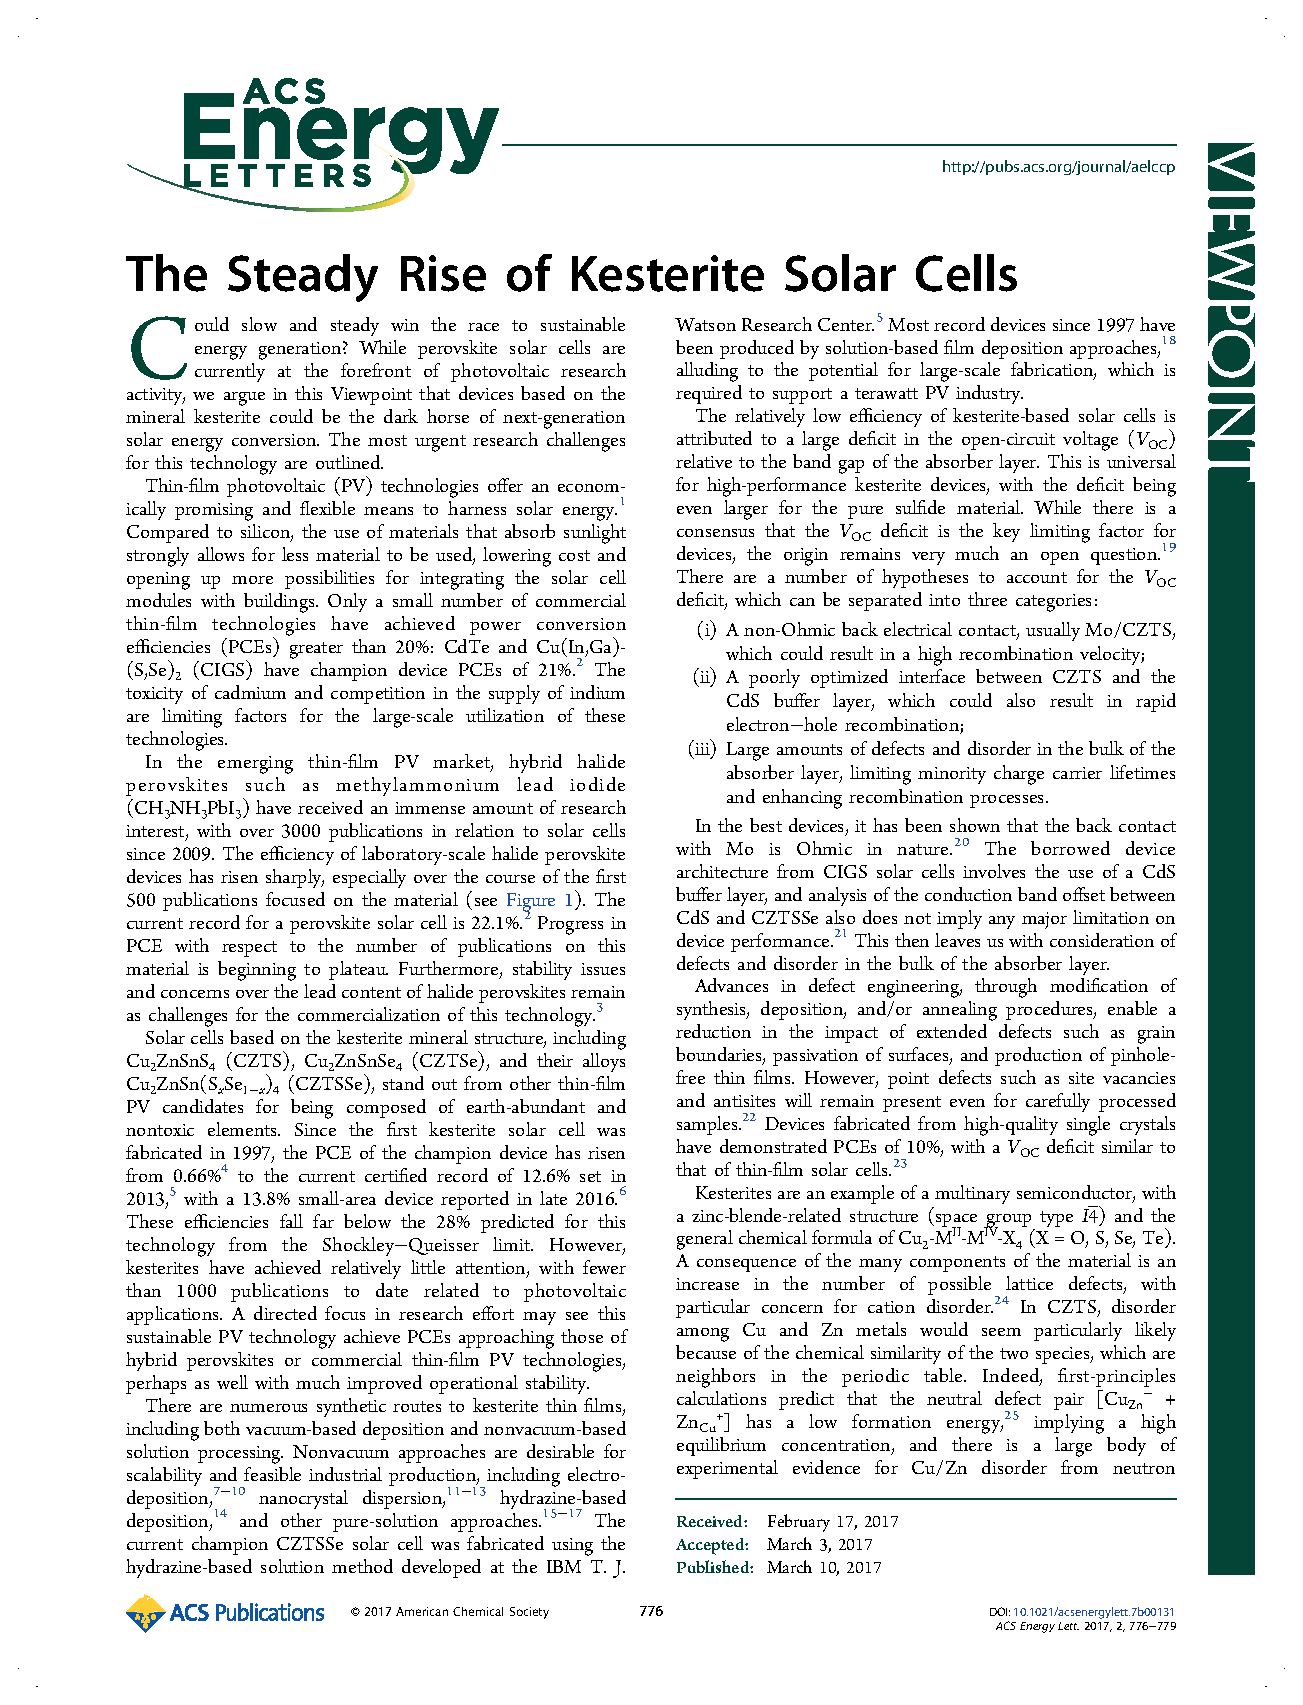
\includepdf[pages={1-},scale=1.0]{papers/CZTS_lett.pdf}


\section{Defects beyond the dilute limit in {\CZTS}}\label{CZTS_beyond_dilute}
Electronic structure calculations for the formation energies of point defects and point defect pairs in the dilute limit have already been calculated for {\CZTS}, where the [$Cu_{Zn}^- + Zn_{Cu}^+$] defect pair was found to have a particularly low formation energy \cite{defects_Chen}.
The calculations performed in Ref. \citenum{defects_Chen} were performed using the GGA functional with a rigid shift applied to the defect levels to account for the band gap error at this level of theory \cite{Lany_defects}. In Ref. \citenum{defects_Chen} one defect calculation was performed using a hybrid functional where it was found that the formation energy of the test defect differed by 0.1 eV. We therefore repeated the calculation of the formation energy for the defect pair of interest for our study.

For our calculation of the formation energy of the nearest-neighbour [$Cu_{Zn}^- + Zn_{Cu}^+$] defect pair, we make use of the Heyd-Scuseria-Ernzerhof (HSE06) hybrid-functional \cite{HSE} for the exchange-correlation functional as implemented in the Vienna Ab-initio Simulation Package (VASP) \cite{VASP}. This functional mixes 25\% of screened Hartree-Fock exchange to the Perdew-Burke-Ernzerhof (PBE) exchange functional \cite{PBE}. Projector augmented-wave potentials \cite{PAW} were used to describe the core electrons with an energy cut-off of 500 eV for the plane-wave basis set. Calculations were initially performed at the gamma point (a 1x1x1 \textit{k}-point mesh) until forces on the ions converged to within 0.01 eV/ $\AA$. 
A single geometry step was then performed with a 2x2x2 \textit{k}-point mesh centred on the gamma point as these parameters were found to be sufficient for the total energy to converge to within $<$2 meV  per atom with respect to increased plane-wave cut-off energy and for the external pressure to be $<$1 kbar. However, performing the full calculation with a 2x2x2 \textit{k}-point mesh was found to be too computationally expensive. 
%Data for the convergence test is given is table \ref{conv_test}. 
From our calculation, we predict a defect formation energy of 0.30 eV.

\begin{figure}[h!]
  \centering
    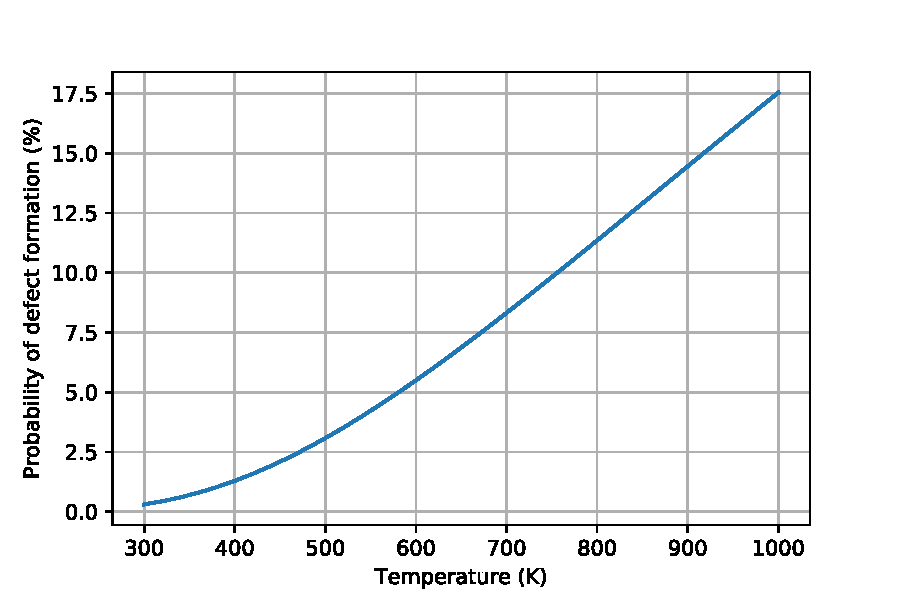
\includegraphics[width=0.9\textwidth]{figures/CZTS_Cu-Zn_defect_conc.pdf}
    \caption{Probability of nearest neighbour [$Cu_{Zn}^- + Zn_{Cu}^+$] defect formation as a function of temperature based on the equilibrium defect concentration from classical thermodynamics. The shaded region indicates typical annealing temperatures used in the synthesis of {\CZTS}.}
  \label{Cu-Zn_eqm_conc}
\end{figure}

When defect concentrations are less than 1\%, it is usually assumed that the system is in the dilute defect limit where defects can be considered to be non-interacting (**REF??? From Stoneham maybe? - check!**). Using statistical thermodynamics for point defects, an expression for the equilibrium concentration of point defects as a function of temperature can be obtained \cite{thermodynamics}. This is shown in equation \ref{defect_conc}, where N is the number of sites, $\Delta H$ is the defect formation energy, $k_B$ is the Boltzmann constant and T is the temperature of the system.
\begin{equation} \label{defect_conc}
n = Ne^{\frac{-\Delta H}{k_BT}}
\end{equation}
The probability of defect formation as a function of temperature is given by the exponential expression in equation \ref{defect_conc}. The defect formation energy from the DFT calculations were halved to take an average of the formation energy per defect during the formation of an antisite pair before being inserted into this expression. This is plotted against temperature in figure \ref{Cu-Zn_eqm_conc}. 
Even `low-temperature' synthesis procedures for {\CZTS} use annealing temperatures over 600K \cite{low_T_CZTS}. It can be seen from figure \ref{Cu-Zn_eqm_conc} that the probability of defect formation even at 600K is much higher than what would be considered as the `dilute limit' at 1\%.

Furthermore, there is experimental evidence of high concentrations of disorder \cite{Scragg, pot_fluc_4, neutron, Schorr}, indicating the likely formation of extended defect structures beyond point defects and pairs. To simulate such defect structures in {\CZTS} a bespoke Monte Carlo model was developed. This will be outlined in the next section and is applied in the study presented in section \ref{CZTS_MC}.


\section{Custom on-lattice Monte Carlo code for Cu-Zn disorder in {\CZTS}}\label{Eris}
The Monte Carlo model for Cu-Zn disorder is analogous to the Ising model of a ferromagnet, descriptions of which can be found in many textbooks such as references \citenum{MC} and \citenum{MC_Landau}. 
The Ising model uses interactions between spins, whereas our model considers the Coulombic interaction between the bare formal charges of ions in the lattice of {\CZTS}.
In the case of an Ising model, the trial moves in the Metropolis algorithm are spin flips, whereas in our model the trial moves are swaps between Cu and Zn ions. Typically, when performing simulations of an Ising model the calculated quantities of interest are the internal energy and average magnetization of the system as a function of temperature obtained by summing over the distribution of atomic spins. In the case of our system, the quantities of interest are the spatial arrangement of the Cu and Zn ions due to thermodynamic substitutions between the two species and the resulting distribution of electrostatic potential across the system for the implications this could have on band tailing. 

\begin{figure}[h!]
  \centering
    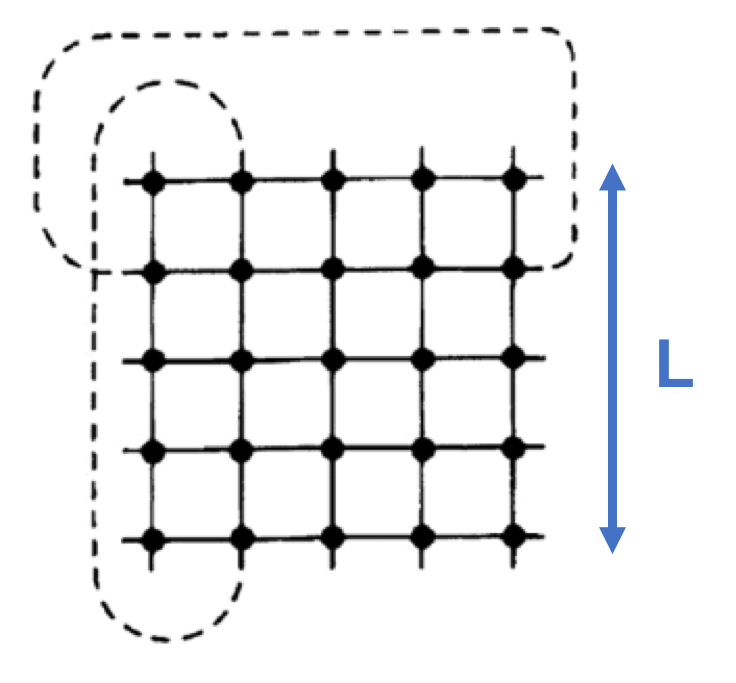
\includegraphics[width=0.4\textwidth]{figures/MC_PBCs.png}
    \caption{Typical periodic boundary conditions for the two-dimensional Ising model. Figure taken from \citenum{MC_Landau}.}
  \label{MC_PBCs}
\end{figure}

However, before we attempt to extract any information on thermodynamic disorder or the associated band tailing we would predict from such disorder, two important considerations for our model will be firstly to determine if the disordered configuration we obtain is in fact the equilibrated configuration at the given temperature and secondly if finite size effects are having an impact on the system properties we obtain from our simulations.
As simulations are performed for finite lattices, in order to simulate a bulk system the edges or `boundaries' of the system must be treated carefully. The boundaries can be effectively eliminated through the use of periodic boundary conditions (PBCs). In the case of an Ising model, this means that the first spin in a row interacts with the last spin in the row as if it were a nearest neighbour, and vice versa \cite{MC_Landau}. This principle is illustrated for a two-dimensional system in figure \ref{MC_PBCs}. Although this procedure effectively eliminates boundary effects, the system is still characterized by the finite lattice size, L, which limits the correlation length to $\frac{L}{2}$. Resultant properties of the simulated system may then differ from the bulk system. We therefore will need to perform simulations with increasing system size to look for any differences in the quantities of interest.

Determining if our system has reached equilibration at each temperature however may require a more complicated procedure. As the Monte Carlo method is stochastic, making use of sampling many times with random numbers to determine the minimum energy configuration of the system, the trajectory to reach this final configuration will by nature be random. Therefore, we can draw no conclusions about the properties of our system from evolved states until the final configuration at the particular temperature is reached. We therefore developed and tested methods to check for equilibration before we attempt to extract any thermodynamic properties of our system.

\begin{figure}[h!]
  \centering
    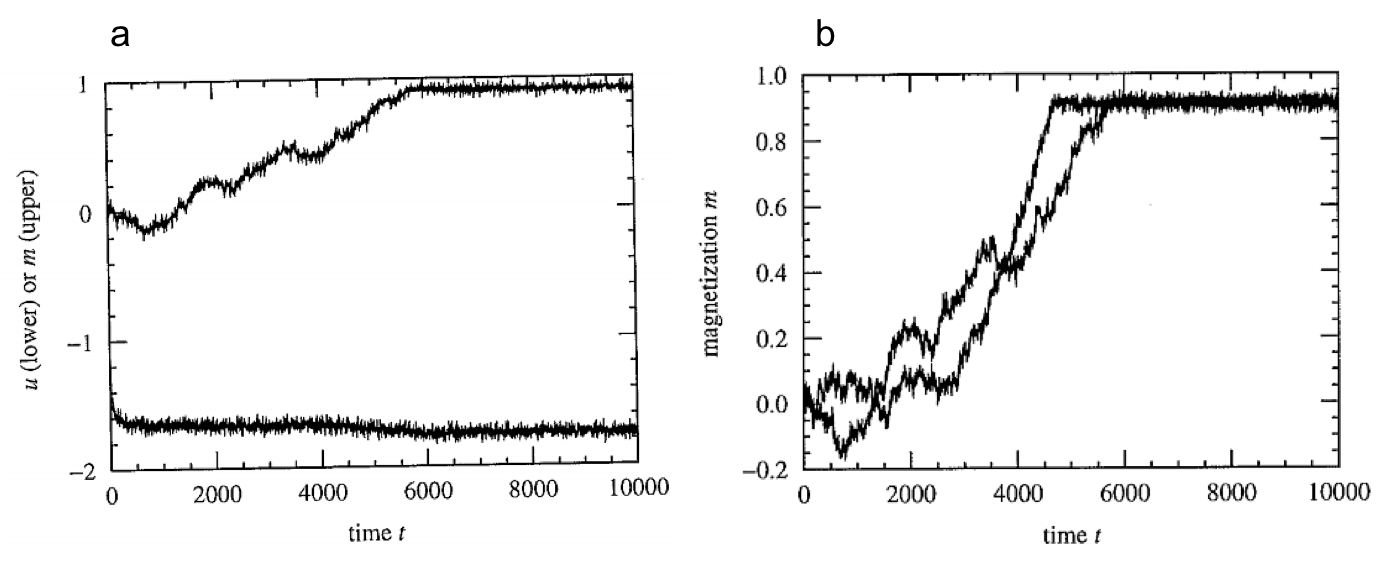
\includegraphics[width=0.9\textwidth]{figures/ising_equil.png}
    \caption{The magnetization (upper curve) and internal energy (lower curve) per site of a two-dimensional Ising model simulated using the Metropolis algorithm (a). Magnetization as a function of time for two different simulations (b). Time is measured in Monte Carlo steps per lattice site. Figures taken from \citenum{MC}.}
  \label{ising_equil}
\end{figure}

In the case of the Ising model when, for example, determining the average magnetization of a system at a given temperature, the simulation must be run for a suitably long time until the system has come to equilibrium at that temperature. This is referred to as the equilibration time. Once the system has equilibrated, the quantity of interest such as the magnetization must then be measured again over a suitably long time and averaged. 
To gauge if a system has reached equilibrium, in the case of the Ising model, it is common practice to run the simulation for a large number of Monte Carlo steps (MCS) (where one MCS corresponds to attempting a trial spin-flip at all sites in the system once) and looking for how the value of a quantity of interest, such as the average magnetization across the system, changes with increasing number of MCS as the simulation progresses. Equilibration is often considered as the point at which the value of a quantity of interest, which initially changes by a large amount, eventually converges to fluctuating about a steady average value. An example of this is shown in figure \ref{ising_equil}a. This is dependent upon the principle that a system in equilibrium spends the overwhelming majority of its time in a small subset of states in which its properties take a narrow range of values \cite{MC}. Provided the simulation has equilibrated, the final configuration for a given system at a given temperature should always be the same regardless of the initial configuration of the simulation, this point is illustrated in figure \ref{ising_equil}b.

Using this principle, one way to determine if our system has reached its equilibrium configuration could be to use perfectly ordered or disordered initial lattice configurations that. Both of these initial configurations, if the simulation is allowed to evolve over a suitable number of MCS, should eventually result in the same equilibrium system configuration. It would be difficult to distinguish differences in the atomic arrangement of one 3D lattice to another by eye, therefore comparisons of the radial distribution function (RDF) for each configuration as it evolves from either an ordered or disordered initial configuration can be made. 
Another method to check for equilibration is analogous to that shown in figure \ref{ising_equil}a for the Ising model. In the case of our system, it is the distribution of the electrostatic potential at Sn sites in the system that is of interest. As we fix Sn ions in our simulation we calculate the on-site electrostatic potential for Sn ions to study how the chemical environment of these species is altered by Cu-Zn disorder. One possible method to check for equilibration could be to look for a point after which the variance of the distribution of electrostatic potentials across the system has reached a steady value. Both of these methods were tested and are discussed in the study in section \ref{CZTS_MC}.

\begin{figure}[h!]
  \centering
    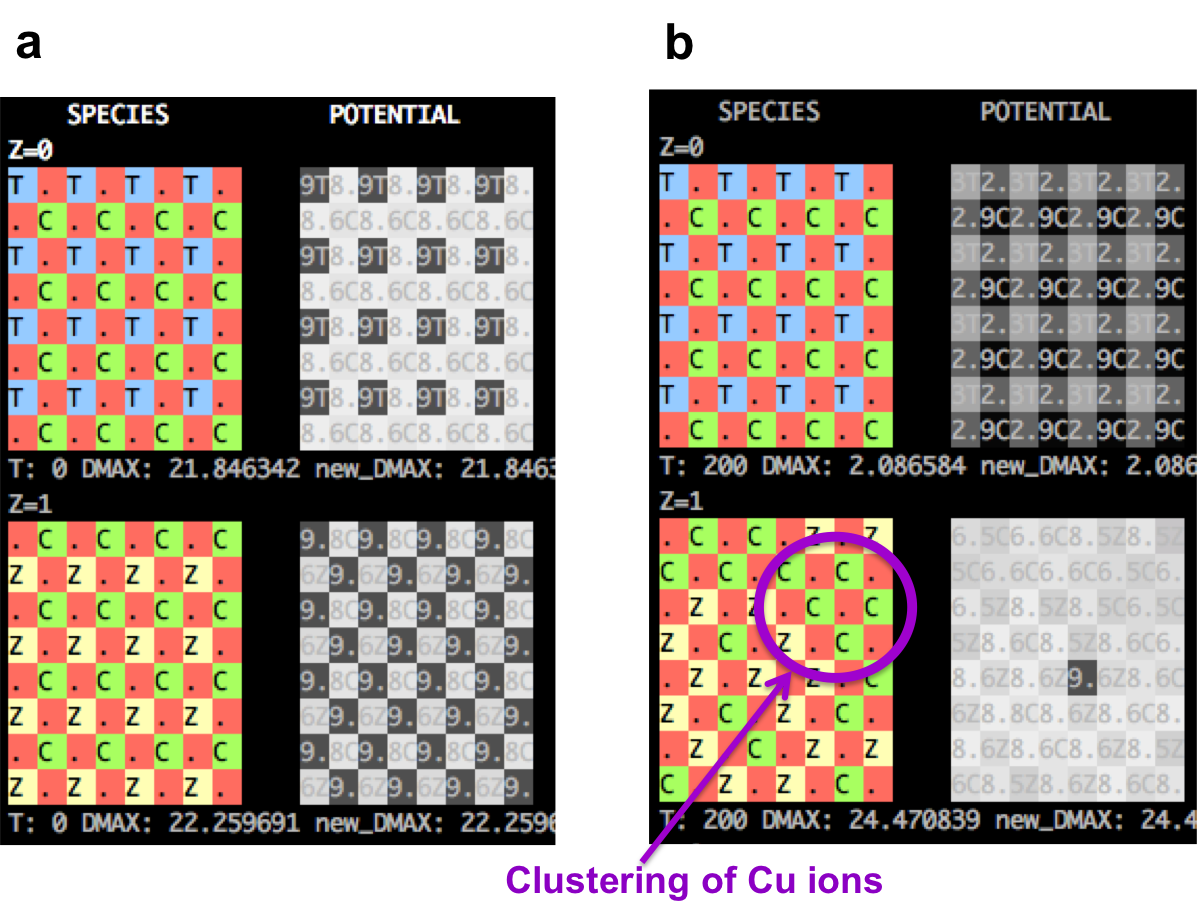
\includegraphics[width=0.9\textwidth]{figures/eris_spatial_disorder.png}
    \caption{Example outputs from Eris Monte Carlo simulations of Cu-Zn disorder from an initially ordered lattice showing the top two layers of the lattice when simulations are performed at temperatures T = 0K (a) and at T = 200K (b).}
  \label{eris_spatial_disorder}
\end{figure}

Monte Carlo simulations of thermodynamic substitutions between Cu and Zn ions will be allowed to evolve until the equilibrium configuration in terms of the arrangement of Cu and Zn atoms at the given temperature is reached. Fig. \ref{eris_spatial_disorder} shows an example output from our simulations, where the T = 0K spatial arrangement of cations in figure \ref{eris_spatial_disorder}a corresponds to the perfectly ordered system and the T= 200K configuration in figure \ref{eris_spatial_disorder}b shows spatial clustering of Cu and Zn ions as the system has been allowed to evolve at a finite temperature. The model is used to investigate and quantify thermodynamic Cu-Zn disorder in {\CZTS} in section \ref{CZTS_MC}. The electrostatic potential at each site in the lattice in disordered configurations can be calculated for later analysis of the distribution of electrostatic potential across the system due to Cu-Zn disorder. This will discussed further in section \ref{eris_future_work}. 




\section{Disorder processes during the Cu-Zn order-disorder transition in {\CZTS} from Monte Carlo simulations}\label{CZTS_MC}
For {\CZTS} a lot of attention in the literature has been paid to disorder amongst Cu and Zn cations with a large amount of experimental evidence for the presence of this disorder \cite{Schorr, CZTS_Xray, CZTS_TEM} and theoretical predictions for the low formation energy of the  $[Cu_{Zn}^{-} + Zn_{Cu}^{+}]$ \cite{defects_Chen}.
During the synthesis of {\CZTS}, temperatures above room temperature are used and it is possible for some of the thermal disorder associated with the system at higher temperatures to be `frozen in' to the material as it cools to room temperature.
Near resonant Raman spectroscopy has been used to examine thin films of CZTS prepared using different thermal treatments to determine if long post-annealing cooling times could produce films with a high level of order amongst Cu and Zn cations. However in this study, the authors postulate that achieving a very high level of order amongst Cu and Zn could require years \cite{Katharina}. This clearly wouldn't be a practical treatment for a PV device and so it would seem that the presence of a fairly large amount of disorder amongst Cu and Zn, and hence $Cu_{Zn}^{-}$ and $Zn_{Cu}^{+}$ antisites,  is inevitable in the material. In the following paper, we have developed a Monte Carlo model to gain atomistic insight into disorder in the cation sublattice. We simulate thermodynamic disorder in the Cu-Zn sublattice and quantify a baseline level of disorder to be expected for an optimally processed material with no kinetic limitations on cation ordering.\\

Introductory paragraph + Eris paper1 (methodology) + include paper SI? (or put in appendix?) + Add statement on personal contribution (or include this in previous section??) + link to Eris git repo and Zenodo doi for data?

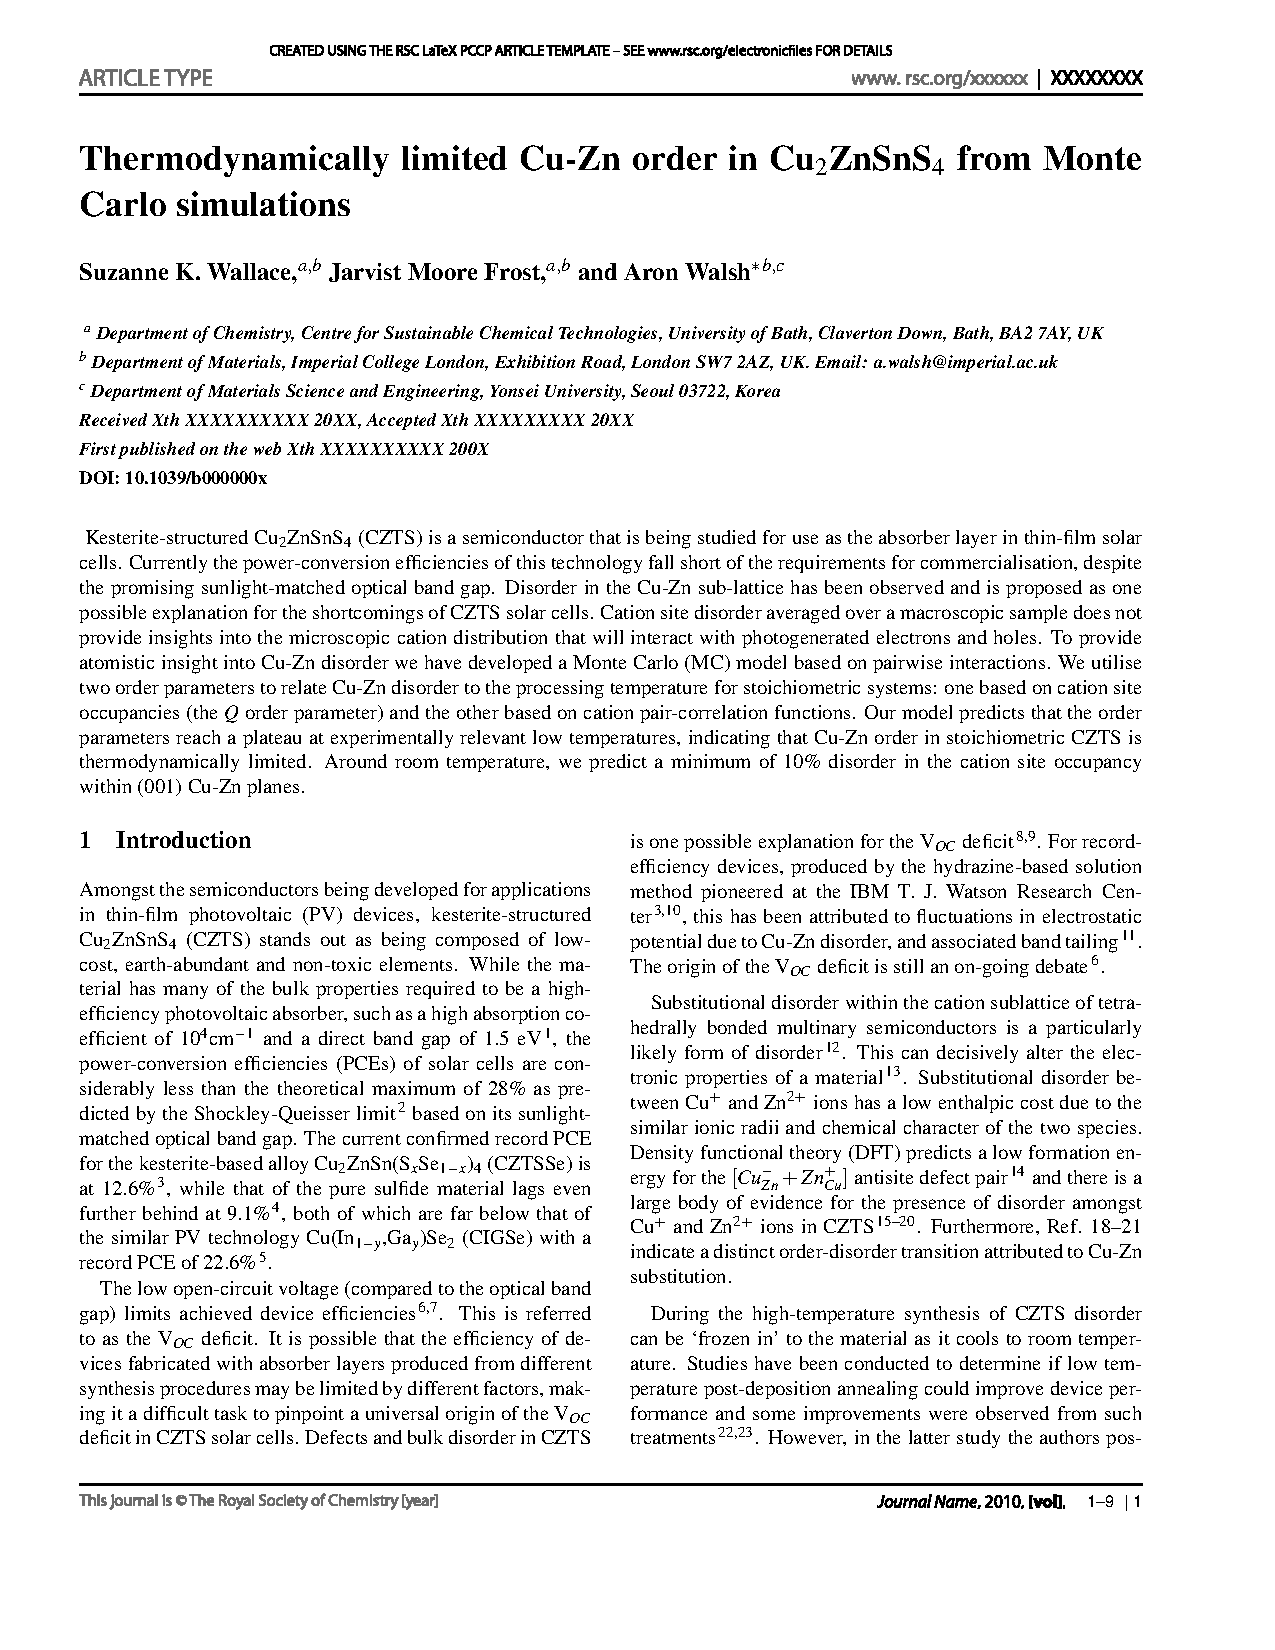
\includepdf[pages={1-},scale=1.0]{papers/ErisPaper1.pdf}
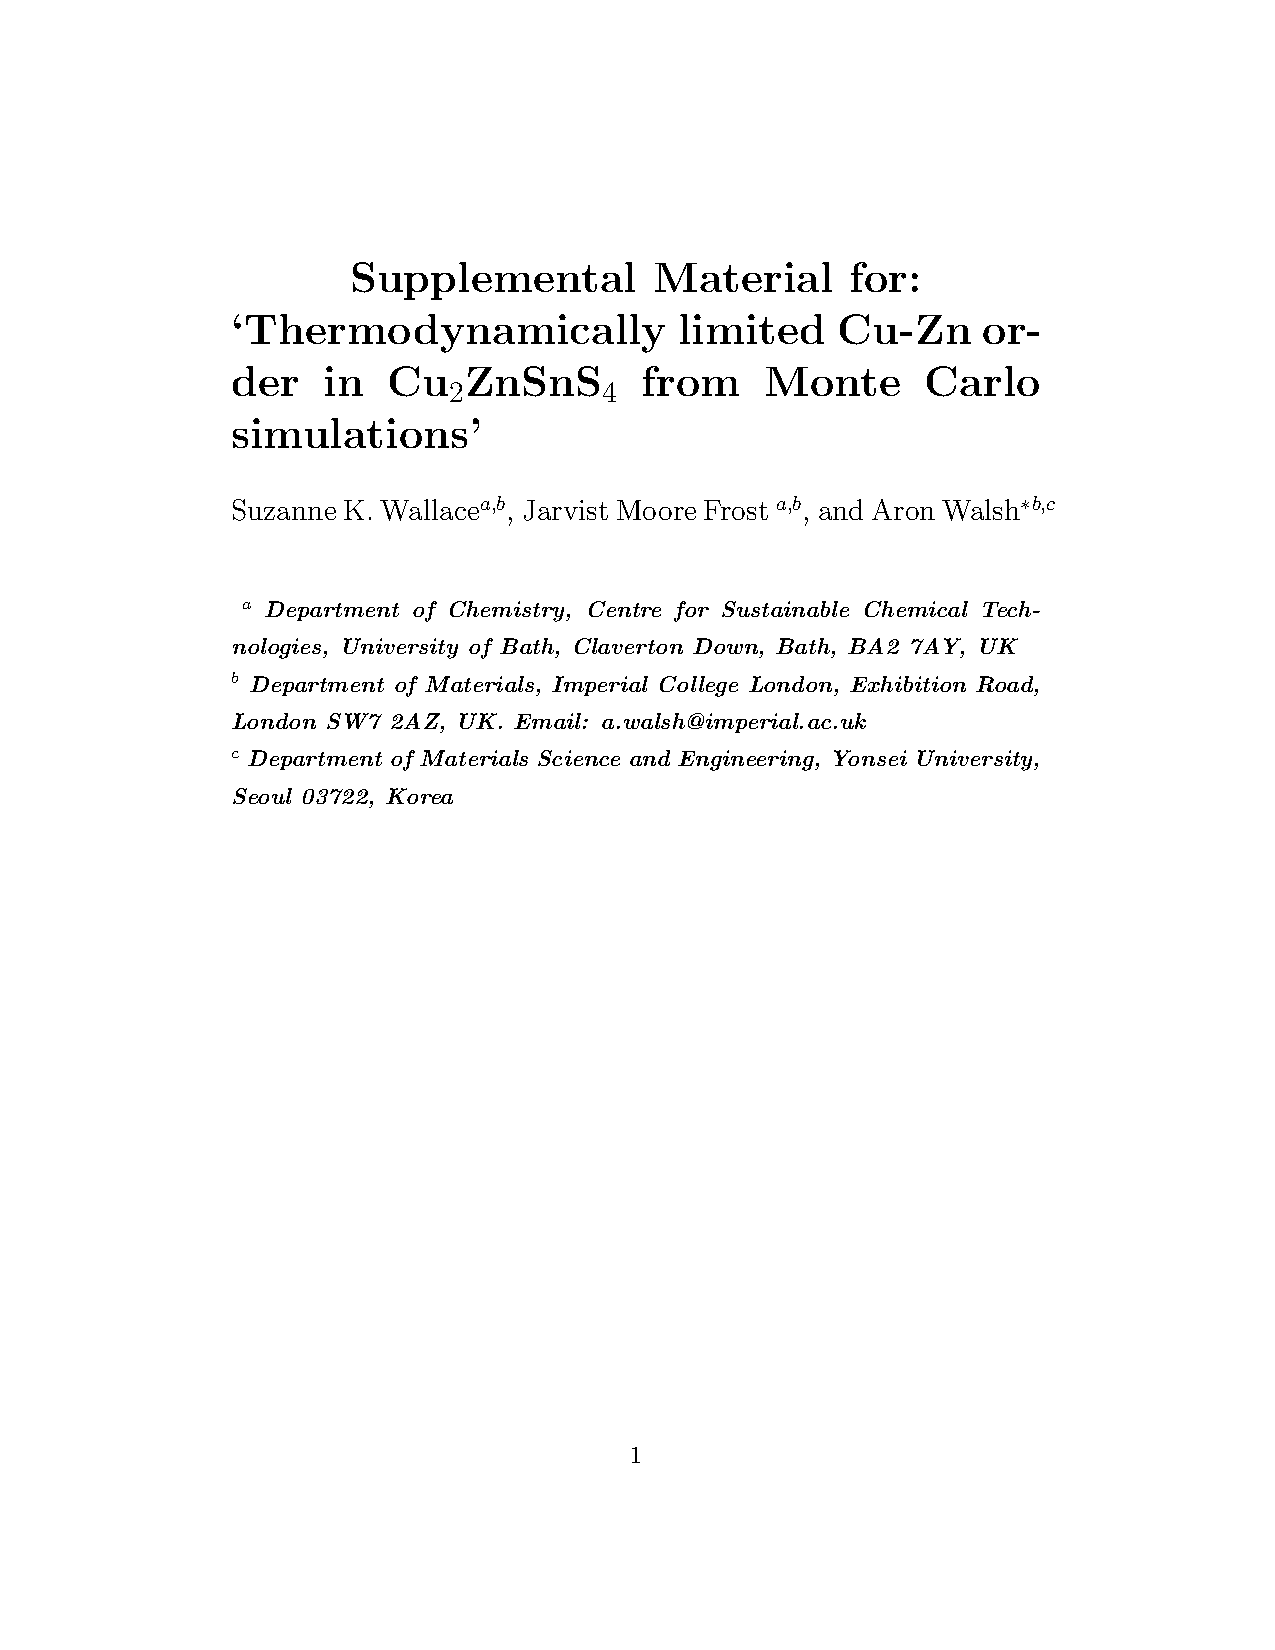
\includepdf[pages={1-},scale=1.0]{papers/Eris1_SI.pdf}


%\section{Outlook: Band tailing and modified defect physics from Cu-Zn disorder}
%\section{Outlook: Impact of Cu-Zn disorder on solar cell performance}\label{eris_future_work}
\section{Electronic band tailing in {\CZTS} from Cu-Zn disorder}

** Band tailing letter here **\\

Although $Cu_{Zn}^{-}$ and $Zn_{Cu}^{+}$ antisite defects have been predicted to produce only shallow defect levels within the band gap of the material \cite{defects_Chen}, their presence could be linked to band tailing in the material, as described in section \ref{defects_impact}. 
Point defects in an otherwise perfect lattice can be regarded as missing lattice atoms, which are replaced by lattice defects. Therefore for every defect that creates one or more levels in the band gap of the material, the same number of levels that would have been created by the atoms in the host lattice are missing. Additionally, the lattice atoms surrounding the defect relax into shifted positions and also create states that could be shifted slightly into the band gap \cite{thin_film_Boer}. All of these states contribute to perturbations in the band edge, such as that shown in Fig. \ref{pankove_elec_fluc}. Such a tail of band states into the band gap is often referred to as a Lifshitz tail \cite{Lifshitz1964}, it can be observed experimentally and is most noticeable in heavily doped and amorphous semiconductors \cite{thin_film_Boer}. 
\begin{figure}[h!]
  \centering
    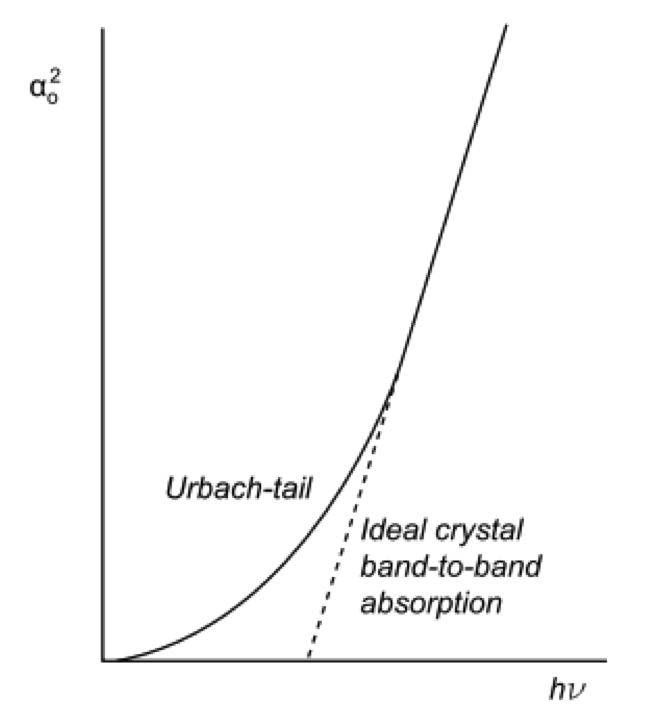
\includegraphics[width=0.45\textwidth]{figures/urbach_fig.png}
    \caption{Optical absorption spectrum of a typical direct band gap semiconductor with the absorption coefficient, $\alpha_{0}$, proportional to the extended density of states in the Urbach tail. Figure taken from reference \citenum{thin_film_Boer}.}
  \label{urbach_fig}
\end{figure}
For disorder due to defects with a correlation length on the order of interatomic spacing, the absorption coefficient, $\alpha_{0}$ (which was discussed as a key property for PV materials in section \ref{PV_properties}) shows a exponential decline. This effect, illustrated in figure \ref{urbach_fig}, is referred to as the Urbach tail \cite{Urbach1953} and is widely observed in disordered semiconductors \cite{thin_film_Boer}. Such tailing can be quantified by the Urbach energy, and it has recently been proposed that there is a direct link between the Urbach energy and open circuit voltage deficit in standard photovoltaic materials \cite{culprit, UrbachE_Voc}.

** Maybe move some content from theory impact of defects section here? **

As discussed in section \ref{CZTS_beyond_dilute}, concentrations of $[Cu_{Zn}^{-} + Zn_{Cu}^{+}]$ antisites in {\CZTS} are expected to be beyond the dilute limit. In this section therefore we calculate on-site electrostatic potentials of disordered configurations from our Monte Carlo simulations of on-lattice extended Cu-Zn disorder. Our model can be used to determine the contribution to band tailing just from fluctuations in the spatial distribution of electrostatic potential from the presence of charged $Cu_{Zn}^{-}$ and $Zn_{Cu}^{+}$ antisite defects. (**Note that our model can't account for any strain effects on band gap because it is fixed on lattice, but expect small contribution to band tailing from this effect due to similar ionic radii of Cu+ and Zn2+)

... Outline ideology for band tailing extension (s.d. or range of dist. of Cu and Sn potentials wrt T? and c.f. Q to infer band tailing of VBM and CBM with T respectively + inc. CZTS band structure from a paper, see eris lab book slides), quantify band tailing from this and also show 2D visuals of fluctuations using 2D histogram plots of Cu and Sn vs. mean of dist.?\\

+ See band tailing write up plan + this paper: https://www.sciencedirect.com/science/article/pii/S0927024817306062?via%3Dihub
\\

Possible extension to adapt MC model to explore possibility of disorder suppression in off-stoichiometric CZTS?\\

Plan for discussion of eris band tailing results:
\begin{itemize}
\item s.d. of potential distribution w.r.t T (smoothed over multiple random seed re-runs) - comparison between this and Q vs. T plot indicates difference between a macroscopic average and the microscopic fluctuations that will interact with photocarriers
\item Use range as indicator of band tailing (as opposed to s.d.)?
\item Histograms/ kde plots of potential distribution (normal dist or double pot?)
\item 2D on-site potential - mean potential histograms (comparisons for different random seeds, 72x72x72 and a hero 144x144x72)
\item Generate 1D plot along y=x to show two well and peak for 72x72x72 system... relate to band fluctuation schematics in literature?
\item Discuss if it is possible to infer that Sn-on-Zn antisites (which has been linked to defect clusters that impact band gap) may be more likely to form due to potential distribution. e.g. Sn4+ more likely to be on a Zn2+ site in negative potential region? c.f. end of S4 in doi: 10.1016/j.solmat.2017.11.005
\item Also note from (doi: 10.1016/j.solmat.2017.11.005) - 'clusters of Zn-Cu+ antisites have been observed by scanning transmission electron microscopy [40]'
\item Note use dielectric const for perfect CZTS (9.9) calculated by Sunghyun when converting units to V for potential because we are now interesting in potential in our perfect system (rather than scaling order-disorder transition T to exptl system with more physics than in present in our model)
\end{itemize}

%Look for Jarv's work on band tailing in MAPI to discuss how Eris could be similarly applied to extract band tails in CZTS\\

%Discuss NREL works on extended antisites? (see other notes on Sn disorder) Key paper for discussing Sn disorder: https://doi.org/10.1016/j.solmat.2017.11.005\\


\chapter{Screening for candidate photoferroic solar absorbers}\label{chap:screening}
\section{Candidate photoferroic minerals and predicted optoelectronic properties}

%Introductory paragraph + sulfosalts paper1 + include paper SI? (put in appendix?) \\

In the previous chapter, it was demonstrated that high concentrations of Cu-Zn disorder is inevitable in the solar absorber material {\CZTS} and the contribution of electrostatic potential fluctuations from this type of disorder to the observed band tailing was quantified. In this chapter, a screening procedure is conducted to look for alternative absorber materials. The motivation of this study was to identify candidate `photoferroic’ or photoactive ferroelectric materials. Photoferroic phenomena were outlined in section \ref{photoferroic}. The mechanisms behind such phenomena are not yet fully understood, however it may be possible to achieve improvements in solar cell performance from enhanced local carrier separation from the internal electric fields of polar crystals, possibly providing new pathways to achieving high-performance devices.
Additionally, the band tailing from prevalent cation disorder (as investigated for {\CZTS}) would be expected to be less prevalent in these materials (as has been demonstrated in AZTS **REF FROM PAPER* and BCTS **REF FROM PAPER**) due to the materials containing less chemically similar components.

This work was primarily conducted during a collaboration visit to Duke University with developers of the FHI-aims \cite{FHI-aims} electronic structure software package and calculations of spontaneous lattice polarisation were performed by Katrine Svane at the University of Bath.


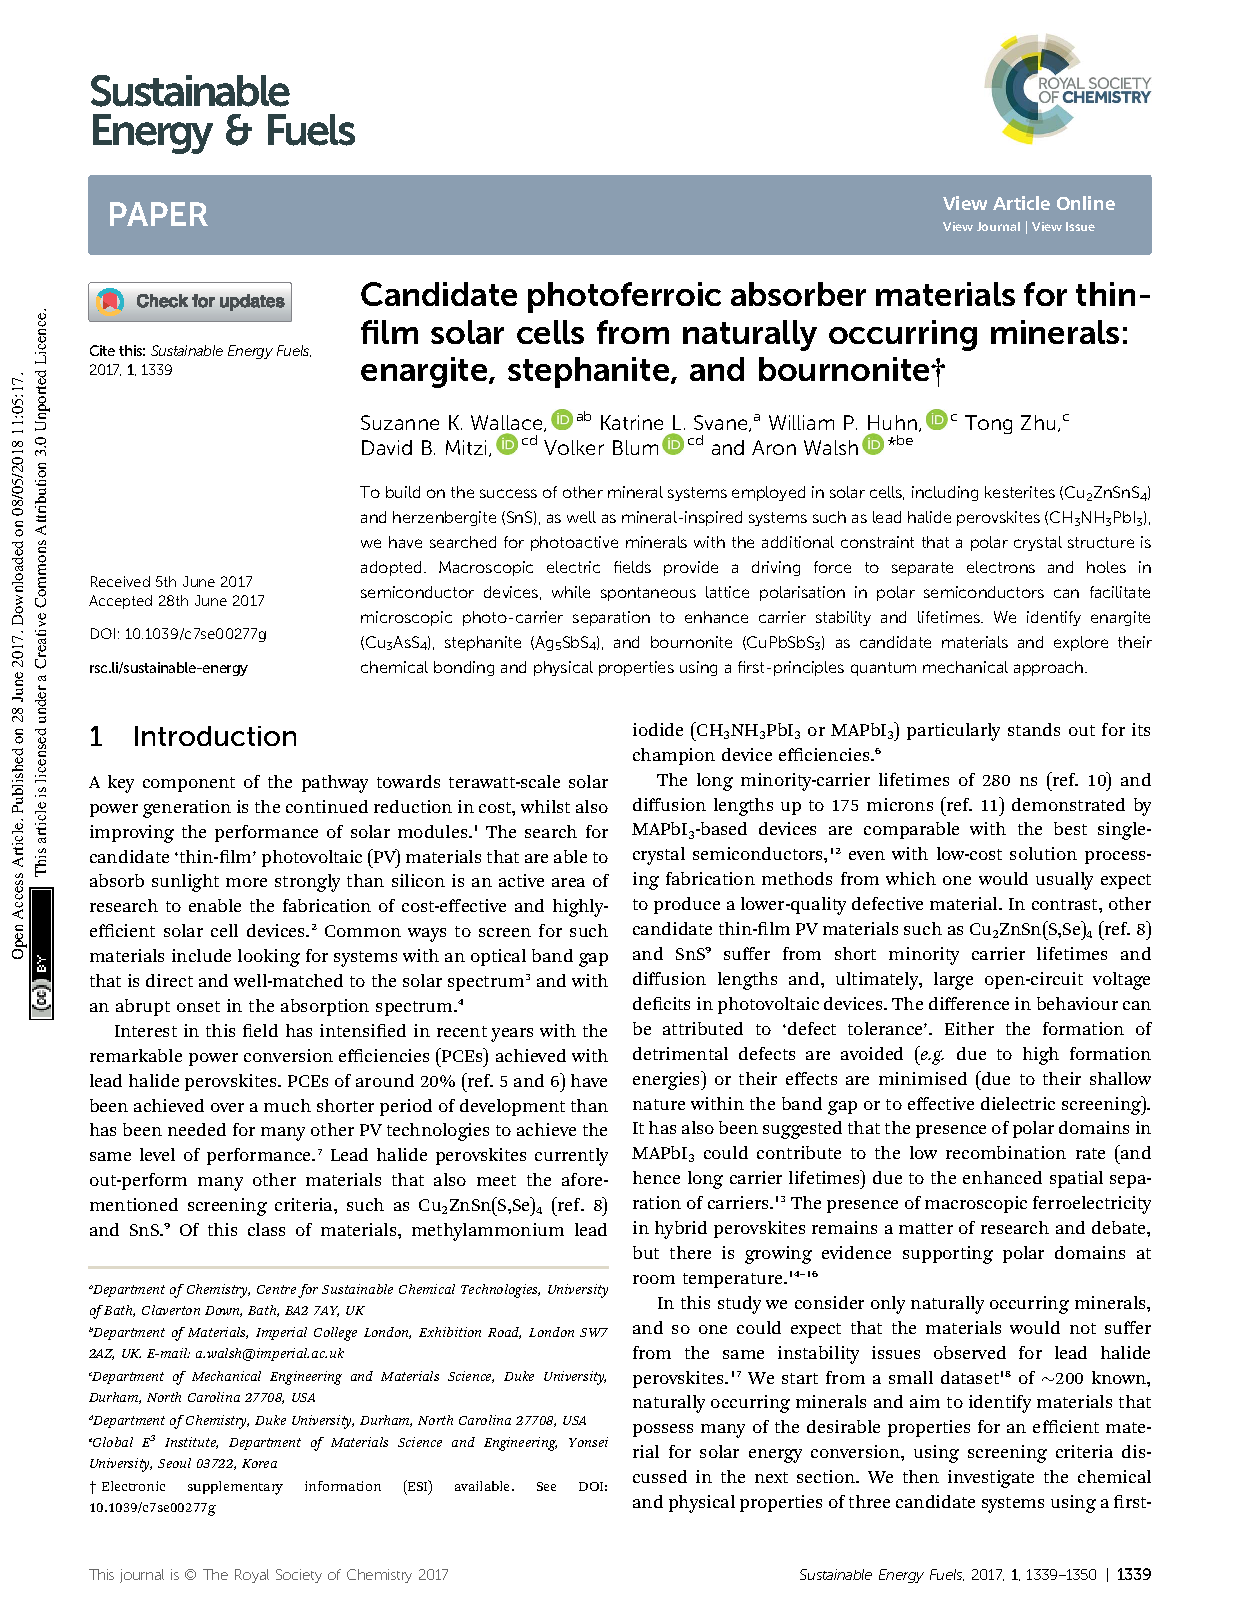
\includepdf[pages={1-},scale=1.0]{papers/sulfosalts1.pdf}
\includepdf[pages={1-},scale=1.0]{papers/sulfosalts1_SI.pdf}


\section{Outlook: Large-scale screening with material properties databases}

Overview of screening process:
\begin{itemize}
\item Stable - energy below convex hull
\item Less than or equal to 4 elements
\item Materials with toxic or rare elements ruled out?
\item Polar space group
\item Band gap 0 to 1.5 (N.B. materials project GGA roughly underestimates by 20%) – double check with Lee + citation???
\item Effective mass calculated with Boltztrapp (need to justify choice of T and carrier conc? Take optimal value for carrier conc on the assumption this could be tuned experimentally? And T as typical operating T of a solar cell? – double check exact values with Lee
\item Check slack channel for how we were screening effective mass tensor (first for average below threshold then discounted anything with one component above threshold to avoid materials with very anisotropic transport properties??
\end{itemize}


In the study in the previous section, three candidate photoferroic materials were identified from the dataset of approximately 200 naturally occurring minerals. This choice of initial dataset was motivated by the high stability that could be expected for naturally occurring minerals. However, with the availability of materials properties databases and tools for screening such databases, there are much larger search spaces for materials discovery and it may be possible to identify better materials from such a resource. For this reason, an ongoing study is being conducted in collaboration with Lee A. Burton to perform a similar screening procedure using the Materials Project \cite{materials_project}. Here, just the motivations, modified screening criteria and some preliminary results of this subsequent search are outlined.

As we do not start from a dataset of naturally occurring minerals in this extension, we limit our search space to only stable materials by considering only compounds with energies below the convex hull **GET MP REF FOR CONVEX HULL**. We also only consider compounds composed of 4 or less elements to avoid materials that are likely to be particularly challenging to synthesise. In the interests of identifying suitable candidates for large-scale and environmentally friendly solar cells, we rule out compounds containing rare or toxic elements **double check with Lee** (maybe just screened by abundance??).

After this initial screening, we apply similar screening criteria to the previous project. We also screen by polar space group but as opposed to using the streak colour as an indication that the band gap is likely to be within the visible range, we use the calculated band gaps for the compounds contained in the Materials Project database. Calculations for the material properties contained in the Materials Project database are performed at the GGA \cite{GGA}.
The underestimation of the band gaps in the Materials Project database is roughly 20% **GET REF**. We use 0 to 1.5 eV as the range of band gap for our candidates. Effective masses were calculated for the three candidate photoferroic minerals in the previous study, in this study high-throughput calculations of effective mass tensors are performed for ??? candidates using calculated band structure from the Materials Project and the BoltzTrapp code \cite{BoltzTrapp} with temperature set to the typical operating temperature of a solar cell at ?? and carrier concentration assumed to be ??. 
With this substantially larger number of candidate photoferroic materials, we were able to be more stringent in our standards for charge carrier effective masses. We first screened by the isotropic average… and then by components of the effective mass tensor so that we were left with candidates with the potential for with isotropically high carrier mobility.

Preliminary results: maybe just comment on number of candidates with m* for BOTH electrons and holes below 0.5 me? (Check with Lee) - 'This is an on-going work but so far results from the initial screening have shown ?? number of compounds that have polar space groups, band gaps within the range for solar absorption and effective masses for both electrons and holes less than 0.5m$_e$. Further work will involve a closer examination of their optoelectronic properties and potential as solar cell absorber layers.'\\

**Write intro, motivations for FE-PV and methods in the form of a paper intro for Lee?? – take some motivations from paper1 and refer to Kirchartz review + see other FE-PV lit on desktop **


\chapter{Theoretical insights for new solar absorbers}\label{chap:insights}
State that although we expect cation disorder to be less prevalent than Cu-Zn disorder in {\CZTS}, this does not rule out other limitations on performance (such as defects and non-optimal device architectures). Here we take inspiration from more mature or successful PV tech and use insights from theory to assess the potential of two of the three minerals from \autoref{chap:screening}.\\

Statement to justify choice of continuing study just for enargite and bournonite (high content of Ag in stephanite, solar cells already attempted with enargite, other interests in bournonite, etc (see start of sulfosalts defects write up)

\section{Band alignment for solar cell heterojunctions}\label{sulfosalt_band_alignment}
Introductory paragraph (new PV tech must be optimised layer-by-layer), barrier to utilisation of new tech, aim to use theory to accelerate process, often architectures optimised for different, more mature tech is used for new PV absorbers - not necessarily optimal! (e.g. of enargite paper and various others from band alignments paper intro) + sulfosalts band alignments paper\\

Although it may be possible to achieve photovoltaic energy conversion without a solar cell junction as described in section \ref{photoferroics}, a solar cell junction is likely to still be beneficial to provide a global driving force for carrier separation with internal electric fields allowing for improved local carrier separation and possible new pathways to achieving high-performance devices.\\

+ Add statement on personal contribution (Slabs cut by Yoyo, MD and ELS codes by Keith, calculations performed by me, ELS extended by me to include workflow for CBOs and VBOs of interest for PV)

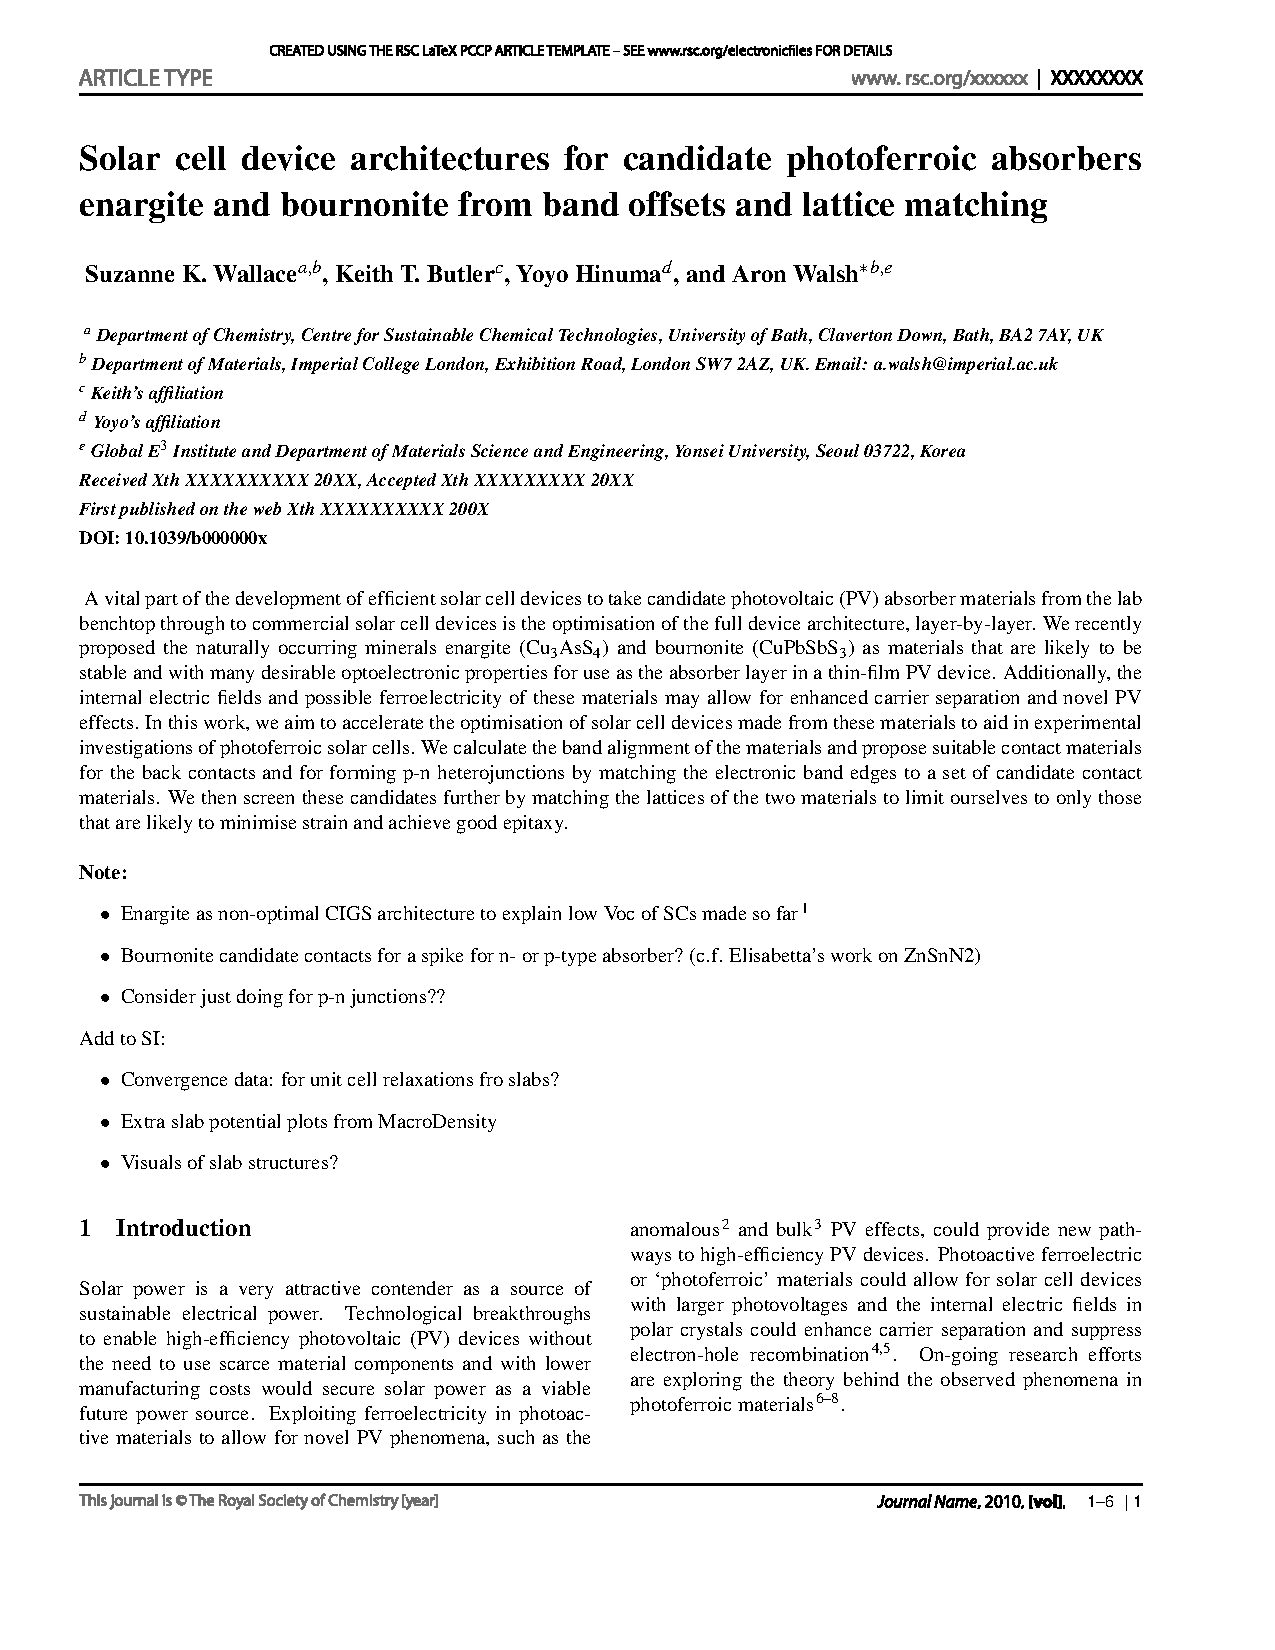
\includepdf[pages={1-},scale=1.0]{papers/sulfosalts_band_alignment_draft.pdf}

\section{Benchmarking point defect formation energies}\label{defect_benchmark}

Or rename benchmarking potential alignment for defect formation energies?? (If this work is using FNV in coFFEE, validate against VASP and quantumESPRESSO and then compare to GaAs cluster? (When introducing, refer back to methods section outlining finite-size correction, highlight need for reliable defect formation energies, read Thomas Durrant's paper that looks into different contributions to and check there for ref for inconsistent defect E's in the literature?)\\

Post-processing tools for the implementation of finite-size correction schemes to defect formation energies were integrated with the electronic structure code FHI-aims \cite{FHI-aims} for the study presented in section \ref{sulfosalt_defects}. This therefore provided an opportunity to benchmark defect formation energies calculated by different electronic structure codes with different post-processing finite-size correction schemes applied…

Nod to delta project DFT benchmark for bulk \cite{delta_project_paper} and highlight importance of a similar benchmark for defect calculations/ finite-size corrections to defect supercells.

Introduce paper for FHI-aims defects benchmark study with Volker and Tong + add statement on personal contribution?\\

Possibly different treatment for `jellium' than VASP and hence different correction? no pa??\\

Note from Komsa paper: Possibly contributions to need for pa from variations in the average value of the local pseudopotential which depends on the number and kind of atoms in the supercell, would not also be present in FHI-aims?


\section{Predicting and tuning defect-tolerance from electronic structure}\label{sulfosalt_defects}
State that we expect extended cation disorder to be present to a lesser extent than in CZTS due to less chemical similarity? Also that understanding defect physics from a point-defect perspective is an important foundation to build for understanding the complicate defect physics of a multi-component material? e.g. next step would be pairs, etc.

Introductory paragraph (power of predicting this property - determine materials worthy of further study, inform synthesis procedures for faster optimisation) + sulfosalts defects work as complete as possible (write last, aim to have as much of paper written as possible first!)\\

+ Add statement on personal contribution

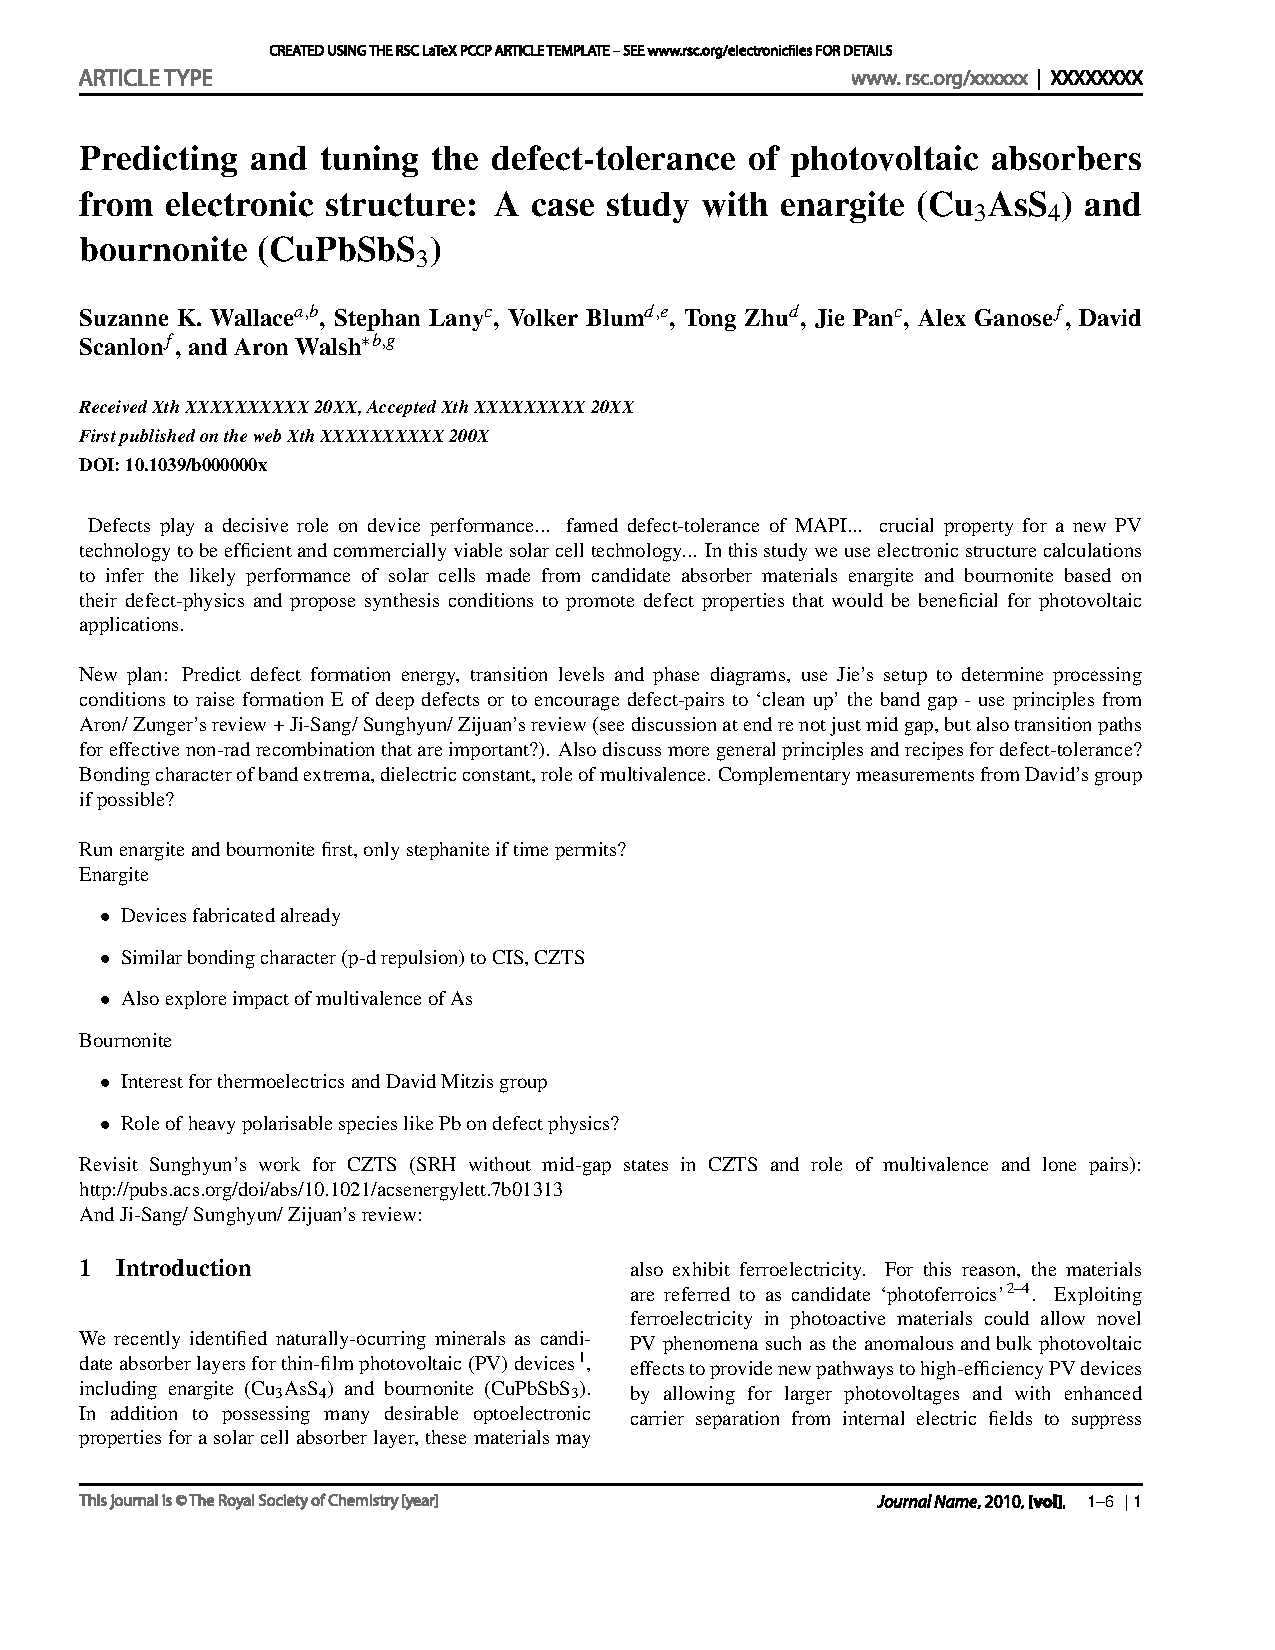
\includepdf[pages={1-},scale=1.0]{papers/sulfosalts_defects_draft.pdf}

%\section{The quest for universal descriptors for predicting solar cell performance}
%Mention high-throughput material screening (in broader research field) here again.\\

%See Thomas Kirchartz recent review 'What makes a good solar cell'.\\

%Nod to SQ, SLME and Thomas Kirchartz's detailed balance theoretical maximum efficiencies when introducing this section? + works on predicting defect-tolerance by MIT\\ 


%Dielectric function review? (finished/ collab with Jacob or as finished as far as possible?) Comment on dielectric constants of enargite and bournonite calculated as part of defects study here?\\




\chapter{Closing remarks}

Taken from old thesis plan:
\begin{itemize}
\item Extensions with Eris for CZTS cation disorder and band tailing (further investigate origin and suppression of band tailing)
\item Off-stoichiometric types (explanation for higher-performance of Cu-poor?) and Sn disorder
\item Maybe broader implications from Eris – defect formation energy in a typical supercell method perhaps not applicable in materials with high levels of disorder? (If Sn point defect formation E can be reduced by presence of Cu-Zn disorder)
\item Insights (and limitations) of PV performance predictions for sulfosalts
\item New pathways to high-performance… or added complexity in fabrication? Depolarisation fields at device interfaces? Static FE domains like internal diodes? (c.f. mobile FE proposed in MAPI due to mobile MA+)
\item Extra considerations for tuning electric fields in photoferroic devices, especially at interfaces and modelling carrier transport?
\item We hope that the predictions made for sulfosalts will aid in experimental investigation of photoferroic solar cells
\item Many pathways for further investigations of the sulfosalts (materials are a playground for a materials scientist!)
\item Many on-going works to better understand FE-PV phenomena to open up possibility of exploiting the phenomena in devices? (refer to works of Rappe and at NREL?)
\item Possibility of studying effect of Rashba splitting on PL lifetimes with bournonite by tuning splitting with applied E-field? (provide insights onto role this feature of band structure of MAPI is having on performance?)
\end{itemize}

\section{Cu-Zn disorder in {\CZTS} solar cells}
Summarise results of paper1 + could also adapt our MC model to simulate off-stoichiometric CZTS to see if Cu-Zn disorder could be suppressed in these systems. Summarise results of band tailing letter. If band tails from Cu-Zn disorder are small, maybe here would be a good point to mention possibility of reduced Sn defect formation energy in regions of inhomogeneous electrostatic potential due to Cu-Zn disorder??

\section{Candidate photoferroic absorbers in solar cells}
Overview of optical properties predicted in paper1. Opportunity to explore possible FE-PV phenomena in these materials. Suggested device architecture and processing conditions for minimising Voc loss at junctions and deep level defects + overview of expected defect properties of the materials.

\appendix
% appendices come here

%\chapter{Appendix}
%\section{Review of photoluminescence spectra of \CZTS}\label{CZTS_PL_section}
%Photoluminescence (PL) spectroscopy is a popular method to inspect solar cell materials as it does not require a full functioning device and can be a powerful tool for probing defects in semiconductors. There are a large number of possible optical transitions that can be detected by PL measurements, some of which were illustrated in figure \ref{PL_transitions}. For this reason, low-temperature PL can be a particularly powerful tool for probing defects as energy level occupancy is dependent upon temperature and so not all PL recombinations will occur at the same temperature, allowing for the isolation of different types of recombination transitions \cite{spatial_resolved_book}. There are also other variations in the set up of a PL measurement that can be altered to provide more information on the band structure and how it is altered by the presence of defects. Firstly the intensity of the laser can be increased to determine if states are localized (such as those introduced by defects) or extended states (such as the conduction and valence bands) by if it is possible to saturate the states in the case of localized states such that an increase in laser intensity no longer increases the intensity of the PL peak \cite{Gershon}. Secondly, time-resolved PL (TRPL) measurements  can be used to differentiate between recombination mechanisms with different carrier lifetimes. Slower optical transitions usually involve carriers in localized states, whereas faster transitions usually involve delocalized states \cite{Gershon}.

%Several PL studies have been performed on kesterite-structured samples of {\CZTS}, Cu$_2$ZnSnSe$_4$ and alloys of the two. PL measurements have been performed on both full devices and polycrystalline thin-films \cite{band_tail, Gershon, Gershon_ref18, Romero, Miyamoto, Unold} and single crystals \cite{Halliday, Levcenko, Hones}. In addition studies such as reference \citenum{Halliday} compare the PL spectra for varying compositions of the sample, whereas in reference \citenum{band_tail} measurements on both CIGSSe and CZTSSe thin films are performed in an attempt to account for the difference in the performance of these two technologies by comparing their defect-influenced PL emission spectra. Polycrystalline samples are more similar to those likely to be used in thin-film CZTS photovoltaic devices, however comparison between those measurements with single crystal measurements could enable the isolation of recombination at grain boundaries from those due to bulk defects. Also measurements performed on single crystals as close to perfectly stoichiometric {\CZTS} as possible are likely to be the most directly relatable to our simulations on bulk systems. However one feature common to all of the PL spectra from studies on kesterite samples is clear evidence of defects and disorder from the observed band tailing. The PL spectra of kesterite samples usually features a much broader peak than that observed in CIGSSe samples, such as that shown in figure \ref{CZTS+CIGS_PL}. The energy of the maximum PL peaks of kesterite samples is also usually considerably red-shifted compared to the energy of the band gap. These two features are usually attributed to band tailing caused by either spatial band gap variations or electrostatic potential fluctuations in the absorber material, which were discussed in section \ref{PL_section}.  Both effects lead to a non-zero density of states (DOS) within the band gap \cite{culprit, band_tail}. 
%Measurements performed in reference \citenum{band_tail} found the tailing in CZTSSe to be roughly twice as severe as that observed in higher-performing CIGSSe devices.

%\cite{band_tail} = Mitzi PL paper, \cite{Gershon} = first paper in overview, \cite{Gershon_ref18} = previous work with good overview of PL

%However, there is some disagreement in the literature about the main recombination mechanisms that could explain the observed PL spectra. Of the measurements performed on single crystals, reference \citenum{Levcenko} perform measurements on near-stoichiometric CZTS crystals and report a free-to-bound transition between the conduction band and an acceptor level. In reference \citenum{Hones}, donor-acceptor-pair (DAP) transitions are reported for large single grains of CZTS, whereas in reference \citenum{Halliday} where measurements are performed on CZTS single-crystals of varying composition, they report PL measurements through spatially fluctuating band states as would be expected from either spatial band gap variations or electrostatic potential fluctuations from heavy defect compensation. Therefore in bulk monograins of CZTS PL band-to-impurity, DAP and spatially fluctuating band-type recombinations have all been reported and the exact sources, or rather associated defects, for these recombination mechanisms are not yet known \cite{Gershon_ref18}.

%For measurements performed on polycrystalline kesterite samples, some studies attribute the spectra to spatially fluctuating band tail states \cite{Romero}, whereas others suggest that recombination in CZTS is dominated by the distinct energy levels introduced by DAPs \cite{Unold, Miyamoto}. In other studies, an explanation that is almost a combination of the two is proposed \cite{Gershon, Gershon_ref18}. These studies refer to a quasi-donor-acceptor-pair (QDAP) model, where the word `quasi' is used to indicate a deviation from the classical DAP model for recombinations, such as that shown in figure \ref{PL_transitions}, due to interactions between defects. In reference \citenum{Gershon_ref18} they note that distinguishing between DAP recombination and spatially fluctuating band tails caused by spatially varying densities of ionized donor and acceptor defects is particularly complicated as a high density of compensating DAPs is necessarily co-incident with spatial fluctuation in electrostatic potential. In the same work, they note that the dominance of donor and acceptor pairs on PL spectra is in agreement with theoretical predictions such as those by Chen et al \cite{defect1} that antisite DAPs such as $[Cu_{Zn}^{-} + Zn_{Cu}^{+}]$ should be abundant due to the low formation energy of the defect complex and also experimental observations of cation disorder by neutron diffraction, synchrotron radiation x-ray diffraction and aberration corrected scanning transmission electron microscopy respectively \cite{Schorr, CZTS_Xray, CZTS_TEM}.


\addcontentsline{toc}{chapter}{Bibliography}
\bibliographystyle{unsrt}
\bibliography{thesis.bib}

\end{document}